
%% bare_jrnl_compsoc.tex
%% V1.4b
%% 2015/08/26
%% by Michael Shell
%% See:
%% http://www.michaelshell.org/
%% for current contact information.
%%
%% This is a skeleton file demonstrating the use of IEEEtran.cls
%% (requires IEEEtran.cls version 1.8b or later) with an IEEE
%% Computer Society journal paper.
%%
%% Support sites:
%% http://www.michaelshell.org/tex/ieeetran/
%% http://www.ctan.org/pkg/ieeetran
%% and
%% http://www.ieee.org/

%%*************************************************************************
%% Legal Notice:
%% This code is offered as-is without any warranty either expressed or
%% implied; without even the implied warranty of MERCHANTABILITY or
%% FITNESS FOR A PARTICULAR PURPOSE! 
%% User assumes all risk.
%% In no event shall the IEEE or any contributor to this code be liable for
%% any damages or losses, including, but not limited to, incidental,
%% consequential, or any other damages, resulting from the use or misuse
%% of any information contained here.
%%
%% All comments are the opinions of their respective authors and are not
%% necessarily endorsed by the IEEE.
%%
%% This work is distributed under the LaTeX Project Public License (LPPL)
%% ( http://www.latex-project.org/ ) version 1.3, and may be freely used,
%% distributed and modified. A copy of the LPPL, version 1.3, is included
%% in the base LaTeX documentation of all distributions of LaTeX released
%% 2003/12/01 or later.
%% Retain all contribution notices and credits.
%% ** Modified files should be clearly indicated as such, including  **
%% ** renaming them and changing author support contact information. **
%%*************************************************************************


% *** Authors should verify (and, if needed, correct) their LaTeX system  ***
% *** with the testflow diagnostic prior to trusting their LaTeX platform ***
% *** with production work. The IEEE's font choices and paper sizes can   ***
% *** trigger bugs that do not appear when using other class files.       ***                          ***
% The testflow support page is at:
% http://www.michaelshell.org/tex/testflow/


\documentclass[10pt,journal,compsoc]{IEEEtran}
% \documentclass[10pt,compsoc,cspaper]{IEEEtran}
% \documentclass[10pt,peerreviewca,compsoc]{IEEEtran}
%.cls has not been installed into the LaTeX system files,
% manually specify the path to it like:
% \documentclass[10pt,journal,compsoc]{../sty/IEEEtran}





% Some very useful LaTeX packages include:
% (uncomment the ones you want to load)


% *** MISC UTILITY PACKAGES ***
%
%\usepackage{ifpdf}
% Heiko Oberdiek's ifpdf.sty is very useful if you need conditional
% compilation based on whether the output is pdf or dvi.
% usage:
% \ifpdf
%   % pdf code
% \else
%   % dvi code
% \fi
% The latest version of ifpdf.sty can be obtained from:
% http://www.ctan.org/pkg/ifpdf
% Also, note that IEEEtran.cls V1.7 and later provides a builtin
% \ifCLASSINFOpdf conditional that works the same way.
% When switching from latex to pdflatex and vice-versa, the compiler may
% have to be run twice to clear warning/error messages.






% *** CITATION PACKAGES ***
%
\ifCLASSOPTIONcompsoc
  % IEEE Computer Society needs nocompress option
  % requires cite.sty v4.0 or later (November 2003)
  \usepackage[nocompress]{cite}
\else
  % normal IEEE
  \usepackage{cite}
\fi
% cite.sty was written by Donald Arseneau
% V1.6 and later of IEEEtran pre-defines the format of the cite.sty package
% \cite{} output to follow that of the IEEE. Loading the cite package will
% result in citation numbers being automatically sorted and properly
% "compressed/ranged". e.g., [1], [9], [2], [7], [5], [6] without using
% cite.sty will become [1], [2], [5]--[7], [9] using cite.sty. cite.sty's
% \cite will automatically add leading space, if needed. Use cite.sty's
% noadjust option (cite.sty V3.8 and later) if you want to turn this off
% such as if a citation ever needs to be enclosed in parenthesis.
% cite.sty is already installed on most LaTeX systems. Be sure and use
% version 5.0 (2009-03-20) and later if using hyperref.sty.
% The latest version can be obtained at:
% http://www.ctan.org/pkg/cite
% The documentation is contained in the cite.sty file itself.
%
% Note that some packages require special options to format as the Computer
% Society requires. In particular, Computer Society  papers do not use
% compressed citation ranges as is done in typical IEEE papers
% (e.g., [1]-[4]). Instead, they list every citation separately in order
% (e.g., [1], [2], [3], [4]). To get the latter we need to load the cite
% package with the nocompress option which is supported by cite.sty v4.0
% and later. Note also the use of a CLASSOPTION conditional provided by
% IEEEtran.cls V1.7 and later.





% *** GRAPHICS RELATED PACKAGES ***
%
\ifCLASSINFOpdf
   \usepackage[pdftex]{graphicx}
%   declare the path(s) where your graphic files are
   \graphicspath{{../pdf/}{../jpeg/}}
%   and their extensions so you won't have to specify these with
%   every instance of \includegraphics
   \DeclareGraphicsExtensions{.pdf,.jpeg,.png}
\else
  % or other class option (dvipsone, dvipdf, if not using dvips). graphicx
  % will default to the driver specified in the system graphics.cfg if no
  % driver is specified.
   \usepackage[dvips]{graphicx}
%   declare the path(s) where your graphic files are
   \graphicspath{{../eps/}}
%   and their extensions so you won't have to specify these with
%   every instance of \includegraphics
   \DeclareGraphicsExtensions{.eps}
\fi
% graphicx was written by David Carlisle and Sebastian Rahtz. It is
% required if you want graphics, photos, etc. graphicx.sty is already
% installed on most LaTeX systems. The latest version and documentation
% can be obtained at: 
% http://www.ctan.org/pkg/graphicx
% Another good source of documentation is "Using Imported Graphics in
% LaTeX2e" by Keith Reckdahl which can be found at:
% http://www.ctan.org/pkg/epslatex
%
% latex, and pdflatex in dvi mode, support graphics in encapsulated
% postscript (.eps) format. pdflatex in pdf mode supports graphics
% in .pdf, .jpeg, .png and .mps (metapost) formats. Users should ensure
% that all non-photo figures use a vector format (.eps, .pdf, .mps) and
% not a bitmapped formats (.jpeg, .png). The IEEE frowns on bitmapped formats
% which can result in "jaggedy"/blurry rendering of lines and letters as
% well as large increases in file sizes.
%
% You can find documentation about the pdfTeX application at:
% http://www.tug.org/applications/pdftex






% *** MATH PACKAGES ***
%
\usepackage{amsmath}
% A popular package from the American Mathematical Society that provides
% many useful and powerful commands for dealing with mathematics.
%
% Note that the amsmath package sets \interdisplaylinepenalty to 10000
% thus preventing page breaks from occurring within multiline equations. Use:
%\interdisplaylinepenalty=2500
% after loading amsmath to restore such page breaks as IEEEtran.cls normally
% does. amsmath.sty is already installed on most LaTeX systems. The latest
% version and documentation can be obtained at:
% http://www.ctan.org/pkg/amsmath





% *** SPECIALIZED LIST PACKAGES ***
%
%\usepackage{algorithmic}
% algorithmic.sty was written by Peter Williams and Rogerio Brito.
% This package provides an algorithmic environment fo describing algorithms.
% You can use the algorithmic environment in-text or within a figure
% environment to provide for a floating algorithm. Do NOT use the algorithm
% floating environment provided by algorithm.sty (by the same authors) or
% algorithm2e.sty (by Christophe Fiorio) as the IEEE does not use dedicated
% algorithm float types and packages that provide these will not provide
% correct IEEE style captions. The latest version and documentation of
% algorithmic.sty can be obtained at:
% http://www.ctan.org/pkg/algorithms
% Also of interest may be the (relatively newer and more customizable)
% algorithmicx.sty package by Szasz Janos:
% http://www.ctan.org/pkg/algorithmicx




% *** ALIGNMENT PACKAGES ***
%
%\usepackage{array}
% Frank Mittelbach's and David Carlisle's array.sty patches and improves
% the standard LaTeX2e array and tabular environments to provide better
% appearance and additional user controls. As the default LaTeX2e table
% generation code is lacking to the point of almost being broken with
% respect to the quality of the end results, all users are strongly
% advised to use an enhanced (at the very least that provided by array.sty)
% set of table tools. array.sty is already installed on most systems. The
% latest version and documentation can be obtained at:
% http://www.ctan.org/pkg/array


% IEEEtran contains the IEEEeqnarray family of commands that can be used to
% generate multiline equations as well as matrices, tables, etc., of high
% quality.




% *** SUBFIGURE PACKAGES ***
%\ifCLASSOPTIONcompsoc
%  \usepackage[caption=false,font=footnotesize,labelfont=sf,textfont=sf]{subfig}
%\else
%  \usepackage[caption=false,font=footnotesize]{subfig}
%\fi
% subfig.sty, written by Steven Douglas Cochran, is the modern replacement
% for subfigure.sty, the latter of which is no longer maintained and is
% incompatible with some LaTeX packages including fixltx2e. However,
% subfig.sty requires and automatically loads Axel Sommerfeldt's caption.sty
% which will override IEEEtran.cls' handling of captions and this will result
% in non-IEEE style figure/table captions. To prevent this problem, be sure
% and invoke subfig.sty's "caption=false" package option (available since
% subfig.sty version 1.3, 2005/06/28) as this is will preserve IEEEtran.cls
% handling of captions.
% Note that the Computer Society format requires a sans serif font rather
% than the serif font used in traditional IEEE formatting and thus the need
% to invoke different subfig.sty package options depending on whether
% compsoc mode has been enabled.
%
% The latest version and documentation of subfig.sty can be obtained at:
% http://www.ctan.org/pkg/subfig




% *** FLOAT PACKAGES ***
%
%\usepackage{fixltx2e}
% fixltx2e, the successor to the earlier fix2col.sty, was written by
% Frank Mittelbach and David Carlisle. This package corrects a few problems
% in the LaTeX2e kernel, the most notable of which is that in current
% LaTeX2e releases, the ordering of single and double column floats is not
% guaranteed to be preserved. Thus, an unpatched LaTeX2e can allow a
% single column figure to be placed prior to an earlier double column
% figure.
% Be aware that LaTeX2e kernels dated 2015 and later have fixltx2e.sty's
% corrections already built into the system in which case a warning will
% be issued if an attempt is made to load fixltx2e.sty as it is no longer
% needed.
% The latest version and documentation can be found at:
% http://www.ctan.org/pkg/fixltx2e


%\usepackage{stfloats}
% stfloats.sty was written by Sigitas Tolusis. This package gives LaTeX2e
% the ability to do double column floats at the bottom of the page as well
% as the top. (e.g., "\begin{figure*}[!b]" is not normally possible in
% LaTeX2e). It also provides a command:
%\fnbelowfloat
% to enable the placement of footnotes below bottom floats (the standard
% LaTeX2e kernel puts them above bottom floats). This is an invasive package
% which rewrites many portions of the LaTeX2e float routines. It may not work
% with other packages that modify the LaTeX2e float routines. The latest
% version and documentation can be obtained at:
% http://www.ctan.org/pkg/stfloats
% Do not use the stfloats baselinefloat ability as the IEEE does not allow
% \baselineskip to stretch. Authors submitting work to the IEEE should note
% that the IEEE rarely uses double column equations and that authors should try
% to avoid such use. Do not be tempted to use the cuted.sty or midfloat.sty
% packages (also by Sigitas Tolusis) as the IEEE does not format its papers in
% such ways.
% Do not attempt to use stfloats with fixltx2e as they are incompatible.
% Instead, use Morten Hogholm'a dblfloatfix which combines the features
% of both fixltx2e and stfloats:
%
% \usepackage{dblfloatfix}
% The latest version can be found at:
% http://www.ctan.org/pkg/dblfloatfix




%\ifCLASSOPTIONcaptionsoff
%  \usepackage[nomarkers]{endfloat}
% \let\MYoriglatexcaption\caption
% \renewcommand{\caption}[2][\relax]{\MYoriglatexcaption[#2]{#2}}
%\fi
% endfloat.sty was written by James Darrell McCauley, Jeff Goldberg and 
% Axel Sommerfeldt. This package may be useful when used in conjunction with 
% IEEEtran.cls'  captionsoff option. Some IEEE journals/societies require that
% submissions have lists of figures/tables at the end of the paper and that
% figures/tables without any captions are placed on a page by themselves at
% the end of the document. If needed, the draftcls IEEEtran class option or
% \CLASSINPUTbaselinestretch interface can be used to increase the line
% spacing as well. Be sure and use the nomarkers option of endfloat to
% prevent endfloat from "marking" where the figures would have been placed
% in the text. The two hack lines of code above are a slight modification of
% that suggested by in the endfloat docs (section 8.4.1) to ensure that
% the full captions always appear in the list of figures/tables - even if
% the user used the short optional argument of \caption[]{}.
% IEEE papers do not typically make use of \caption[]'s optional argument,
% so this should not be an issue. A similar trick can be used to disable
% captions of packages such as subfig.sty that lack options to turn off
% the subcaptions:
% For subfig.sty:
% \let\MYorigsubfloat\subfloat
% \renewcommand{\subfloat}[2][\relax]{\MYorigsubfloat[]{#2}}
% However, the above trick will not work if both optional arguments of
% the \subfloat command are used. Furthermore, there needs to be a
% description of each subfigure *somewhere* and endfloat does not add
% subfigure captions to its list of figures. Thus, the best approach is to
% avoid the use of subfigure captions (many IEEE journals avoid them anyway)
% and instead reference/explain all the subfigures within the main caption.
% The latest version of endfloat.sty and its documentation can obtained at:
% http://www.ctan.org/pkg/endfloat
%
% The IEEEtran \ifCLASSOPTIONcaptionsoff conditional can also be used
% later in the document, say, to conditionally put the References on a 
% page by themselves.




% *** PDF, URL AND HYPERLINK PACKAGES ***
%
%\usepackage{url}
% url.sty was written by Donald Arseneau. It provides better support for
% handling and breaking URLs. url.sty is already installed on most LaTeX
% systems. The latest version and documentation can be obtained at:
% http://www.ctan.org/pkg/url
% Basically, \url{my_url_here}.


% \usepackage{algorithm, algpseudocode}
\usepackage{mathptmx}
\usepackage{tabu} 
\usepackage{booktabs}
\usepackage{here}
\usepackage{xcolor}
\usepackage{url}
% \usepackage{enumerate}
\usepackage{enumitem}


% *** Do not adjust lengths that control margins, column widths, etc. ***
% *** Do not use packages that alter fonts (such as pslatex).         ***
% There should be no need to do such things with IEEEtran.cls V1.6 and later.
% (Unless specifically asked to do so by the journal or conference you plan
% to submit to, of course. )


% correct bad hyphenation here
\hyphenation{op-tical net-works semi-conduc-tor}


\begin{document}
%
% paper title
% Titles are generally capitalized except for words such as a, an, and, as,
% at, but, by, for, in, nor, of, on, or, the, to and up, which are usually
% not capitalized unless they are the first or last word of the title.
% Linebreaks \\ can be used within to get better formatting as desired.
% Do not put math or special symbols in the title.
\title{TimeTubesX: A Query-Driven Visual Exploration of Observable, Photometric, and Polarimetric Behaviors of Blazars}
%
%
% author names and IEEE memberships
% note positions of commas and nonbreaking spaces ( ~ ) LaTeX will not break
% a structure at a ~ so this keeps an author's name from being broken across
% two lines.
% use \thanks{} to gain access to the first footnote area
% a separate \thanks must be used for each paragraph as LaTeX2e's \thanks
% was not built to handle multiple paragraphs
%
%
%\IEEEcompsocitemizethanks is a special \thanks that produces the bulleted
% lists the Computer Society journals use for "first footnote" author
% affiliations. Use \IEEEcompsocthanksitem which works much like \item
% for each affiliation group. When not in compsoc mode,
% \IEEEcompsocitemizethanks becomes like \thanks and
% \IEEEcompsocthanksitem becomes a line break with idention. This
% facilitates dual compilation, although admittedly the differences in the
% desired content of \author between the different types of papers makes a
% one-size-fits-all approach a daunting prospect. For instance, compsoc 
% journal papers have the author affiliations above the "Manuscript
% received ..."  text while in non-compsoc journals this is reversed. Sigh.
\author{Naoko Sawada,~\IEEEmembership{Student Member,~IEEE,}
        Makoto Uemura,~%\IEEEmembership{}
        Johanna Beyer,~\\%\IEEEmembership{Member,~IEEE}
        Hanspeter Pfister,~\IEEEmembership{Senior Member,~IEEE,}
        and~Issei~Fujishiro,~\IEEEmembership{Member,~IEEE}% <-this % stops a space
\IEEEcompsocitemizethanks{\IEEEcompsocthanksitem N. Sawada is with Keio University.\protect\\
% M. Shell was with the Department
% of Electrical and Computer Engineering, Georgia Institute of Technology, Atlanta,
% GA, 30332.\protect\\
% note need leading \protect in front of \\ to get a newline within \thanks as
% \\ is fragile and will error, could use \hfil\break instead.
E-mail: naoko.sawada@fj.ics.keio.ac.jp.
\IEEEcompsocthanksitem M. Uemura is with Hiroshima University.\protect\\
E-mail: uemuram@hiroshima-u.ac.jp.
\IEEEcompsocthanksitem J. Beyer and H. Pfister are with Harvard University.\protect\\
E-mail: \{jbeyer, pfister\}@seas.harvard.edu.
\IEEEcompsocthanksitem I. Fujishiro is with Keio University and Hangzhou Dianzi University.\protect\\
E-mail: fuji@ics.keio.ac.jp.}% <-this % stops an unwanted space
\thanks{Manuscript received May 9, 2020: revised August 26, 2020.}}
% \author{Michael~Shell,~\IEEEmembership{Member,~IEEE,}
%         John~Doe,~\IEEEmembership{Fellow,~OSA,}
%         and~Jane~Doe,~\IEEEmembership{Life~Fellow,~IEEE}% <-this % stops a space
% \IEEEcompsocitemizethanks{\IEEEcompsocthanksitem M. Shell was with the Department
% of Electrical and Computer Engineering, Georgia Institute of Technology, Atlanta,
% GA, 30332.\protect\\
% % note need leading \protect in front of \\ to get a newline within \thanks as
% % \\ is fragile and will error, could use \hfil\break instead.
% E-mail: see http://www.michaelshell.org/contact.html
% \IEEEcompsocthanksitem J. Doe and J. Doe are with Anonymous University.}% <-this % stops an unwanted space
% \thanks{Manuscript received April 19, 2005; revised August 26, 2015.}}

% note the % following the last \IEEEmembership and also \thanks - 
% these prevent an unwanted space from occurring between the last author name
% and the end of the author line. i.e., if you had this:
% 
% \author{....lastname \thanks{...} \thanks{...} }
%                     ^------------^------------^----Do not want these spaces!
%
% a space would be appended to the last name and could cause every name on that
% line to be shifted left slightly. This is one of those "LaTeX things". For
% instance, "\textbf{A} \textbf{B}" will typeset as "A B" not "AB". To get
% "AB" then you have to do: "\textbf{A}\textbf{B}"
% \thanks is no different in this regard, so shield the last } of each \thanks
% that ends a line with a % and do not let a space in before the next \thanks.
% Spaces after \IEEEmembership other than the last one are OK (and needed) as
% you are supposed to have spaces between the names. For what it is worth,
% this is a minor point as most people would not even notice if the said evil
% space somehow managed to creep in.



% The paper headers
\markboth{Journal of \LaTeX\ Class Files,~Vol.~14, No.~8, August~2020}%
{Sawada \MakeLowercase{\textit{et al.}}: TimeTubesX: A Query-Driven Visual Exploration of Observable, Photometric, and Polarimetric Behaviors of Blazars}
% The only time the second header will appear is for the odd numbered pages
% after the title page when using the twoside option.
% 
% *** Note that you probably will NOT want to include the author's ***
% *** name in the headers of peer review papers.                   ***
% You can use \ifCLASSOPTIONpeerreview for conditional compilation here if
% you desire.



% The publisher's ID mark at the bottom of the page is less important with
% Computer Society journal papers as those publications place the marks
% outside of the main text columns and, therefore, unlike regular IEEE
% journals, the available text space is not reduced by their presence.
% If you want to put a publisher's ID mark on the page you can do it like
% this:
%\IEEEpubid{0000--0000/00\$00.00~\copyright~2015 IEEE}
% or like this to get the Computer Society new two part style.
%\IEEEpubid{\makebox[\columnwidth]{\hfill 0000--0000/00/\$00.00~\copyright~2015 IEEE}%
%\hspace{\columnsep}\makebox[\columnwidth]{Published by the IEEE Computer Society\hfill}}
% Remember, if you use this you must call \IEEEpubidadjcol in the second
% column for its text to clear the IEEEpubid mark (Computer Society jorunal
% papers don't need this extra clearance.)



% use for special paper notices
%\IEEEspecialpapernotice{(Invited Paper)}



% for Computer Society papers, we must declare the abstract and index terms
% PRIOR to the title within the \IEEEtitleabstractindextext IEEEtran
% command as these need to go into the title area created by \maketitle.
% As a general rule, do not put math, special symbols or citations
% in the abstract or keywords.
% \IEEEtitleabstractindextext{%
% \begin{abstract}
% The abstract goes here.
% \end{abstract}

% % Note that keywords are not normally used for peerreview papers.
% \begin{IEEEkeywords}
% Computer Society, IEEE, IEEEtran, journal, \LaTeX, paper, template.
% \end{IEEEkeywords}}
\IEEEtitleabstractindextext{%
\begin{abstract}
Blazars are celestial bodies of high interest to astronomers. 
In particular, through the analysis of photometric and polarimetric observations of blazars, 
astronomers aim to understand the physics of the blazar’s relativistic jet. 
However, it is challenging to recognize correlations and time variations of the observed polarization, intensity, and color of the emitted light. In our prior study, we proposed TimeTubes to visualize a blazar dataset as a 3D volumetric tube. In this paper, we build primarily on the TimeTubes representation of blazar datasets to present a new visual analytics environment named TimeTubesX, 
into which we have integrated sophisticated feature and pattern detection techniques for effective location of observable and recurring time variation patterns in long-term, multi-dimensional datasets. 
Automatic feature extraction detects time intervals corresponding to well-known blazar behaviors. 
Dynamic visual querying allows users to search long-term observations for time intervals similar to a time interval of interest (query-by-example) or a sketch of temporal patterns (query-by-sketch). 
Users are also allowed to build up another visual query guided by the time interval of interest found in the previous process and refine the results. We demonstrate how TimeTubesX has been used successfully by domain experts for the detailed analysis of blazar datasets and report on the results.

% Blazars are celestial bodies of high interest to astronomers. In particular, astronomers aim to understand, through analysis of photometric and polarimetric observations of blazars, the physics of the blazar's relativistic jet. However, it is challenging to recognize time variation of and correlations among the observed polarization, intensity, and color of the emitted light. 
% We proposed TimeTubes, through which a blazar dataset is visualized as a 3D volumetric tube. In this paper, we develop TimeTubesX, a new visual analytics environment for blazar datasets that extends our previous TimeTubes. 
% In this paper, we describe TimeTubesX, a new visual analytics environment for blazar datasets that extends our previous TimeTubes, through which a blazar dataset is visualized as a 3D volumetric tube.
% We have integrated sophisticated feature and pattern detection techniques into TimeTubesX that allow for effective location of observable and recurring time variation patterns in long-term, multi-dimensional datasets. 
% Blazars are celestial bodies of high interest to astronomers. In particular, astronomers aim to understand, through analysis of photometric and polarimetric observations,
% the physics of the relativistic jet that is ejected from a blazar's center.
% However, it is challenging to recognize time variation patterns of and correlations among the observed polarization, intensity, and color of the emitted light. 
% We have previously proposed TimeTubes, through which a blazar dataset is visualized as a 3D volumetric tube.
% In this paper, we develop TimeTubesX, a new visual analytics environment for blazar observations that extends our previous TimeTubes.
% We have integrated sophisticated feature and pattern detection techniques into TimeTubesX that allow for the effective location of observable and recurring time variation patterns in long-term, multi-dimensional datasets.
% Automatic feature extraction methods detect time intervals that include well-known blazar behaviors. 
% Dynamic visual querying methods allow users to search long-term observations for time intervals similar to a time interval of interest (query-by-example) or a sketch of time variation patterns (query-by-sketch). 
% The result of a query can be directly re-used as an input for another dynamic visual query.
% This iterative pattern search allows users to build up another query guided by the interesting time interval found in the previous process and to refine results. 
% We demonstrate how TimeTubesX has been successfully used by domain experts for the detailed analysis of blazar observations and report on the results.
\end{abstract}

% Note that keywords are not normally used for peerreview papers.
\begin{IEEEkeywords}
Visual analytics, feature extraction, visual query, multi-dimensional, time-dependent visualization, astrophysics, blazar
\end{IEEEkeywords}}

% make the title area
\maketitle


% To allow for easy dual compilation without having to reenter the
% abstract/keywords data, the \IEEEtitleabstractindextext text will
% not be used in maketitle, but will appear (i.e., to be "transported")
% here as \IEEEdisplaynontitleabstractindextext when the compsoc 
% or transmag modes are not selected <OR> if conference mode is selected 
% - because all conference papers position the abstract like regular
% papers do.
\IEEEdisplaynontitleabstractindextext
% \IEEEdisplaynontitleabstractindextext has no effect when using
% compsoc or transmag under a non-conference mode.



% For peer review papers, you can put extra information on the cover
% page as needed:
% \ifCLASSOPTIONpeerreview
% \begin{center} \bfseries EDICS Category: 3-BBND \end{center}
% \fi
%
% For peerreview papers, this IEEEtran command inserts a page break and
% creates the second title. It will be ignored for other modes.
\IEEEpeerreviewmaketitle


\ifCLASSOPTIONcompsoc
\IEEEraisesectionheading{\section{Introduction}\label{sec:introduction}}
\else
\section{Introduction}
\label{sec:introduction}
\fi
% Blazar are an important topic of researches in astronomy and high-energy astrophysics. 
\IEEEPARstart{B}{lazars} are important to the studies of astronomy and high-energy astrophysics. 
They are in a class of extremely bright galactic nuclei called active galactic nuclei (AGN) that shoot out a stream of particles from their center~\cite{Antonucci1993a}. 
A relativistic jet is angled directly toward the Earth from a central black hole of a blazar (see Fig.~\ref{fig:blazar}).
However, relatively little is known about the intricate physics of these jets' structures. %about these structures.
% To demystify the intricate physics of the jet's structures,
Astronomers pay careful attention to blazars
because the jet radiation of blazars is more amplified than that of other AGN.
% Astronomers pay careful attentions to blazars
%Blazars are a class of extremely bright galactic nuclei with a supermassive black hole at their center~\cite{Antonucci1993a}. 
%They emit a relativistic jet directly angled toward the Earth, 
%as illustrated in \autoref{fig:blazar}.
%The astronomers pay careful attentions to blazars 
%because the physics of the jet is mysterious even nowadays.
% To predict the effects of the magnetic field on the jet,
To demystify the jets' structures,
astronomers need to analyze correlations and time variations in photometric and polarimetric observations of the emitted light.
% of observed polarization, intensity, and color of the emitted light.
% However, it is challenging for them to manually identify recurring patterns or similar time intervals from long-term, multi-dimensional observations.
%for effectively understanding dynamic variations in and feature causality among multiple variables.
%Our previous application provides visual data fusion for datasets from multiple observatories and diverse interactions
%to accomplish more effective data analysis~\cite{Fujishiro2018}.
%To identify known blazar behaviors or recurring patterns, astronomers need to meticulously analyze their high-dimensional data.
For instance, a light burst (i.e., \textit{flare}) is one of the most distinctive behaviors of blazars~\cite{Bednarek1999, Atoyan2001}.
Identifying flares requires astronomers to scrutinize correlations of the emitted light's intensity with polarization and/or color, because looking at the time variation of the intensity alone is insufficient. %always varies finely.
%
In addition to flares, some astronomers are interested in the polarization direction of light and whether it rotates~\cite{Marscher2008, Uemura2017}.
%In addition to flares, some astronomers reported that the polarization direction of the light sometimes rotates~\cite{Marscher2008, Uemura2017}.
It is a controversial question in astronomy whether such \textit{rotations} are real or due to random variations of polarization.
To verify polarization rotations, correlations of the polarization with the intensity and/or the color are crucial.
% Moreover, astronomers would like to locate time intervals with common features in time variations.
Moreover, astronomers would like to locate time intervals with common features in  time variations
to understand what happens inside the jet.
However, it is an overwhelming process for them to manually examine all time intervals in long-term, multi-dimensional datasets in order to detect these significant patterns and validate hypotheses.
%those including flares/rotations and validating a specific hypothesis.

To support these exploration challenges, 
we have developed \textit{TimeTubesX}, a new visual analytics environment for blazar observations. 
%
This novel system extends our previous visualization scheme, called \textit{TimeTubes}~\cite{Fujishiro2018}, 
which allows users to interactively explore multi-dimensional, time-dependent observation datasets of blazars in a unique 3D tube view and to combine datasets from multiple observatories into a single visualization session termed \emph{visual data fusion}.
%, which focused on visualizing blazar observations in a unique 3D view.
%
%that integrates our previous TimeTubes view.
%Previously, we proposed \textit{TimeTubes}~\cite{Fujishiro2018}, a unique 3D visualization for blazar observations that allowed users to interactively explore their high-dimensional datasets more intuitively, and to combine datasets from multiple observatories into a single visualization session.
%on top of the previous TimeTubes.
In TimeTubesX, we place more focus on visual analysis and automated and semi-automated approaches for feature and pattern detection.
%We have developed advanced feature extraction mechanisms for TimeTubesX, consisting of automatic and interactive approaches.
The automatic feature extraction methods, which are in part an extension of our previous work~\cite{Sawada2018}, detect time intervals corresponding to well-known blazar behaviors, such as flares and rotations.
%with reference to the astronomers' reports,
The dynamic visual querying methods, on the other hand, are useful for analysis and detection of recurring patterns that have not yet been explored in detail. 

% This paper extends our previous short paper about the automatic feature extraction for blazar observations~\cite{Sawada2018}, but we have significantly improved our detection algorithms. 
% The primary contributions of this paper are three-fold. 
Our first contribution is a detailed goal and task analysis performed with domain experts to design a visual analytics framework for blazar observations. 
Subsequently, we have designed and implemented TimeTubesX as a web-based and open-source system. 
Our second contribution lies in powerful automatic feature extraction methods for well-known blazar behaviors and an intuitive visual query platform for multi-dimensional, time-dependent data.
Finally, as our third contribution, we demonstrate the usefulness of TimeTubesX through experiments with a synthetic dataset, real data analyses, and feedback from domain experts.
We envision that our visual query mechanisms could be applied to multi-dimensional, time-series datasets in other domains to help users identify recurring patterns or similar time intervals.
% \begin{itemize}
%     \item %Implementation of a new web-based visual analysis environment,termed TimeTubesX, for blazar observations based on analysis ofspecific sets of domain goals and involved tasks.
%     A detailed goal and task analysis performed with our domain experts to design a visual analysis framework for blazar observations. 
%     Subsequently, we have designed and implemented TimeTubesX as a web-based and open-source system. 
%     \item Powerful automatic feature extraction methods for well-known blazar behaviors and an intuitive visual query platform for time-dependent, multi-dimensional data.
%     \item A demonstration of the usefulness of TimeTubesX based on a real data analysis by a domain expert.
% \end{itemize}
%We fully improved the detection algorithms.

% We first review related work
% in \autoref{sec:relatedWork}, before describing our target data and domain goals and tasks in \autoref{sec:domainAnalysis}.
% \autoref{sec:systemDesign} introduces the system design of TimeTubesX.
% \autoref{sec:automaticExtraction}, \autoref{sec:visualQuery}, and \autoref{sec:otherFunctions} present details on our feature and pattern detection methods.
% We demonstrate the effectiveness of the proposed intuitive feature extraction through an evaluation case in \autoref{sec:evaluation}.
% In \autoref{sec:discussion}, we discuss feedback from domain experts and limitations of TimeTubesX.
% We conclude this paper in \autoref{sec:conclusion}.



% For example, the black hole ejects a jet almost at the speed of light, 
% but what accelerates it is not clear yet.

% if they look over animated scatterplots, 
% which have been commonly used in the astrophysical community.

% Regarding the behaviors of blazars, there are a lot of mysterious parts. 
% When the relativistic jet in a blazar forms a burst, the light from a blazar gets highly luminous, that is called a flare. 
% Flare is one of the most characteristic behaviors. 
% Some astronomers report that the polarization direction of the light from blazars sometimes rotates. 
% However, it is controversial in astronomy whether the rotations are real ones or fake ones caused by random variations of polarization.
% To verify polarization rotations, astronomers need to scrutinize correlations among other observation variables. 
% On the other hand, there can exist undiscovered phenomena of blazars. 
% It is significant to explore recurring patterns of time variations or correlations among variables. 
% Nevertheless, deliberate analysis across multiple variables is indispensable.
% To address these difficulties, we introduce a novel feature extraction for blazar observations.
% It supports two types of feature extraction: Automatic extraction and visual query. 
% The automatic extraction can squeeze only observable time intervals from (multiple) long-term observations, 
% whereas the visual query can find time intervals similar to a region of interest (ROI) or shape of interest (POI). 

% When the relativistic jet in a blazar forms a burst, the light from a blazar gets highly luminous, that is called a flare. 

% In other words, there are too many peaks of the intensity to identify notable flares 
% without regard for correlations between the intensity and other parameters.

% It takes time to visit all time intervals to find flares or rotations and inspect correlations among the other parameters.

% this paper presents a feature extraction for blazar observations as an advanced function of TimeTubes, 
% which offers the astronomers time intervals including known blazar phenomena, such as flares and rotations, 
% and those similar to a region or shape of interest.
% The feature extraction provides two approaches: automatic and interactive.

%about visualization techniques for astronomical data and feature extraction techniques 
\section{Related work\label{sec:relatedWork}}
Our target blazar datasets are multi-dimensional (mD), semi-structured, and time-dependent.
This section reviews prior work in astronomical visualization and visual query systems for mD and time-series data. 


\subsection{Visualization for Astronomical Data}\label{sec:relatedAstronomy}
Most astronomers work on analyzing signals from distant celestial bodies, as measured from the Earth~\cite{Kent2017}. 
%Astronomers make much account of observing and analyzing signals from distant celestial bodies
%because they cannot travel just to see the bodies with their naked eyes~\cite{Kent2017}.
% Li et al.~\cite{Li2007} visualize positional and data-inherent uncertainties of large-scale 3D astronomical simulations.
% For multi-wavelength astronomical data, Li and Hanson~\cite{Li2008} propose a system for visual analysis across multiple datasets.
% %Li and Hanson~\cite{Li2008} tackle 3D visualization for multi-wavelength astronomical data from multiple data sources, which realizes easy visual analysis across multiple datasets.
% Baines et al.~\cite{Baines2017} develop a web-based data discovery portal, ESASky, for exploring multi-wavelength sky data.
% GalStamps~\cite{McCurdy2019} is a visual analytics tool for both real and simulated galaxy observations,
% which realizes analysis across multiple different visualization, such as scatterplots and parallel coordinate plots.
% Though many techniques have been developed for astronomical data, there are no other effective techniques for blazar observations, except for our early attempt~\cite{Fujishiro2018}.
ESASky~\cite{Baines2017} and OpenSpace~\cite{Bock2020} provide views for parts of the sky that are integrated from multiple data sources.
Almryde et al.~\cite{Almryde2016} visualize dark matter halos’ temporal evolution of position, mass, and radial velocity. 
% Various types of telescopes are used to observe the sky or particular celestial bodies in different wavelengths 
% because visible light observation does not provide enough data to appreciate the nature of the universe.
% observing only visible light is not enough to appreciate the real nature of the universe.
Li et al.~\cite{Li2008} realize easy visual analysis across multi-wavelength datasets.
IGM-Vis~\cite{Burchett2019} is a visual analytics tool for quasar sightline data.
% propose 3D view for galaxies and quasar sightlines and 2D views for spectrum for the analysis of intergalactic medium and circumgalactic medium.
Some approaches~\cite{Haroz2008, Li2008, Preston2016, McCurdy2019, Burchett2019} provide linked-view visualization systems that allow users to explore multiple types of visualizations for deeper analyses.
Many techniques have been developed for analysis of astronomical data, 
but typically, blazar researchers have been using animated scatterplots (see Section~\ref{sec:VisualEncoding}) 
because there were no other effective techniques for blazar observations prior to our early attempt, TimeTubes~\cite{Fujishiro2018}.
For more efficient data analysis with TimeTubesX, we introduce feature and pattern detection methods for blazar datasets, a part of which is an extension of our previous paper~\cite{Sawada2018}.

\subsection{Visual Queries}\label{sec:relatedFeature}
Visual query systems allow users to intuitively search for patterns of interest in their data.
%The two most common options are \emph{query-by-example} and \emph{query-by-sketch}.
%Query-by-example and query-by-sketch interfaces are powerful approaches to querying data intuitively. 
Query-by-example aims to find data samples that are similar to a user-specified example,
% However, they do not address how to find the initial interesting data samples. 
whereas query-by-sketch allows users to directly draw the shape of interest.
% , yet the techniques have to deal with the user-introduced uncertainties of sketches.

\textsf{Query-by-example.\ }
% QBE for univariate data
%In these systems, users select an example from their data, that serves as the query for the rest of the dataset.% excerpt a part of time series for their query.
Hochheiser and Shneiderman~\cite{Hochheiser2004} propose TimeSearcher, a visual exploration tool for time-series data. Users can select portions of timelines by the use of rectangular widgets like Timeboxes~\cite{Buono2005} and Search Boxes~\cite{Buono2008}.
%where the users are allowed to select portions of timelines by putting boxes, termed Timeboxes~\cite{Buono2005} or Search Boxes~\cite{Buono2008}.
Holz and Feiner~\cite{Holz2009} propose a relaxed selection technique for time intervals, through which users define the level of similarity either by the input speed or by spatial deviation from an original timeline.
The idea of detecting the input speed inspired our sketching interface.
However, their interactions are geared only toward univariate time-series data and are not appropriate for our mD blazar data.
%
%to allow ones to select a time interval and to define the level of similarity simultaneously
%by detecting either sketching speed or spatial deviation from an original timeline.
%Their interactions work effectively only for univariate time-series data.

% QBE for multivariate data
Query-by-example methods for mD data have also been proposed.
Martin and Ward~\cite{Martin2005} describe brushing techniques for visualizations,
such as scatterplots matrices and parallel coordinate plots.
Elmqvist et al. propose interactions for constructing visual queries with star plots~\cite{Elmqvist2007} and multiple scatterplots~\cite{Elmqvist2008}.
Scribble query~\cite{Nielsen2016} introduces touch interaction for forming visual queries
through parallel coordinate plots by scribbling axes. 
Several works have focused on unstructured mD datasets~\cite{Martin2005,Elmqvist2007,Nielsen2016}, 
%The techniques in \cite{Martin2005}, \cite{Elmqvist2007}, and \cite{Nielsen2016} effectively work for unstructured mD datasets, 
but they are not versatile enough for understanding correlations among our idiosyncratic variables (see Section~\ref{sec:BlazarData}), and they do not support queries for structured time-series data.
The scatterplots by Martin and Ward~\cite{Martin2005} and Elmqvist et al.~\cite{Elmqvist2008} can be partially useful for structured data, but they cannot be applied to time-series data.

% QBS
\textsf{Query-by-sketch.\ } 
%Users may sketch the shape of interest for their query.
Early examples of sketch-based queries include QuerySketch~\cite{Wattenberg2001} for temporal databases and QueryLines~\cite{Ryall2005} for approximate queries. 
%QuerySketch~\cite{Wattenberg2001} is a sketch-based visual query tool for a temporal database.
%QueryLines~\cite{Ryall2005} allows the users to draw a query involving soft constraints and preferences.
TimeSketch~\cite{Eichmann2015} supports pen and touch-based query specification but focuses only on univariate time-series data.

% symbolic approximation
%Query-by-sketch interfaces have to handle ambiguities of hand-drawn sketches. 
To deal with the ambiguities of hand-drawn sketches, several systems discretize the input query and datasets into symbolic or quantized representations~\cite{Muthumanickam2016,ruta2019sax}.
%The input query and time series are discretized into symbolic representations to cope with uncertainties of a hand-drawn sketch in \cite{Muthumanickam2016} and \cite{ruta2019sax}.
%
Alternatively, Correll and Gleicher~\cite{Correll2016} define invariants for hand-drawn sketches. % to deal with uncertainties of sketches. 
Mannino and Abouzied~\cite{Mannino2018} provide a matching algorithm that takes human sketching errors into account.
The sketching interactions of Qetch~\cite{Mannino2018} inspired our query-by-sketch interface.
Both techniques target univariate time-series data.
%
Shao et al.~\cite{Shao2014} introduce sketch-based queries for large sets of scatterplots
in which the system supports users with shadow-drawing suggestions. %, which we use as an inspiration for our fact-driven querying\autoref{sec:factDrivenQuerying}.
The suggestions allow users to draw a pattern based on actual values, not on their imaginations.
We use this idea as an inspiration for our fact-guided querying (see Section~\ref{sec:factDrivenQuerying}).
%users are allowed to draw a pattern with the help of shadow-drawing suggestions,
%due to which the input sketch is not just a fiction by the users but based on fact.
%It influences the concept of our fact-driven querying, as discussed in \autoref{sec:factDrivenQuerying}.
While these systems support querying structured mD data, they cannot be applied to time-series data.

% QBS for volume data
Several sketch-based techniques for multi-scalar volume data allow users to select regions of a 3D object through an ordinary 2D painting tool.
The techniques by Owada et al.~\cite{Owada2005} and Igarashi et al.~\cite{Igarashi2016} extract a plausible 3D region from the volume
by following contours or isosurfaces, respectively.
Tzeng et al.~\cite{Tzeng2003} present a method for specifying high-dimensional classification functions for the volume
by brushing regions of interest and uninterest. % and those of uninterest.
BrainGazer~\cite{Bruckner2009} provides simple interactions for the selection of a region of interest in the volume
by drag-and-drop functionality.
% clicking on and dragging a 3D object. 
These techniques target only multi-scalar volume data. 

\textsf{Combination of query-by-example and query-by-sketch.\ }
Query-by-example techniques do not address how to find the initial interesting data samples, 
% users have to first identify an interesting data point in their dataset,
while query-by-sketch techniques must surmount the user-introduced uncertainties of sketches.
Combination of both styles helps to resolve the trade-off, as addressed by 
Bernard et al.~\cite{Bernard2010} and Lee et al.~\cite{Lee2019}. 
The system by Bernard et al.~\cite{Bernard2010} supports univariate time-series data, while the one by Lee et al.~\cite{Lee2019} supports unstructured time-series data.
% To get the best of both worlds, TimeTubesX supports automatic feature extraction as wells as query-by-example and query-by-sketch interactions.
To get the best of both worlds, TimeTubesX supports both querying interactions.
%
%To compensate these shortcomings, 
%we go together with both styles to build a new integrated feature extraction system 
%with both styles.

% because standard visualizations like scatterplots, star plots, parallel coordinate plots is not enough 
% for the astronomers to understand correlations among idiosyncratic variables (see Sec.~\ref{sec:BlazarData}) to build their query.


% % QBE for univariate data
% There are many query-by-example techniques which can deal with univariate datasets.
% Hochheiser and Shneiderman~\cite{Hochheiser2004} propose a visual exploration tool for time-series data, named TimeSearcher,
% where users are allowed to select portions of timeline by putting boxes, Timeboxes~\cite{Buono2005}.
% Search Box~\cite{Buono2008}, an augmented version of Timebox, allows users to change the shape of the selected pattern 
% and provides a series of characteristic patterns to prune timelines. 
% % SOMFlow~\cite{Sacha2018} is a visual analytic tool which can interactively refine clusters based on query-by-example using self-organizing maps.
% Holz and Feiner~\cite{Holz2009} propose a relaxed selection technique for time-series data.
% The technique allows users to select a time interval and define the level of similarity simultaneously
% by detecting either sketching speed or spatial deviation from an original timeline.
% These methods are effective only for univariate datasets, 
% so their interactions can not be directly applied to multivariate datasets.

% % QBE for multivariate data
% There also exist query-by-example methods for multivariate non-time-varying datasets.
% Martin and Ward~\cite{Martin2005} describe the design of brushing techniques for multi-dimensional data with various visualizations, 
% like scatterplot matrices, parallel coordinate plots, and the like.
% DataMeadow~\cite{Elmqvist2007} also provides interactions for constructing visual queries for multi-dimensional data 
% with star plots by adding filtering constraints to each axis of star plots. 
% Elmqvist et al.~\cite{Elmqvist2008} propose a new interface for interactively building queries for a multi-dimensional dataset 
% by providing smooth transition animation between scatterplots in a similar way to rolling a dice. 
% Scribble query, proposed by Nielsen et al.~\cite{Nielsen2016}, introduces a touch interaction 
% for visually forming queries for a multi-dimensional dataset
% through parallel coordinate plots by scribbling axes to select categories or ranges.
% They can deal with non-time-varying multivariate datasets, 
% but standard visualizations like scatterplots, star plots, parallel coordinate plots is not enough 
% for astronomers to understand correlations among idiosyncratic variables (see Sec.~\ref{sec:BlazarData}) to build their query.



% As detailed in Sec.~\ref{sec:BlazarData},
% in the target blazar datasets of TimeTubesX, 
% two structured polarization parameters describe linear polarization of the light
% and two retinal parameters explain the brightness and color.
% In other words, 

% Astrophysics can be said to be the ultimate remote sensing,

% Visualizations for simulated data have been extensively studied in astronomy.
% Haroz et al.~\cite{Haroz2008} visualize multiple simulation results,
% where they colorize particles to express uncertainties in time-varying cosmological particle data.
% Kahler et al.~\cite{Kahler2002a} render simulations of the evolution of the first star in the universe.
% The gas distribution is expressed by opacities, whereas temparature is by colors.
% Jensen et al.~\cite{Jensen2001} present a physical model of the night sky seen on the Earth.
% Genetti~\cite{Genetti2002} simulates and visualizes Orion Nebula from various viewpoints.
% Magnor et al.~\cite{Magnor2005} present an interactive visualization tool for realistically rendered dust distributions around illuminating stars.

% We present visualizations for observed or measured data in astronomy.
% McDonald and Montgomery~\cite{McDonald2012} visualize high-resolution laser altimeter data of the Moon.
% By utilizing a colormap optimized by a combination of hue and brightness,
% users are allowed to distinguish high and low altitude place.
% Additionally, the system enables users to measure the distance and slope of the lunar surface interactively.

% EASYSky visualizes multiple archives and allows users to visually identify the data source.
% OpenSpace~\cite{Bock2020} is an integrated environment for data from both observed and simulated data,
% to interactively explore the known universe.
% and supports research in astronomy and space science as well as science communication in educational situations.

% consisting of structured properties for the polarization of the light and retinal properties for the intensity and color.

% Feature extraction results in eliciting useful information from large or long-term data~\cite{Laxman2006}.
% Many methods for finding out patterns or outstanding time variations are proposed~\cite{WarrenLiao2005, Zhang2005, Rosner1983, Palshikar2009}.
% These methods may partially be effective for blazar observation datasets,
% however, the astronomers have to carefully analyze correlations among variables 
% to inspect whether the time interval is notable or not
% even after applying such methods.
% Regarding flares, only applying peak detection methods or outlier detection methods is insufficient  
% because the intensity of a blazar always varies finely in the short term.
% % Regarding rotation events of polarization, 
% % astronomers analyze a time variation of the polarization angle.
% To find out rotations of the polarization, 
% the astronomers manually track time variation of the polarization angle ($PA$), given as Eqn.~(\ref{equ:PA}), 
% as explained in analysis examples of previous reports~\cite{Ikejiri2011, Uemura2017},
% where $PA$ variation identifies only rotations around the origin. %of the Stokes plane.
% Therefore, a new method is desired, which realizes easy access to and verification of candidates of remarkable time intervals.

% In query-by-example, users excerpt a part of time series for their query, 
% whereas in query-by-sketch, they sketch the shape of interest for their query.
% The following parts present prior research challenges in each of the styles.

% The following parts of this section review past attempts to visually specify a query 
% to present motivations for our work.

% Many query-by-example techniques can deal with univariate time-series datasets.
% Search Box~\cite{Buono2008}, an augmented version of Timebox, allows users to change the shape of the selected pattern 
% and provides a series of characteristic patterns to prune timelines.

% DataMeadow~\cite{Elmqvist2007} also provides interactions for constructing visual queries for mD data 
% with star plots by adding filtering constraints to each axis of star plots. 
% Elmqvist et al.~\cite{Elmqvist2008} propose a new interface for interactively building queries for mD data 
% by providing smooth transition animation between scatterplots in a way similar to rolling a dice.

% but obviously, they cannot be applied to time-series data, either.

% Many sketch-based querying systems are developed for univariate time-series data.

% where users are allowed to draw the shape of a pattern for a query.
% It simply computes Euclidean distance between a sketch and time series in a database.
% It prunes plots according to the soft constraints and orders the selected plots by the extent to which they satisfy preferences. 
% It computes similarities between a query and time series in three different distance metrics:
% Euclidean distance, dynamic time warping~\cite{Berndt1994}, and spatial assembling distance~\cite{Chen2007},
% and creates a human-annotated ranking based on crowd-sourcing evaluations.
% According to their experimental results, the dynamic time warping produces the closest ranking to the human-annotated ranking. 
% Therefore, we choose the dynamic time warping in the similarity measurement process in the proposed visual query.

% A single sketch can be produced under different mental models.
% Comparing a user-drawn sketch and time series in a symbolic space can conduct a fuzzy pattern search.
% Muthumanickam et al.~\cite{Muthumanickam2016} define shape grammars composed of thirteen basic elementary shapes 
% to approximate data with the predefined symbols.
% Symbolic Aggregate approXimation (SAX)~\cite{Lin2007} is a symbolic representation for time series.
% SAX Navigator, proposed by Ruta et al.~\cite{ruta2019sax}, is a visual exploration tool for a large collection of univariate time series based on SAX representations.
% Users query a pattern of interest as a SAX letter sequence by clicking a cell on a grid. 
% Other approaches to deal with uncertainties of sketch
% The prototype query system, named QuerySketch, can take account of the invariants in the matching process.
% present Qetch,
% which is a tool to query time series based on a user-drawn sketch as well.
% It provides a matching algorithm taking human sketching errors into account.
% The background algorithms of QuerySketch and Qetch take uncertainties of the sketch into account.
% To deal with uncertainties of sketches, Shao gives suggestions for drawing 

% Owada et al.~\cite{Owada2005} propose a simple and intuitive interface 
% for volume segmentation, named Volume Catcher.
% Users trace a contour of the volume and then the system automatically extracts a plausible 3D region inside the input stroke.
% Igarashi et al.~\cite{Igarashi2016} propose an environment 
% where users are allowed to select a region of the volume by interactions like an ordinary 2D painting tool.
% The main difference between the two systems is 
% The sketching interactions in~\cite{Owada2005} work on a contour of the volume
% while those in~\cite{Igarashi2016} work on isosurfaces in the volume.
% which they do not with simple sketching interactions.
% They need to paint only on a couple of slices of the volume to classify the entire volume.% unlike the semi-structured and time-dependent mD data in TimeTubesX.
% but they inspire the interactions for selecting a part of a 3D tube in query-by-example, as detailed in Sec.~\ref{sec:QBE}.

% The visual query system in~\cite{Bernard2010} enables users to decide whether to sketch a query by hand or 
% to pick up an example pattern from a dataset, predefined shapes, or a visual catalog of time series provided by the self-organizing map algorithm.
% On the other hand, 
% the system in~\cite{Lee2019} allows users to utilize a resulting visualization as an input pattern and to draw a sketch with reference to an actual data pattern like the shadow-drawing suggestions in~\cite{Shao2014}.
% However, these are also only for univariate datasets.
\section{Domain Analysis}\label{sec:domainAnalysis}
In this section, we specify our blazar observation data and define domain-specific goals and visualization tasks that were identified with our domain experts. 

\subsection{Blazar Observation Data}\label{sec:BlazarData}
Multiple observatories worldwide collect blazar data, however, their observed properties or units of measurement differ depending on telescopes being used. 
%are different depending on the used telescopes.
To reduce uncertainties due to missing observational data and observation errors,
TimeTubesX allows users to fuse multiple datasets for the same blazar from different observatories 
through the automatic handling of potentially different definitions of observed variables~\cite{Fujishiro2018}.
Thus, users can, for example, include data from Hiroshima University and the University of Arizona in the same visualization session. 
TimeTubesX is designed to mainly process datasets acquired by Hiroshima Astrophysical Science Center at Hiroshima University,
which uses a $1.5\mathrm{m}$ Kanata telescope. 
%taking full care of discrepancy in the definition of variables~\cite{Fujishiro2018}.

% Observation datasets
Photometric and polarimetric datasets of Hiroshima University include six time-dependent variables: $q$, $u$, $\epsilon_q$, and $\epsilon_u$ for polarization (Fig.~\ref{fig:blazar} (A)), $I$ for intensity (Fig.~\ref{fig:blazar} (B)), and $C$ for color (Fig.~\ref{fig:blazar} (C)).
%which are illustrated in the lower part of \autoref{fig:blazar}.
% Astronomers use Julian Day for timestamps of observations. 
% Our domain experts mainly use $t = \rm{Julian\,Day} - 2{,}450{,}000$ instead of the original Julian Day for simplicity.
Linear polarization is represented by $Q$ and $U$, so-called \textit{Stokes} parameters.
$I$ denotes the observed intensity of the light.
% i.e., the total of the luminosity of polarized components ($polarized\,flux$) and that of unpolarized components ($unpolarized\,flux$).
We mainly use fractional values of $Q$ and $U$, $q = Q / I$ and $u = U / I$, 
because $q$ and $u$ describe the behaviors of a blazar better than $Q$ and $U$~\cite{Uemura2016}.
We call the plane composed of $q$ and $u$ \textit{Stokes plane}.
$\epsilon_q$ and $\epsilon_u$ act as the observation errors of $q$ and $u$, respectively.
$C$ denotes the observed color of a blazar.
The polarization degree ($PD$) and polarization angle ($PA$) derived from $q$ and $u$ are used to describe the optical polarization.
$PD$ denotes a distance from the origin of the Stokes plane, 
while $PA$ denotes a half of the polar angle in the Stoke plane, as illustrated in Fig.~\ref{fig:blazar}~(A).

% HOW MANY SAMPLES PER DAY
% THE TYPICAL SIZE OF ONE DATA
% HOW MANY DATASETS
The observation frequency differs depending on observatories.
The median observation interval of Hiroshima University is once every two days.
% while that of the University of Arizona is once a day.
Note that datasets include missing data due to the rotation and/or revolution of the Earth, bad atmospheric conditions, and so on.
% Our primary datasets from Hiroshima University include about 300 to 400 data samples from the years 2008 to 2014. 
In this paper, we process datasets from Hiroshima University for two blazars: \emph{BL Lac} and \emph{3C 454.3}. 
The datasets for \emph{BL Lac} have 285 data samples from May 2008 to December 2011, while the one for \emph{3C 454.3} has 355 data samples from July 2008 to July 2014.
% \begin{eqnarray}
% PD(t) & = & \sqrt{q(t)^2+u(t)^2}, \label{equ:PD}
% \label{eqn:PD}\\
% PA(t) & = & \frac{1}{2} \rm{arctan}\left(\frac{u(t)}{q(t)}\right). \label{equ:PA}
% \end{eqnarray}

% TimeTubesX is a joint research project carried out by computer scientists in the visualization group at Keio University 
% and astronomers in Hiroshima Astrophysical Science Center at Hiroshima University,
% so we currently work with datasets from Hiroshima University,
% $q$ and $u$ imply the polarized flux portion of the total flux.
% The relations among the polarization parameters are illustrated in the lower left part of \autoref{fig:blazar}. 
% $C$ denotes the observed color of a blazar.
% The smaller $C$ value is, the bluer the light from a blazar is. 
% Conversely, the larger $C$ value is, the redder the light is.
% The astronomers need to correlate the polarization, intensity, and color of the light from blazars
% to understand the behaviors of blazars.

\begin{figure}[tb]
    \centering
        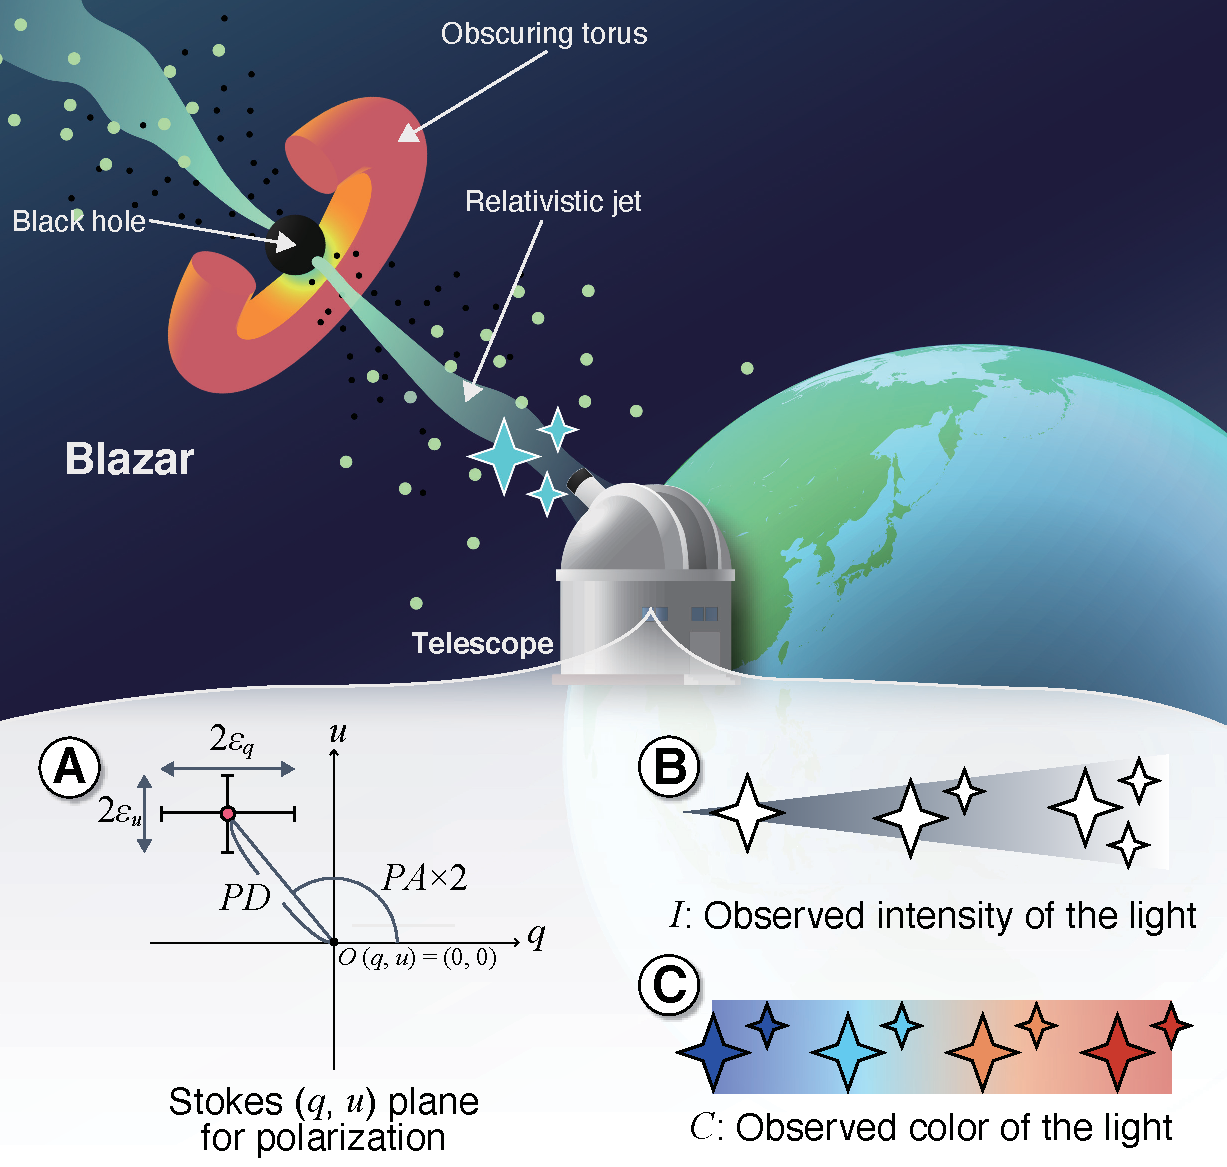
\includegraphics[width=.99\linewidth]{vgtc_journal_latex/figures/blazar_final.pdf}
    \caption{Observed blazar and its features. A blazar's central black hole emits a relativistic jet toward the Earth.
        The telescope observes its light in terms of (A) polarization, (B) intensity, and (C) color.}
    \label{fig:blazar}
\end{figure}

\subsection{Goals and Visualization Tasks}\label{sec:domainGoalsandTasks}
% \begin{figure}[tb]
%     \centering
%     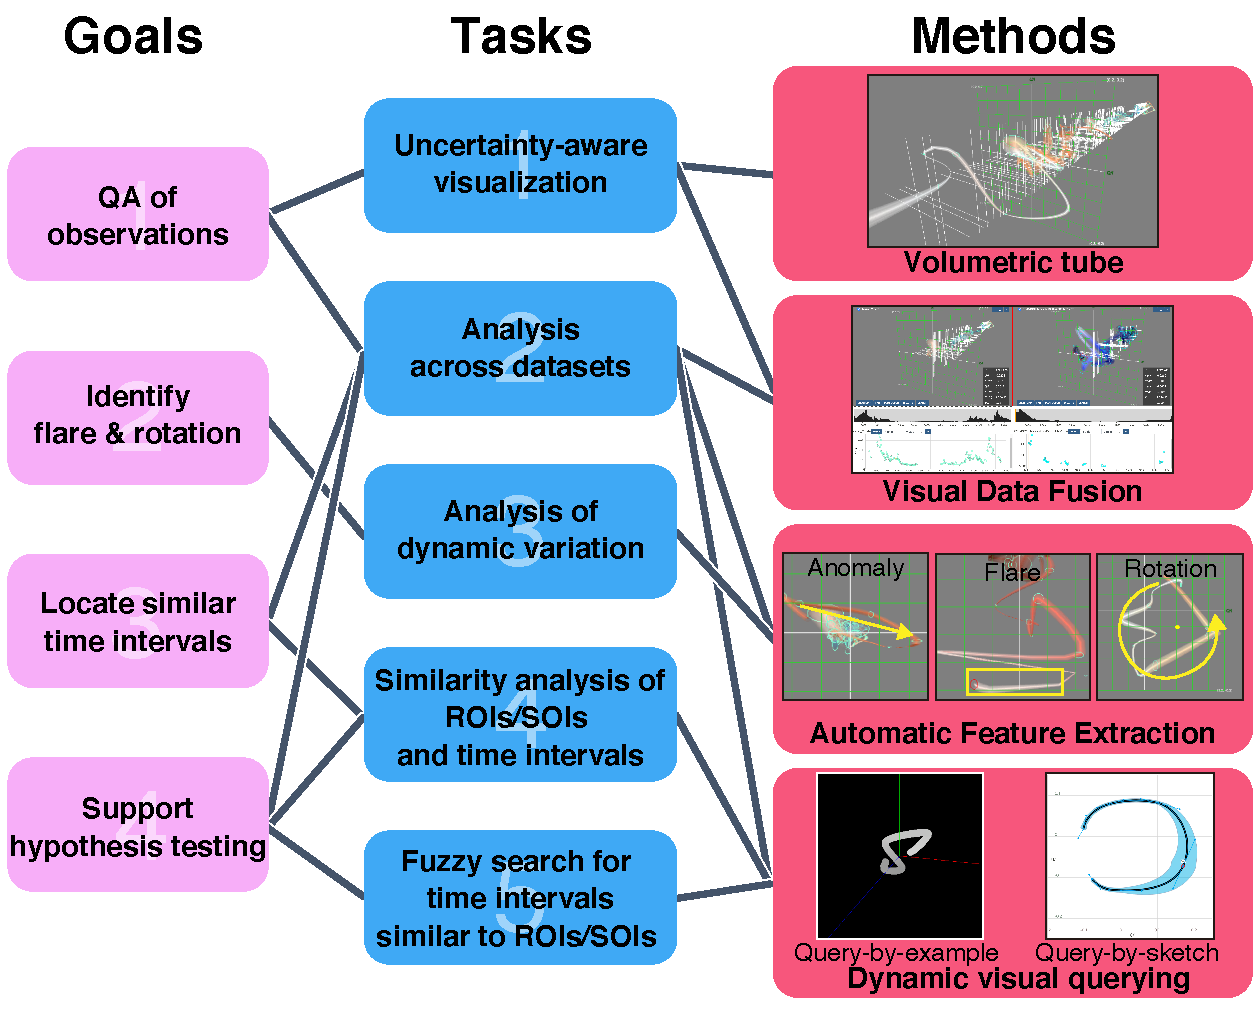
\includegraphics[width=.99\linewidth]{vgtc_journal_latex/figures/many-to-many.pdf}
%     \caption{Mapping of four domain goals, five time-series data analysis tasks, and four functions of TimeTubesX.}
%     \label{fig:mapping}
% \end{figure}
We interviewed two astronomers at Hiroshima University, one at Stanford University, and four at Boston University to clarify domain goals and visualization tasks.
% which has nine blazar researchers.
The main objective of these astronomers is 
to quickly extract and analyze features in temporal variations of observed polarization, intensity, and color that are occurring in multiple time intervals. 
TimeTubesX effectively supports the following four domain goals:

\noindent\textbf{G1--Enhance the reliability of blazar observations}. 
% Due to the rotation of the Earth or bad atmospheric conditions, 
Datasets always contain missing data and observation errors. 
Astronomers need to assess what they found is plausible by analyzing the length of missing data periods and the size of errors.

\noindent\textbf{G2--Identify flares and rotations}. 
Astronomers typically pay attention to time intervals with dynamic time variations, %features that dynamically change over a period of time. 
% Examples include 
such as flares and rotations.
% such as flares that occur when the blazar is more energetic than usual and polarization rotations. %, which sometimes co-occur with dynamic changes of $I$ or $C$.
The analysis of time intervals with such dynamic variations helps astronomers demystify the jet's structures.
% For example, astronomers are interested in polarization variations at the time of flares.
% These dynamic behaviors are important because they help astronomers demystify the jet's structures.

\noindent\textbf{G3--Locate recurring blazar behaviors}.
Besides well-known behaviors such as flares and rotations, 
recurring patterns or common features can also exist.
Thus, finding an interesting pattern or feature, 
astronomers want to locate other time intervals similar to it.

\noindent\textbf{G4--Explore time intervals validating a hypothesis of blazar behaviors}.
Through their analyses or experiences, astronomers sometimes make a hypothesis, e.g., the flares of a blazar tend to co-occur with a specific polarization variation pattern. 
Astronomers need to address time intervals that might validate the hypothesis.

% \begin{enumerate}[nosep, label=\textbf{G\arabic*}, align=parleft, leftmargin=*]
%     \item Enhance the reliability of observations;
%     \item Identify flares and rotations;
%     \item Locate time intervals similar to a specific region/shape of interest (\textit{ROI} or \textit{SOI});
%     \item Explore time intervals validating specific hypotheses.
% \end{enumerate}

To reach these goals, we have identified five visualization tasks that TimeTubesX should support:

\noindent\textbf{T1--Uncertainty-aware visualization.} 
% Due to bad atmospheric conditions or the rotation of the Earth, datasets will always contain observation errors and missing data. 
% Astronomers need to assess whether the interesting behavior they found is plausible or not by analyzing the size of observation errors and the length of missing data periods.
Users should be able to perceive the reliability of data through visualizations. 

\noindent\textbf{T2--Analysis across datasets.} 
% Combining datasets from multiple observatories can reduce the effect of observation errors and compensate for missing data. 
% Additionally, some astronomers want to extract features over several datasets.
%On the other hand, some astronomers think there can exist a universal feature among multiple blazars.
To compensate for missing data, 
the system has to allow users to aggregate datasets for the same target from different sources.
Analyses across datasets should also be supported to address features common to multiple targets.

\noindent\textbf{T3--Analysis of dynamic variations.} 
% Astronomers typically want to identify time intervals with dynamic changes. %features that dynamically change over a period of time. 
% Examples include flares, when the blazar is more energetic than usual, or polarization rotations, which sometimes co-occur with dynamic changes of $I$ or $C$.
Time intervals with drastic changes in a short time period and those with unusual large time variations should be automatically extracted.
% Users want to investigate drastic temporal changes over a few days and large changes in values.
% or a sudden change in the polarization angle.
%The rotation of polarization is also interesting to them. 
% Some astronomers think rotations tend to co-occur with dynamic changes of $I$ or $C$. 
% Thus, TimeTubesX supports the analysis of dynamic variations of polarization, intensity, and color by incorporating different feature extraction on querying methods. %can be observable blazar behaviors.

\noindent\textbf{T4--Similarity analysis of a specific region/shape of interest and time intervals.} 
% When finding an interesting pattern, 
% % When finding an interesting behavior/pattern or confirming a hypothesis, 
% astronomers want to find other time intervals similar to the pattern. 
% This requires the ability not only to identify ROIs/SOIs, but also to search for similar data points.
% , either by the automatic feature detection or dynamic visual queries.
Users should be able to identify regions/shapes of interest (\emph{ROI}s/\emph{SOI}s) and search for similar time variation patterns in other time intervals without complex query languages or parameter settings.
% The system should allow users to build a query for a ROI/SOI without complex query languages or parameter settings.

\noindent\textbf{T5--Fuzzy search for time intervals similar to a ROI/SOI.}
%A prerequisite for similarity analysis between similar time intervals is the ability to detect similar intervals.
%Astronomers are not only interested in finding highly similar time intervals, 
% Astronomers are interested not only in exact matches between a ROI/SOI and similar time intervals, but also in fuzzy or approximate matches. 
% For example, they need to find time intervals that have similar time variations to the ROI/SOI, but are in a different scale or at a different position on the Stokes plane.
% A single query can be produced under different mental models.
The system should provide not only exact matches between a ROI/SOI and time intervals but also fuzzy or approximate matches. 
%There exist time intervals which have similar time variations but in a different scale or at different position on the Stokes plane. 
%The astronomers want to distinguish among these.

% Our previous work~\cite{Fujishiro2018}, TimeTubes, has already supported the first two tasks.
% To support \textbf{G1},
% we have proposed the 3D volumetric tube visualization,
% which allows users to perceive uncertainties of observations (\textbf{T1}).
% % The volumetric tube visualization itself makes users perceive uncertainties of observations (\textbf{T1}). 
% The vagueness of the tube's appearance allows users to recognize the reliability of data samples.
% An ellipsoidal snapshot and a white cruciform axis appear at each observation time stamp to distinguish missing data.
% To ameliorate the ambiguities caused by missing data or observation errors (\textbf{G1}), we have introduced the visual data fusion, which allows users not only to aggregate multiple datasets for the same blazar but also to effectively compare multiple datasets for the same/different blazar in a single visualization session (\textbf{T2}).
% To achieve the remaining goals (\textbf{G2}, \textbf{G3}, \textbf{G4}),
% TimeTubesX also supports \textbf{T3}, \textbf{T4}, and \textbf{T5} by incorporating automatic feature extraction and dynamic visual querying.
% , as we will explain in the rest of the paper.
To support \textbf{G1}, our previous work, TimeTubes~\cite{Fujishiro2018}, has already supported \textbf{T1} and \textbf{T2}.
Observations errors are encoded in the appearance of the 3D volumetric tube (\textbf{T1}).
An ellipsoidal snapshot and a white cruciform axis appear at each observation time stamp to distinguish missing data (\textbf{T1}).
Analysis across datasets (\textbf{T2}) is supported by visual data fusion, which allows users not only to aggregate multiple datasets for the same blazar but also to effectively compare multiple datasets for the same/different blazar in a single visualization session.
In this paper, we mainly focus on feature and pattern detection methods to support the remaining tasks (\textbf{T3}, \textbf{T4}, \textbf{T5}).
Consequently, we have designed an integrated visual analytics framework for blazar observations that supports all identified goals (\textbf{G1} - \textbf{G4}) and tasks (\textbf{T1} - \textbf{T5}).


% So, they want to query ROI or test their hypothesis across datasets for multiple different blazars.
% If they can find such time variations, the behavior or hypothesis can be reported as a new feature.
% ROI querying

% \textbf{T3 -- Hypothesis test.} Universality between behaviors is the most important factor for astronomers. 
% Through their analyses or experiences, they sometimes build a hypothesis. 
% To verify the hypothesis, they scrutinize time intervals satisfying it.
% Their shapes look similar but inherently different. 
% Time variations of data samples on the Stokes plane are affected by other polarization components in the universe. 
% There can exist time intervals with a similar shape to other time interval but in the different position of the Stoke plane.
% The position of the rotation center is not consistent. 
% For example, one rotation starting from the origin of the Stoke plane may move to the upper right and then come back to the origin in a counterclockwise direction, 
% while other rotation starting from the origin of the Stoke plane may move to the lower left and then come back to the origin in a counterclockwise direction.
% Their shapes look similar but inherently different. 
% The astronomers want to distinguish between these.
% To efficiently complete the remaining tasks,
% users have to analyze the spatial and color variation of the 3D tube meticulously even with the previous version of TimeTubes.
\section{System Design\label{sec:systemDesign}}
In this section, we provide an overview of visual encoding for blazar data and the visual exploration framework of TimeTubesX.
% We introduce a 3D tube expression of our previous TimeTubes~\cite{Fujishiro2018} into TimeTubesX.

\begin{figure}[tb]
    \begin{minipage}{0.34\linewidth}
        \centering
        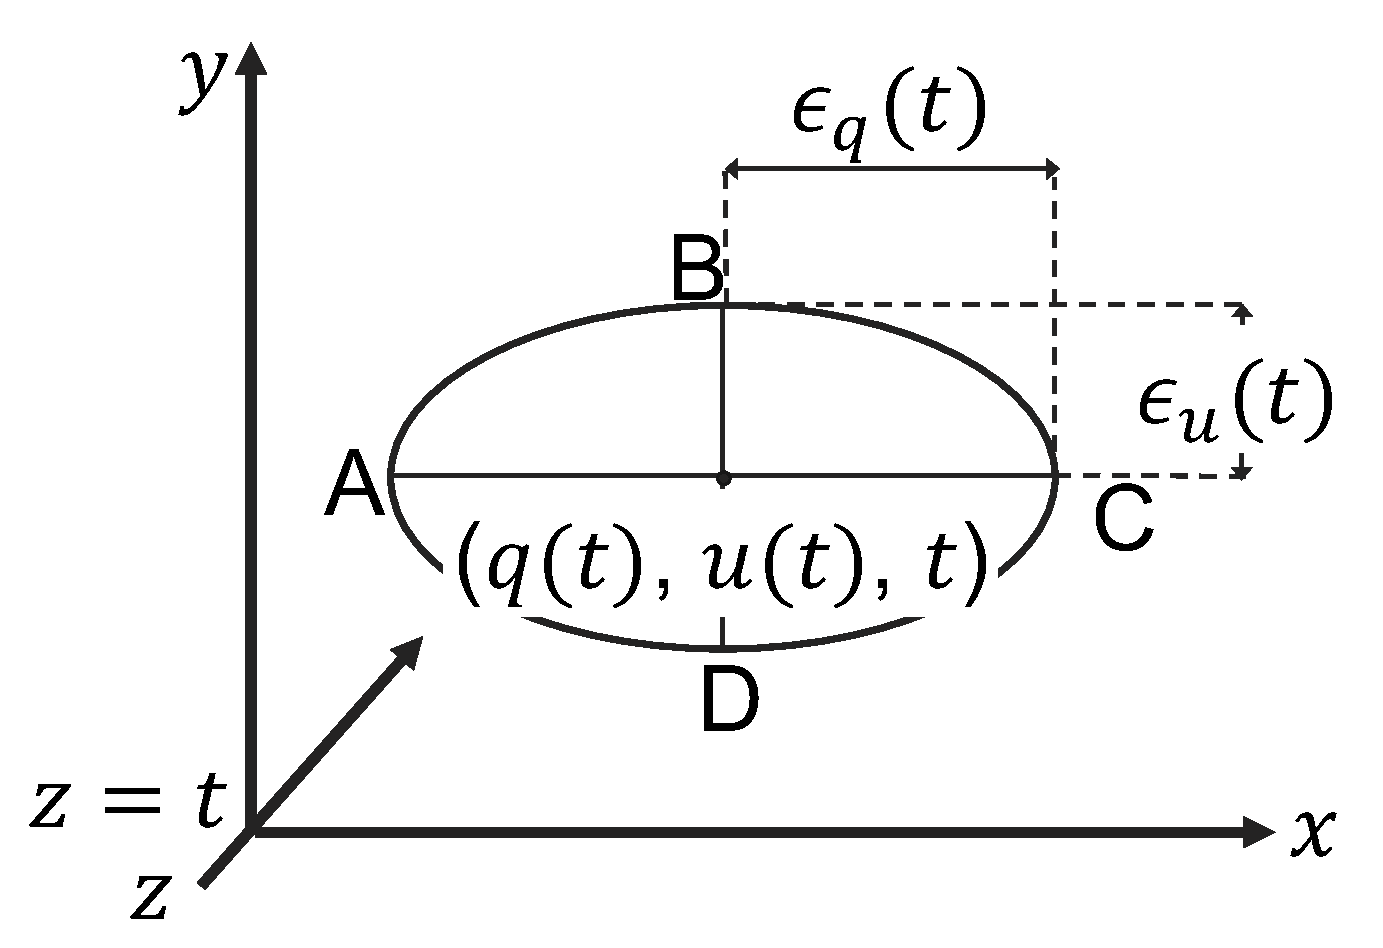
\includegraphics[width=.99\linewidth]{vgtc_journal_latex/figures/howtoplot.pdf}
    \end{minipage}
    \begin{minipage}{0.26\linewidth}
        \centering
        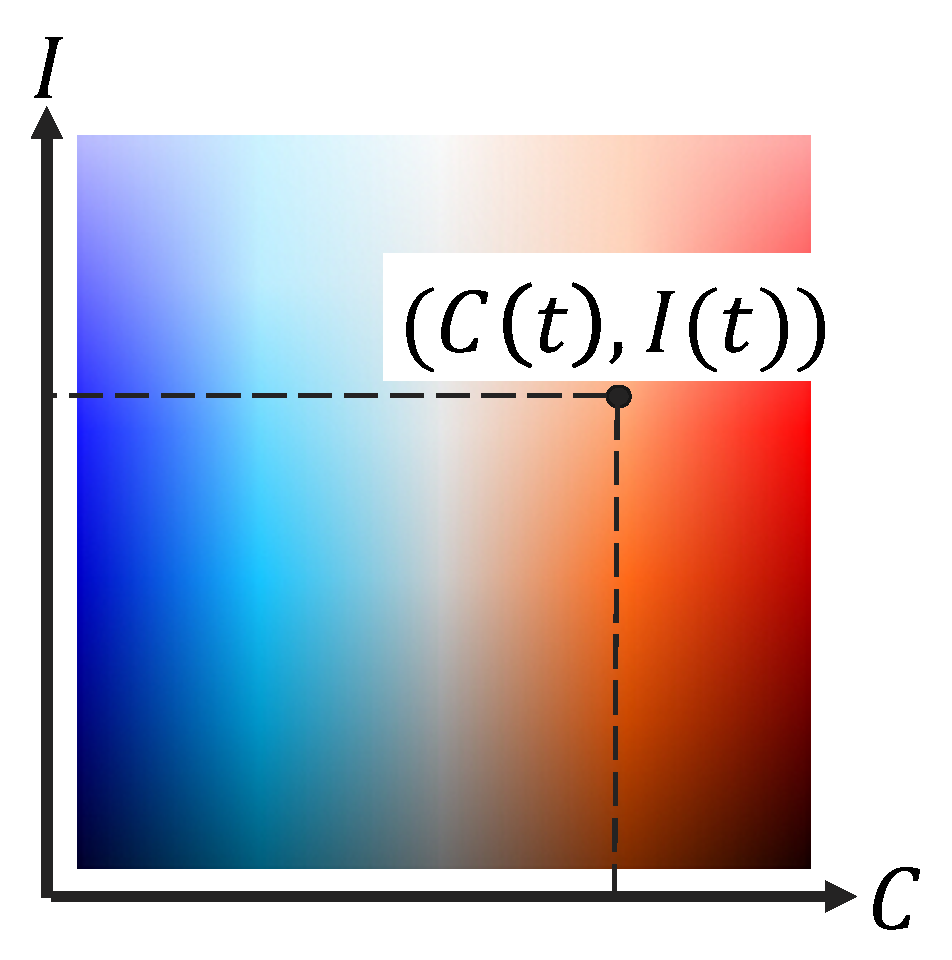
\includegraphics[width=.99\linewidth]{vgtc_journal_latex/figures/colormap.pdf}
    \end{minipage}
    \begin{minipage}{0.36\linewidth}
        \centering
        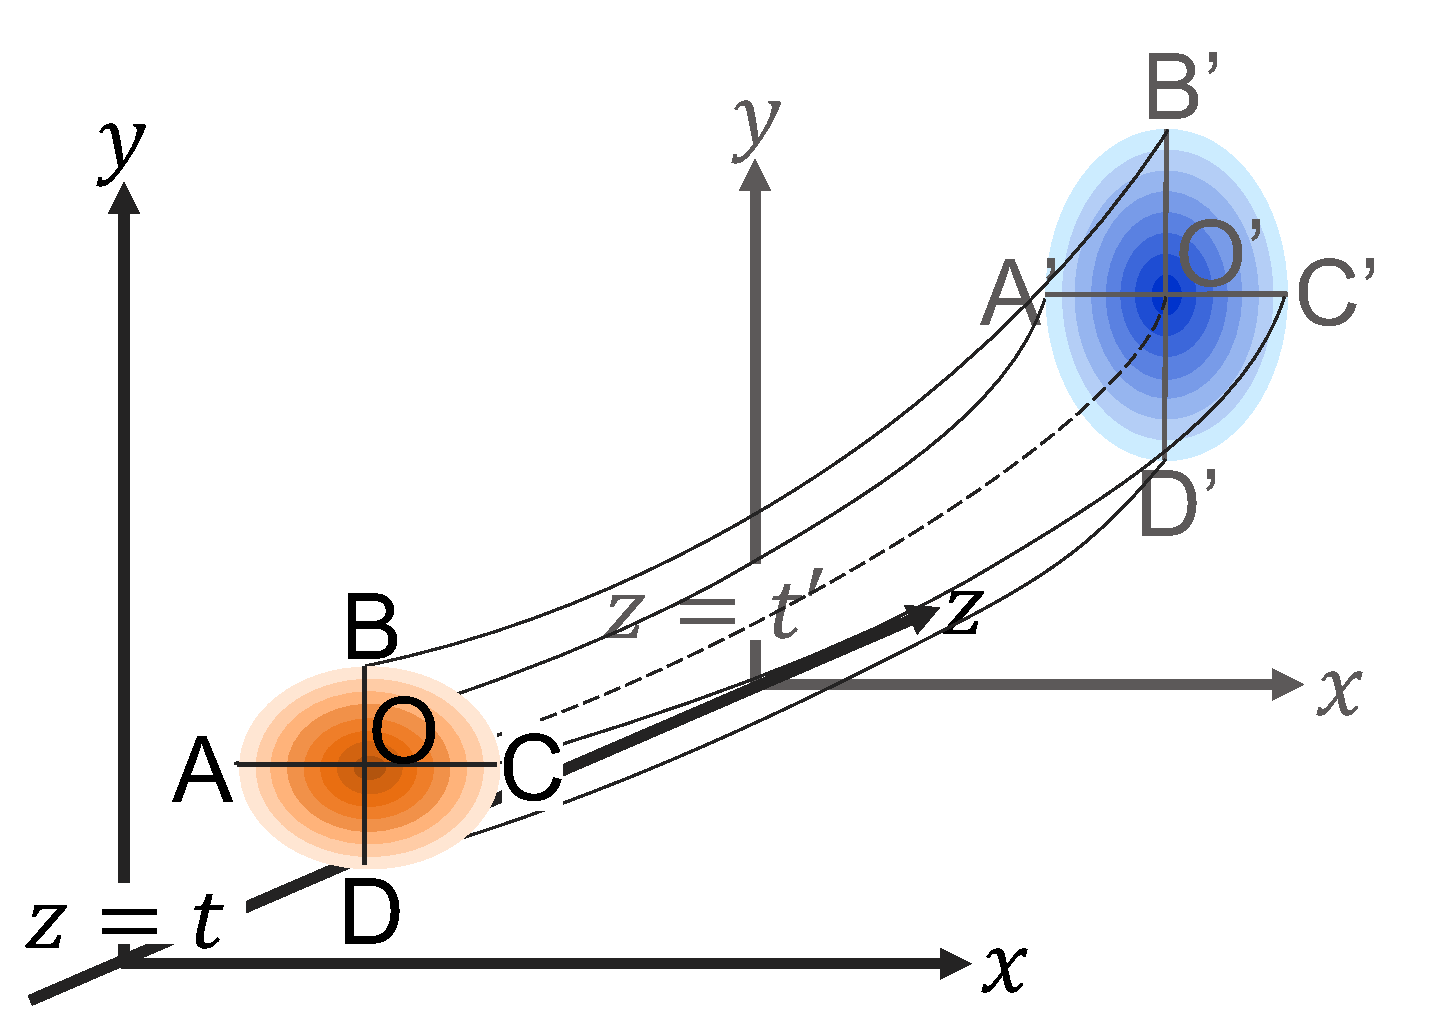
\includegraphics[width=.99\linewidth]{vgtc_journal_latex/figures/howtotube.pdf}
    \end{minipage}
    \begin{minipage}{0.34\linewidth}
        \centering
        \footnotesize{\sf (a)}
        \end{minipage}
    \begin{minipage}{0.26\linewidth}
        \centering
        \footnotesize{\sf (b)}
    \end{minipage}
    \begin{minipage}{0.36\linewidth}
        \centering
        \footnotesize{\sf (c)}
    \end{minipage}
    \caption{Spatial mapping in the TimeTubes view. 
    (a)~Observation values of polarization decide the position and shape of an ellipse;
    (b)~observation values of intensity and color colorize the ellipse with reference to a colormap; and
    (c)~the neighboring ellipses are smoothly connected in chronological order to yield a tube shape.}
    \label{fig:howtoplot}
\end{figure}
\subsection{Visual Encoding for Blazar Data}\label{sec:VisualEncoding}
\begin{figure*}
    \centering
    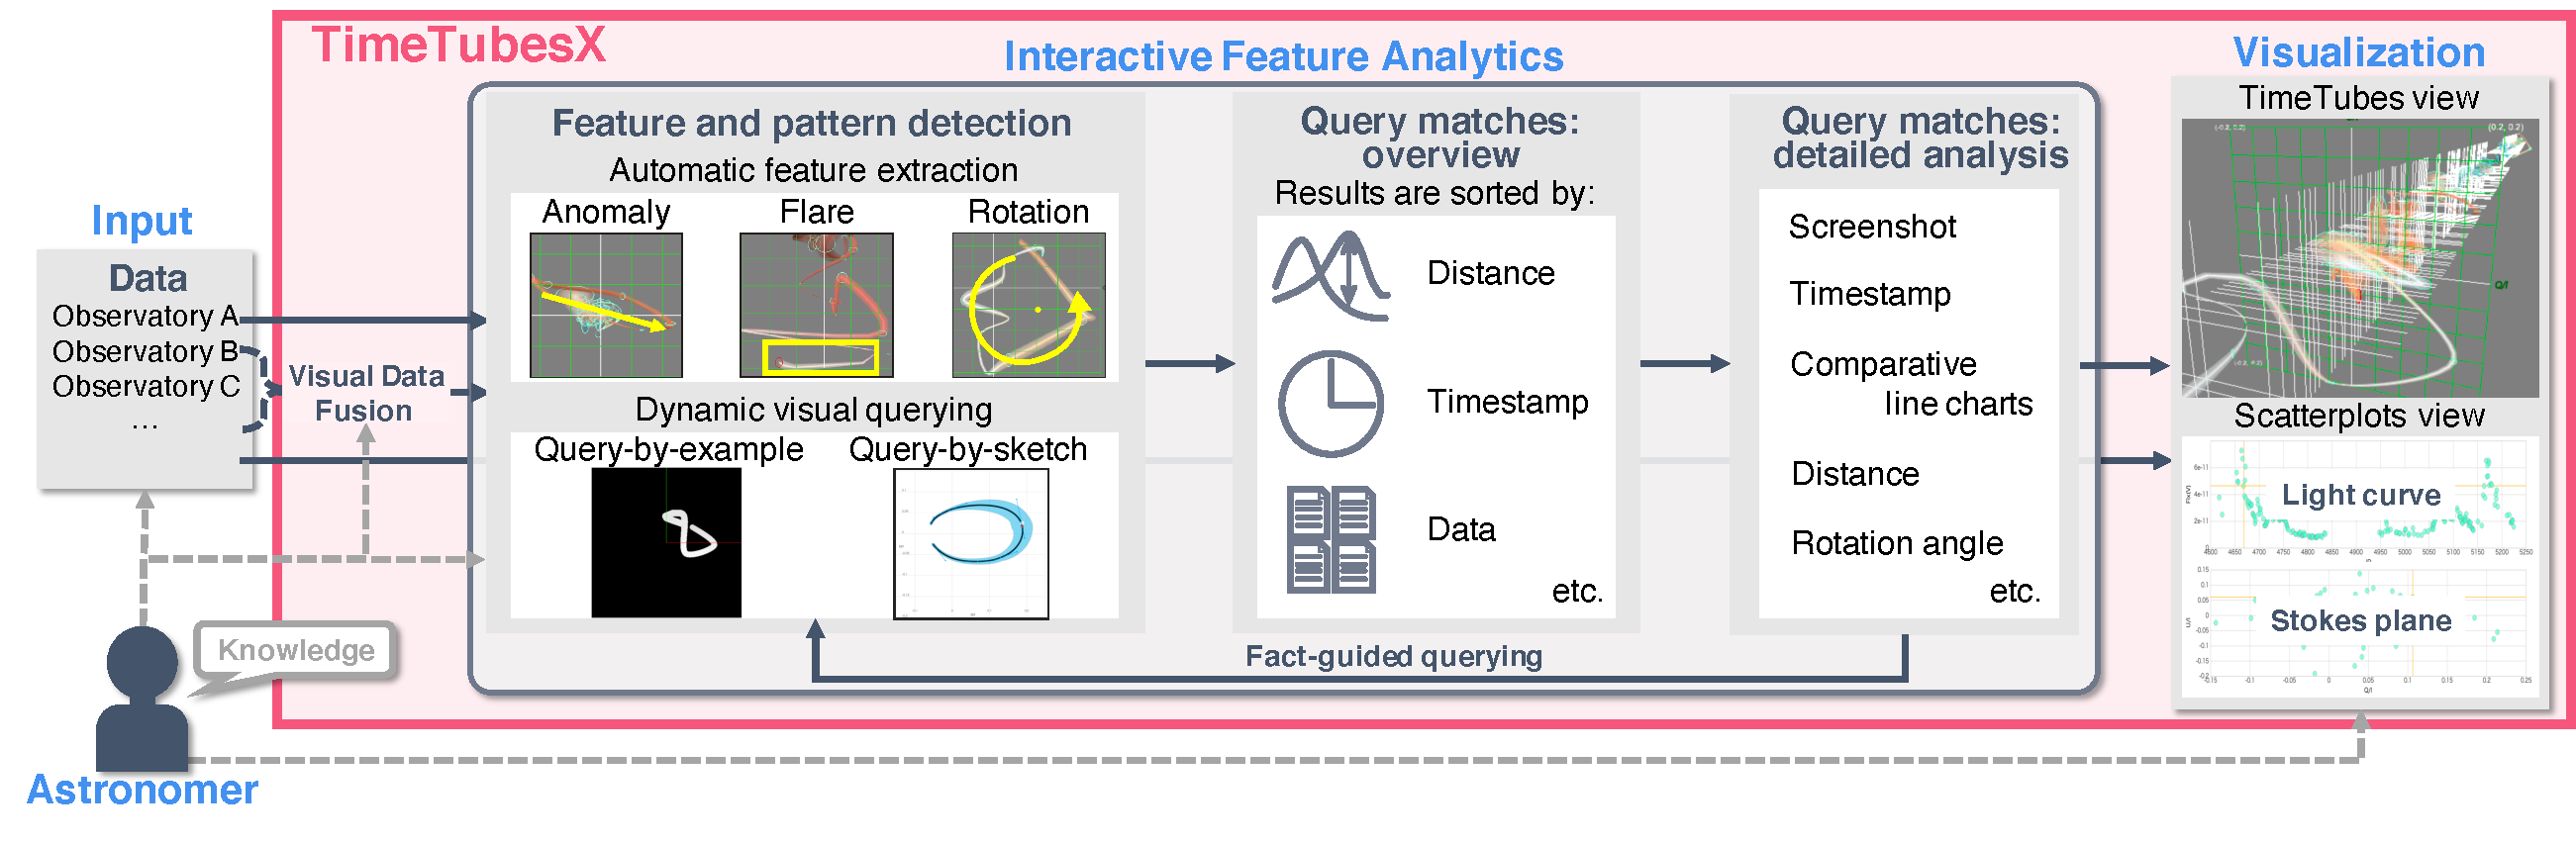
\includegraphics[width=.99\linewidth]{vgtc_journal_latex/figures/workflowGray.pdf}
    \caption{The visual exploration framework of TimeTubesX. Users can load multiple datasets into a single exploration session through visual data fusion. (A)~Users specify a query to extract features of interest; (B)~query results are sorted by relevance; (C)~individual results can be analyzed in high detail and compared to each other; (D)~an extraction result can be re-used as an input for a new visual query; and (E)~users can visually explore the results in the TimeTubes and scatterplots views.}
    \label{fig:framework}
\end{figure*}
Astronomers have used three animated scatterplots with error bars to visualize their multi-dimensional, time-dependent observations (see the accompanying video): one for time variation of $I$, termed \textit{light curve}, another for the Stokes plane, and a third for the correlation between $I$ and $C$.
During the animation, individual observations are highlighted in red in order of observation.
% The animated scatterplots are comprised of three scatterplots, one for the time variation of $I$, termed \textit{light curve}, another for the Stokes plane, and a third for the correlation between $I$ and $C$.
% The \textit{light curve} (\autoref{fig:traditionalMethod}~(a)) is the most important plot for astronomers, and shows the variation of $I$ over time. 
% (b) shows the Stokes plane,
% while (c) displays the correlation between $I$ and $C$.
%

Instead of animating multiple 2D scatterplots,
TimeTubesX expresses blazar observations as a single 3D volumetric tube. 
In the following part, we give a short overview of the \emph{TimeTubes view}, which was originally proposed in our previous work~\cite{Fujishiro2018}.
% We call the view of the 3D volumetric tube \emph{TimeTubes view}.
The TimeTubes view %, that is explained in Fig.~\ref{fig:howtoplot}, 
allows users to see correlations and variations of variables over time at a glance, as illustrated in Fig.~\ref{fig:framework}~(E).
In the current version, users need to import .csv files with column names from their local environment into TimeTubesX.
%as shown in TimeTubes view in the lower right of \autoref{fig:framework}.
%
We use a left-handed coordinate system to assign $q$ and $u$ to the $x$ and $y$ axes, respectively, and time $t$ to the $z$ axis.
%of the visualization domain, $u$ to $y$ axis, and $t$ to $z$ axis.
We encode the polarization parameters ($q$, $u$, $\epsilon_q$, $\epsilon_u$) at each timestamp $t$ as an ellipse centered at the point $(x, y, z) = (q(t), u(t), t)$ with a width of $2\epsilon_q(t)$ and a height of $2\epsilon_u(t)$, as depicted in Fig.~\ref{fig:howtoplot}~(a). 
Therefore, the $x$--$y$ location of an ellipse indicates the polarization at a certain time stamp, while the size of the ellipse indicates the uncertainty of the measurement.
To properly render a 3D tube, we set the value range of the Stokes plane in the TimeTubes view with reference to the standard deviations of $q$ and $u$ in the datasets. 
In the current TimeTubes view, we empirically map a single day to a single voxel along the $z$ axis.
%
We colorize the ellipses according to $I(t)$ and $C(t)$ as based on a user-defined 2D colormap (Fig.~\ref{fig:howtoplot}~(b)). 
The TimeTubes view connects neighboring ellipses in chronological order, using centripetal Catmull-Rom splines to form a 3D volumetric tube (Fig.~\ref{fig:howtoplot}~(c)). 
To further reflect the reliability of the observations, the TimeTubes view offers an adjustable opacity transfer function.
Multiple concentric tubes with different transparencies (i.e., higher opacities for inner tubes) compose a single tube that allows users to intuitively perceive the uncertainties of observations.
Specifically, a time interval with small errors looks like an opaque tube, whereas a time interval with large errors looks more semi-transparent and fuzzy.

Compared with the initial animated scatterplots,
the TimeTubes view provides more uncertainty-aware visual encoding for the analysis of blazar behaviors (\textbf{T1}).
Astronomers do not need to scrutinize multiple plots to understand correlations between variables
or move sliders back and forth %in time 
to track time variations.

%
% Refer to our previous paper~\cite{Fujishiro2018} for more details about the visual encoding of TimeTubes. % interactive exploration functions. %, which were designed according to Shneiderman's Visual Information Seeking Mantra~\cite{Shneiderman1996}, as illustrated in the lower right part of \autoref{fig:framework}.

% The main idea of TimeTubes is to show multi-dimensional time-dependent data in a single visualization. 
% \begin{figure}[tb]
%     \begin{center}
%         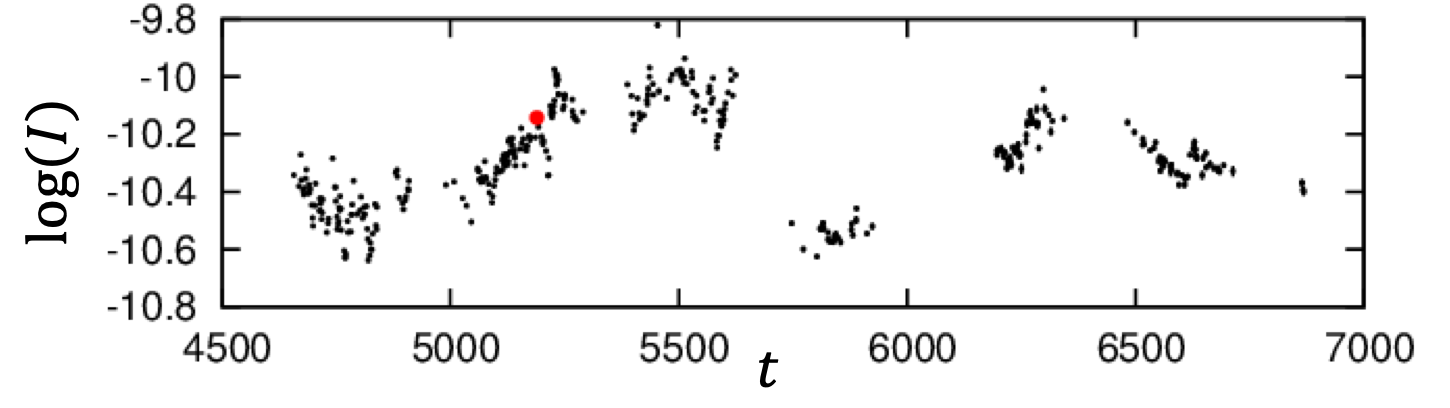
\includegraphics[width=0.75\linewidth]{vgtc_journal_latex/figures/TraditionalMethod_t_I.png}\\
%         \footnotesize{\sf (a)~Light curve ($I$ vs. $t$)}
%     \end{center}
%     \vspace{-5px}
%     \begin{minipage}{0.44\linewidth}
%         \centering
%         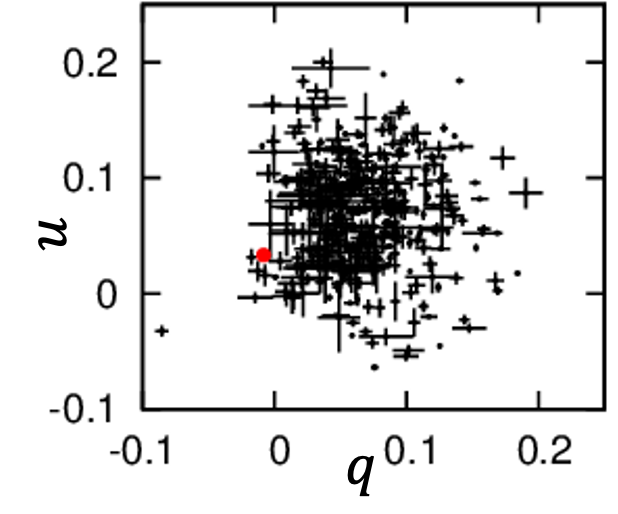
\includegraphics[width=.65\linewidth]{vgtc_journal_latex/figures/TraditionalMethod_q_u.png}\\
%         \footnotesize{\sf (b)~Stokes plane ($u$ vs. $q$)}
%     \end{minipage}
%     \begin{minipage}{0.55\linewidth}
%         \centering
%         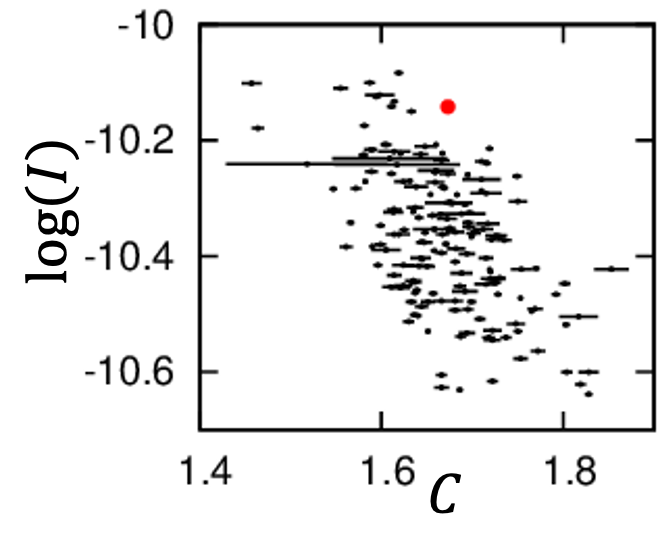
\includegraphics[width=.55\linewidth]{vgtc_journal_latex/figures/TraditionalMethod_c_I.png}\\
%         \footnotesize{\sf (c)~Color–magnitude diagram ($I$ vs. $C$)}
%     \end{minipage}
%     \vspace{-10px}
%     \caption{
%     Animated scatterplots as a conventional way to visualize blazar observations~\cite{Ikejiri2011}. 
%     The plots highlighted in red in sequential order synchronize three scatterplots for cross-reference.
%     }
%     \label{fig:traditionalMethod}
% \end{figure}

\subsection{Visual Exploration Framework\label{sec:approach}}
The design of TimeTubesX supports the visualization tasks outlined in Section~\ref{sec:domainGoalsandTasks}.
Fig.~\ref{fig:framework} illustrates our visual exploration framework.
%
The user workflow starts with visual data fusion~\cite{Fujishiro2018} to create a unified dataset for all subsequent analysis steps (\textbf{T2}).
%All functions can be applied to the unified dataset by visual data fusion~\cite{Fujishiro2018}.
For initial feature and pattern detection (A), users can either rely on automatic feature extraction methods for well-known blazar behaviors (\textbf{T3}) or define their own visual queries for a ROI/SOI (\textbf{T4}, \textbf{T5}).
%For the purpose of the feature extraction, in (A), the user specifies a feature which he/she wants to find out by setting parameters, ROI, or SOI.
The system ranks the results of the feature and pattern detection stage and shows the ranked matches (B).
%the query specified in (A) and shows their overview (B).
Users can sort the results to, for instance, focus on time intervals that have the largest rotation or are the most similar to the input pattern.
%By changing the order of the results, 
%he/she can easily notice which time interval has the biggest rotation 
%or most similar to the input pattern, for instance.
%
% By selecting one or several results of interest, users can analyze, compare, and annotate selected time intervals in more detail (C). 
%By selecting one of the results, he/she may refer to the details of the result and attach an annotation to it if needed (C).
The detailed analysis (C) helps users understand the behavior at the extracted time intervals and classify the results. 
% Annotations allow users to document their analysis process and to share their results with others.
%These details are helpful for him/her understand the the behaviors of the extracted time intervals and
%the annotation supports him/her in recalling his/her analysis process, classify the results, and share the results with other users.
To support iterative refinement of queries, users can build a follow-up query based on the result of a query (D). It allows users to find time intervals similar to the result (\textbf{T4}).
%for another query in the next interactive feature extraction phase (D).
We call this \textit{fact-guided querying}, as it enables users to refine extraction results guided by previously detected features.
To analyze extracted time intervals in more detail, users can employ
the uncertainty-aware TimeTubes view (\textbf{T1}) as well as multiple linked scatterplots views (E).
%He/she can refer to the TimeTubes view as well as the conventional scatterplots view for the extracted time interval with simple interactions (E).
% Our framework supports scatterplots of any two user-defined variables. %, and is linked to the TimeTubes view.
%TimeTubesX can show as many kinds of scatterplots between two arbitrary variables as he/she likes, 
%any of which are federated with TimeTubes view.
%It allows him/her to obtain knowledge or insights on the blazar behaviors.

\textsf{Interactive feature analysis interface.\ } 
% One of the main contributions of TimeTubesX lies in the inherent support for the automatic feature extraction and dynamic visual querying for multi-dimensional, time-dependent blazar datasets.
Fig.~\ref{fig:UIFeatureExtraction} shows our feature and pattern detection user interface. 
The query specification panel (A) allows users %to specify what to extract and 
to build a query with simple interactions either by selecting what to extract, picking a part of data as an input, or sketching time variation patterns.
% In \autoref{fig:UIFeatureExtraction}, (A) shows an on-going query-by-sketch user interaction.
After running a similarity search, 
TimeTubesX ranks and filters extraction results according to the parameters in panel (B),
and then it displays all relevant (i.e., non-filtered) extraction results as a collection of thumbnails in panel (E).
The distance distribution histogram in panel (B) helps users to further filter the number of results.
% which allows users to sort results and to set thresholds for further filtering the number of displayed results.
% To help users set filtering thresholds,
% we use a histogram to provide an overview of the distribution of distances returned by the similarity search.
% By adjusting the gray area on the histogram, users are allowed to alter the number of displayed results. 
The timeline in panel (C) gives an overview of the temporal distribution of the results.
Users are able to recognize groups of results sharing identical time points and temporal distribution features.
% The thumbnails of all relevant (i.e., non-filtered) results are shown in panel (E) to give users an intuitive overview of their query results.
When selecting an individual thumbnail, TimeTubesX shows a detailed information on the corresponding result in panel (D), including exact time stamps and the distance between the query and the result.
% The detailed information is helpful for users' deeper understanding of the extracted time interval.
To re-utilize the query, compare multiple query results, and share the query and their results with other users, 
TimeTubesX allows users to export and import queries and their results in the form of JSON files (a custom format for TimeTubesX).
When importing previous query results,
panel (F) shows a summary of the query used in the previous process and panel (C) shows another timeline for the imported query results.

Fig.~\ref{fig:querySpecificationPanel} shows the query specification panels for each mode of the feature and pattern detection.

% MERGED VERSION
% The design of TimeTubesX supports the visualization tasks outlined in \autoref{sec:domainGoalsandTasks}.
% \autoref{fig:framework} illustrates our visual exploration framework, while \autoref{fig:UIFeatureExtraction} shows our feature and pattern detection user interface.
% The visual exploration workflow starts with visual data fusion~\cite{Fujishiro2018} to create a unified dataset for all subsequent analysis steps (\textbf{T2}).
% For initial feature and pattern detection in \autoref{fig:framework}~(A), users can either rely on automatic feature extraction methods for well-known blazar behaviors (\textbf{T3}) or can define their own visual queries for a ROI/SOI (\textbf{T4}, \textbf{T5}).
% The query specification panel in \autoref{fig:UIFeatureExtraction}~(A) allows users to specify what to extract and to build a query with simple interactions.
% As the next step, the system ranks the results of the feature and pattern detection stage and shows the ranked matches, as illustrated in  \autoref{fig:framework}~(B).
% Users can sort the results, e.g., to focus on time intervals that have the largest rotation or are the most similar to the input pattern.
% They are allowed to choose in what order to sort the results and set thresholds for further filtering the number of displayed results with the suggestion of a distance distribution histogram in \autoref{fig:UIFeatureExtraction}~(B).
% % By adjusting the gray area on the histogram, users are allowed to alter the number of displayed results.
% They can overview the temporal distribution of all relevant (i.e., non-filtered) extraction results through the timelines in \autoref{fig:UIFeatureExtraction}~(C) and the thumbnails of sorted results in \autoref{fig:UIFeatureExtraction}~(E).
% The detailed analysis in \autoref{fig:framework}~(C) helps users deeply understand the behavior of the extracted time intervals and classify their results. 
% \autoref{fig:UIFeatureExtraction}~(D) shows detailed information on a selected result, including exact time stamps and the distance between the query and the result.
% To support iterative refinement of queries, users can build a follow-up query based on the result of a query, as illustrated in \autoref{fig:framework}~(D). 
% It allows users to identify time intervals similar to the result (\textbf{T4}).
% We call this \textit{fact-guided querying}, as it enables users to refine extraction results guided by previously detected features.
% To analyze extracted time intervals in more detail, users can employ
% the uncertainty-aware TimeTubes view (\textbf{T1}) as well as multiple linked scatterplots views, as shown in \autoref{fig:framework}~(E).
% Our framework supports scatterplots of any two user-defined variables. 
% To compare multiple query results,
% TimeTubesX allows users to export and import query results.
% When importing previous query results,
% \autoref{fig:UIFeatureExtraction}~(F) shows a summary of the query used in the previous extraction process, and \autoref{fig:UIFeatureExtraction}~(C) shows another timeline for the imported query results.

To better demonstrate our feature and pattern detection methods, we will use a synthetic dataset (see Fig.~\ref{fig:synthesisData}) as a running example in Sections~\ref{sec:automaticExtraction} and \ref{sec:visualQuery}.
%for illuminating the feature extraction, as illustrated in \autoref{fig:synthesisData}.
It contains four large peaks in $I$, as highlighted by orange diamonds in (a), three small red circular patterns on the Stokes plane in (b), three large green rotations , and three narrow/rough-edged blue patterns.

% \begin{figure}[H]
%     \centering
%     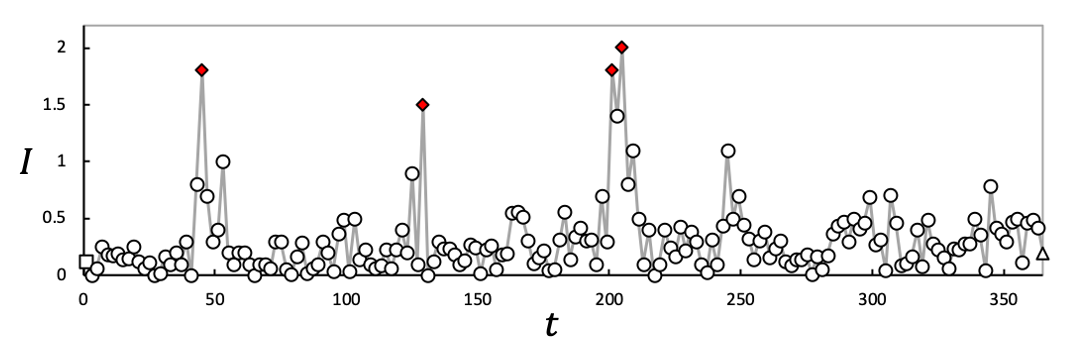
\includegraphics[width=.8\linewidth]{vgtc_journal_latex/figures/synthesisDataLightCurveLabel.png}\\
%     \footnotesize{\sf (a) Light curve plot. The four red diamonds indicate peaks in the data.}\\
%     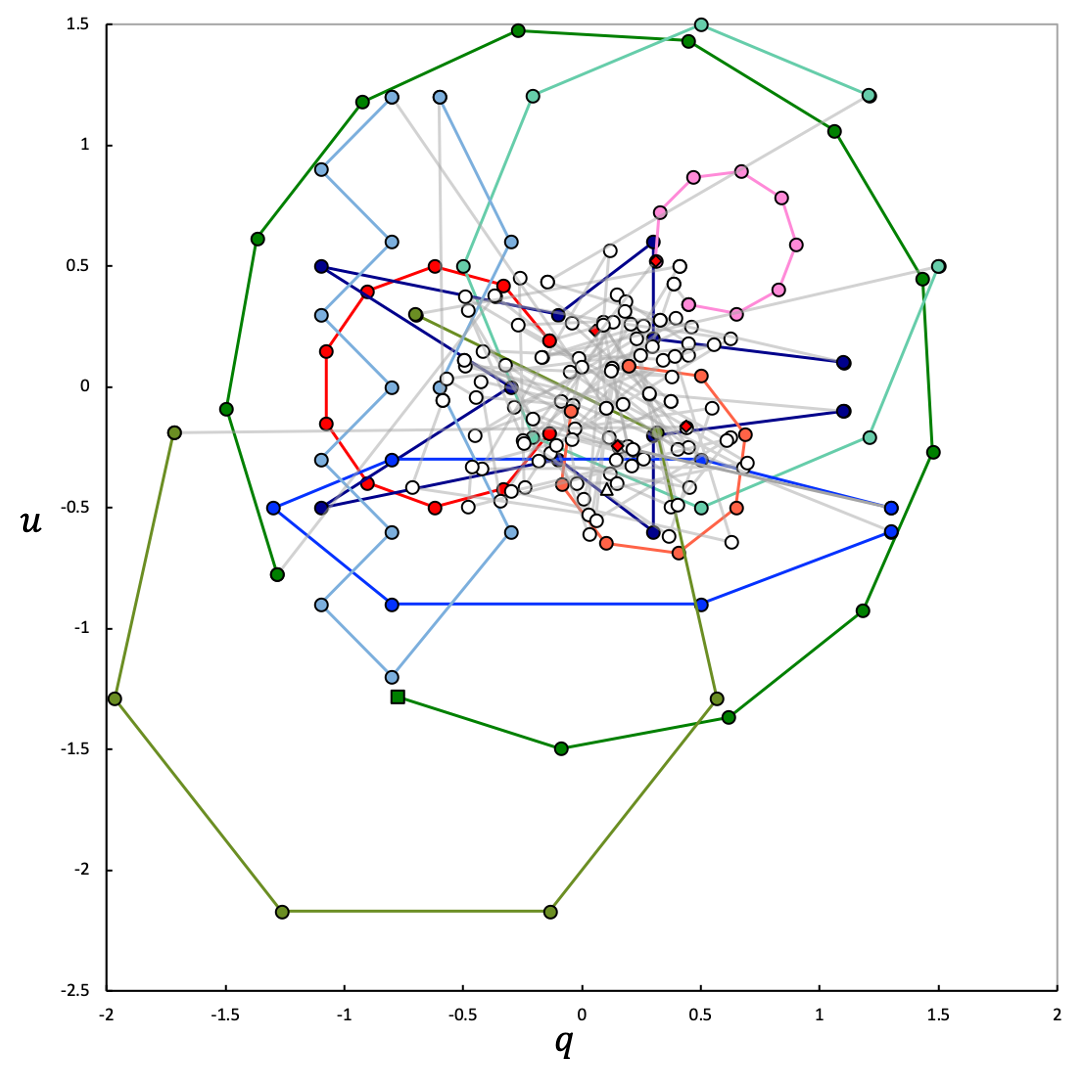
\includegraphics[width=.83\linewidth]{vgtc_journal_latex/figures/synthesisDataStokesLabel.png}\\
%     \footnotesize{\sf (b) Stokes plane plot. The red diamonds indicate the peaks shown in (a).}
%     \caption{Conventional stokes plane and light curve plots for our synthetic dataset. The data includes three small circular patterns (red), three big rotations (green), and three narrow/rough-edged patterns (blue) within 365 days. Data starts from a square plot and ends at a triangular plot.}
%     \label{fig:synthesisData}
% \end{figure}


% \begin{figure*}[t]
%     \centering
%     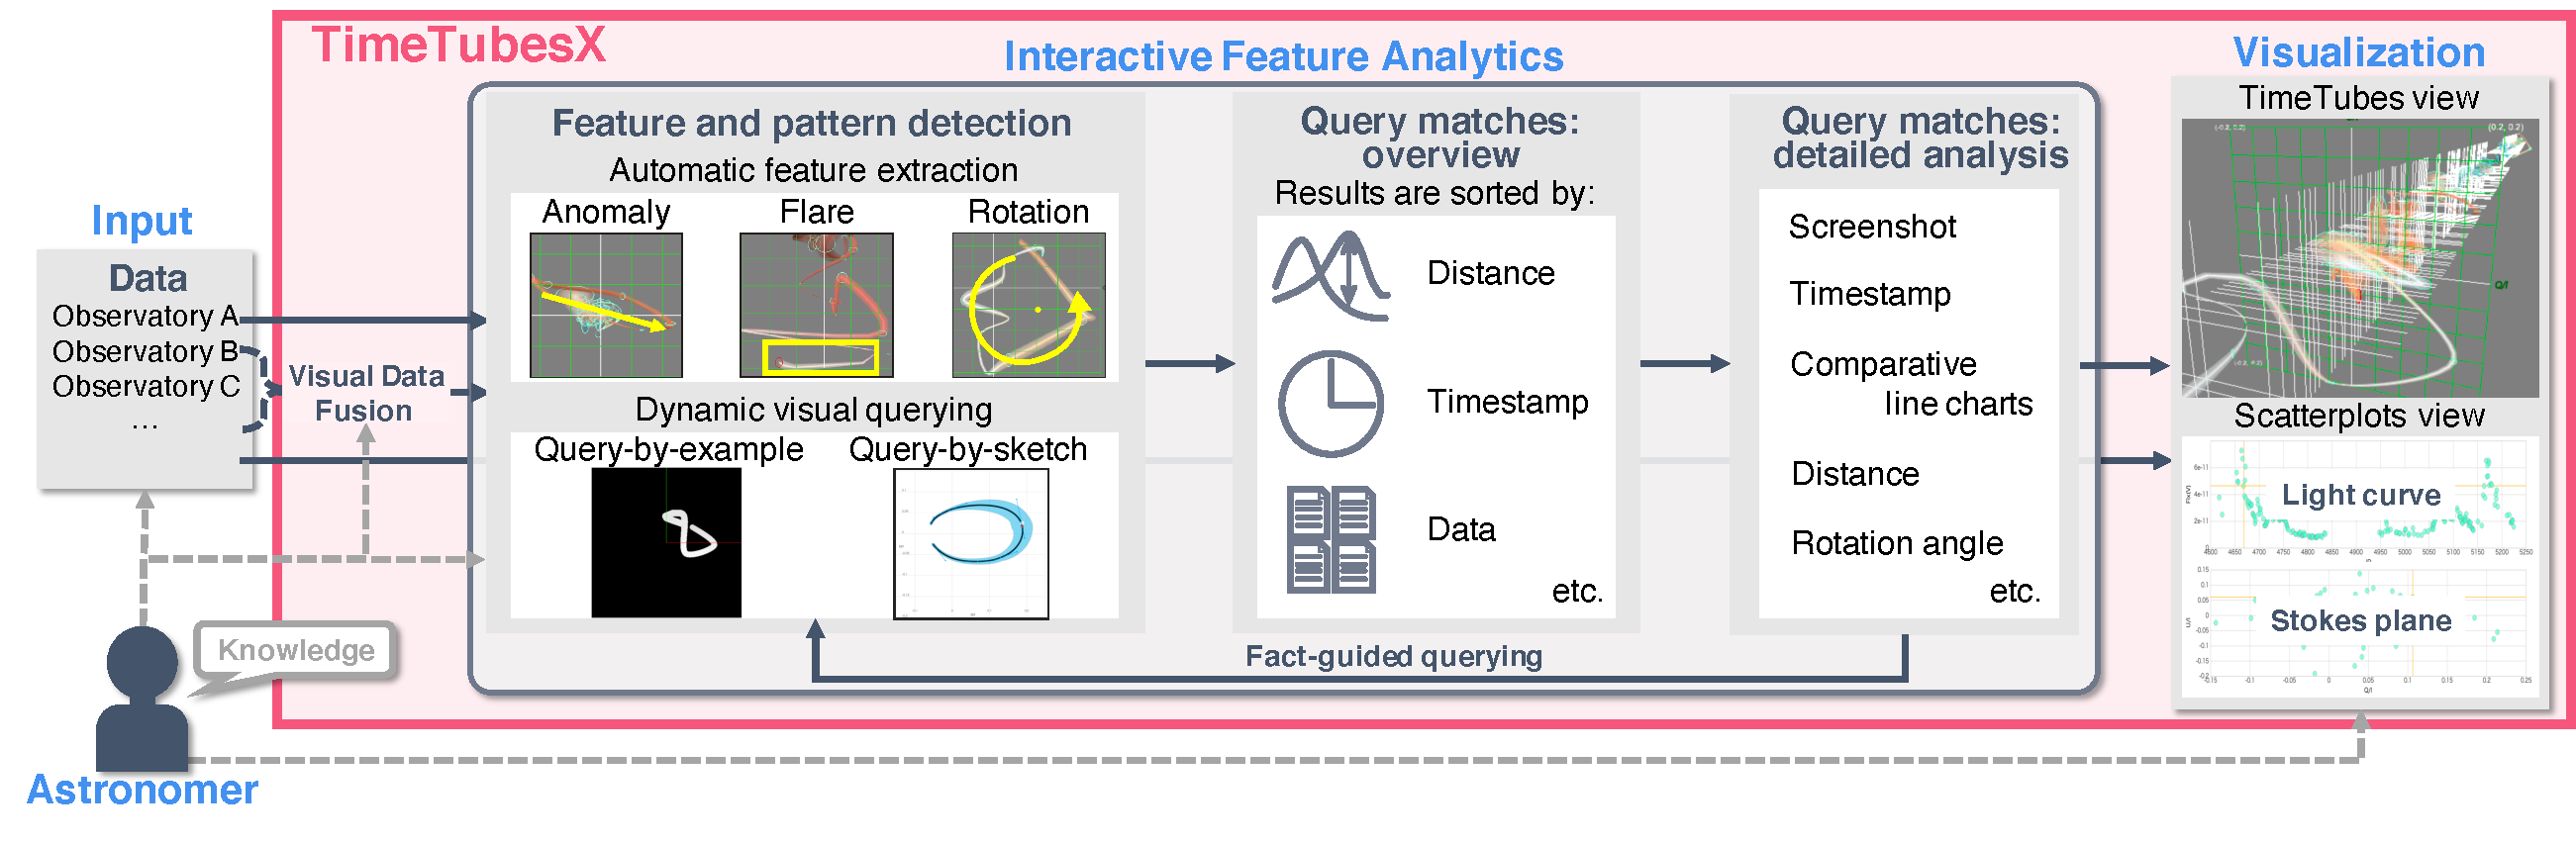
\includegraphics[width=0.9\textwidth]{vgtc_journal_latex/figures/workflowGray.pdf}
%     \caption{Visual exploration framework of TimeTubesX. TimeTubesX can deal with multiple input datasets through visual data fusion. (A)~The user specifies what to extract; (B)~Extraction results are ordered by an arbitrary property; (C)~Detailed information of a selected result is provided; (D)~An extracted result can be re-utilized for another query in the interactive feature extraction; (E)~The user is allowed to refer to TimeTubes view or scatterplots view for the extracted time interval and explore it with various exploration functions.}
%     \label{fig:framework}
% \end{figure*}
% We newly introduce two types of feature extraction into TimeTubesX: automatic and interactive.
% The automatic feature extraction can extract notable time intervals to meet given specifications,
% whereas the interactive feature extraction can find out time intervals similar to a given ROI or SOI. 

% TODO: Move the following part to the introduction?
% Regarding the behaviors of blazars, there are a lot of mysterious parts. 
% When the relativistic jet in a blazar forms a burst, the light from a blazar gets highly luminous, that is called a flare. 
% Flare is one of the most characteristic behaviors. 
% Some astronomers report that the polarization direction of the light from blazars sometimes rotates. 
% However, it is controversial in astronomy whether the rotations are real ones or fake ones caused by random variations of polarization.
% To verify polarization rotations, astronomers need to scrutinize correlations among other observation variables. 
% On the other hand, there can exist undiscovered phenomena of blazars. 
% It is significant to explore recurring patterns of time variations or correlations among variables. 
% Nevertheless, deliberate analysis across multiple variables is indispensable.
% To address these difficulties, we introduce a novel feature extraction for blazar observations.
% It supports two types of feature extraction: Automatic extraction and visual query. 
% The automatic extraction can squeeze only observable time intervals from (multiple) long-term observations, 
% whereas the visual query can find time intervals similar to a region of interest (ROI) or shape of interest (POI). 
% The feature extraction can deal with visually fused datasets.

% It allows him/her to deeply understand blazar behaviors and obtain knowledge or insights on them.
% Note that task \textbf{T2} is supported by all the functions of the feature extraction.

% The following sections (Sections~\ref{sec:automaticExtraction}, \ref{sec:visualQuery}, and \ref{sec:otherFunctions}) detail functions involving the feature extraction.
% \input{Sections/result.tex}
% \begin{figure*}[tb]
%     \centering
%     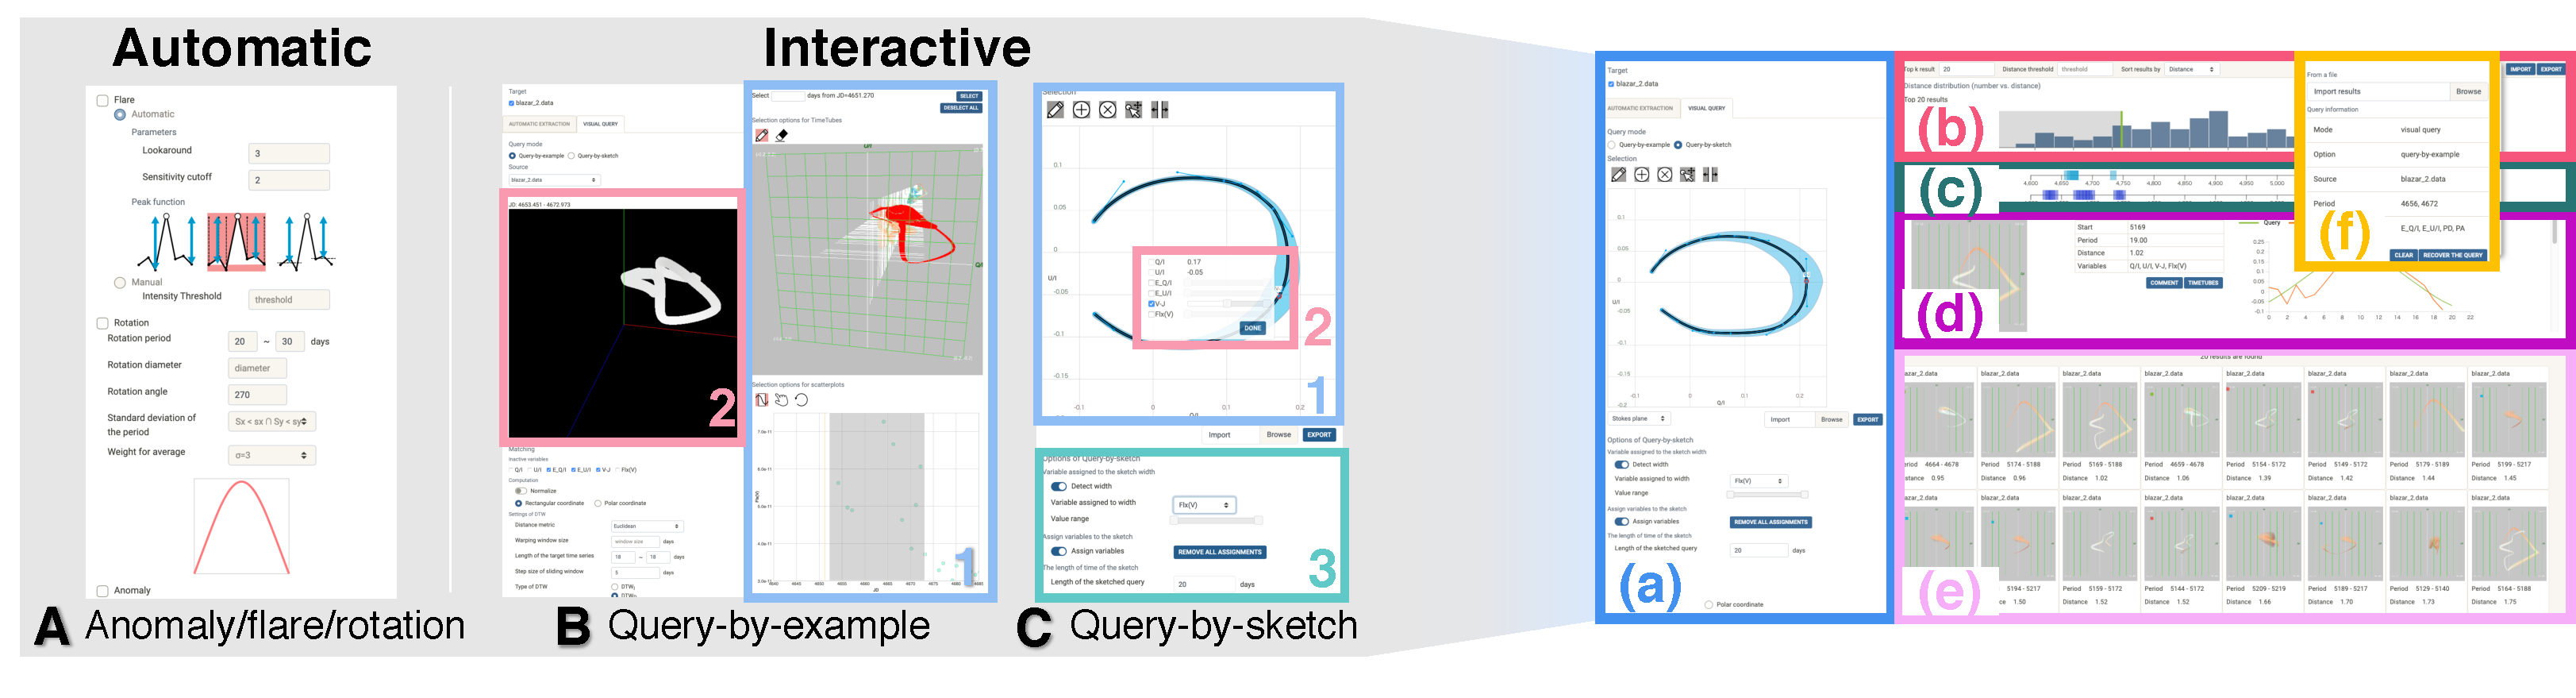
\includegraphics[width=.84\linewidth]{vgtc_journal_latex/figures/GUIwide.pdf}
%     \caption{User interface of the feature extraction. (a)~Query specification panel. The panel with the automatic feature extraction is illustrated in (A), one with query-by-example in (B), and one with query-by-sketch in (C); (b)~Parameters for ranking, filtering, and displaying extraction results and a histogram summarizing distance distribution of extraction results; (c)~The timeline overviewing displayed extraction results; (d)~Detailed information panel for a selected result; (e)~A collection of thumbnails for extraction results; (f)~Summary of imported previous extraction results.}
%     \label{fig:UIFeatureExtraction}
% \end{figure*}
\begin{figure}[t]
    \begin{minipage}{\columnwidth}
        \begin{center}
            \includegraphics[width=.99\linewidth]{vgtc_journal_latex/figures/GUI.pdf}
        \end{center}
        \begin{minipage}{\columnwidth}
        \caption{
        User interface for the interactive feature analysis. (A)~Query specification panel; (B)~Parameters for ranking, filtering, and displaying extraction results and a histogram for the distribution of distances returned by the similarity search; (C)~Timelines overviewing displayed extraction results; (D)~Detailed information panel for a selected result; (E)~A collection of thumbnails for extraction results; and (F)~Summary of imported previous extraction results.}
        \label{fig:UIFeatureExtraction}
        \end{minipage}
    \end{minipage}
    % \hspace{10pt}\begin{minipage}{\columnwidth}
    %     \begin{center}
    %         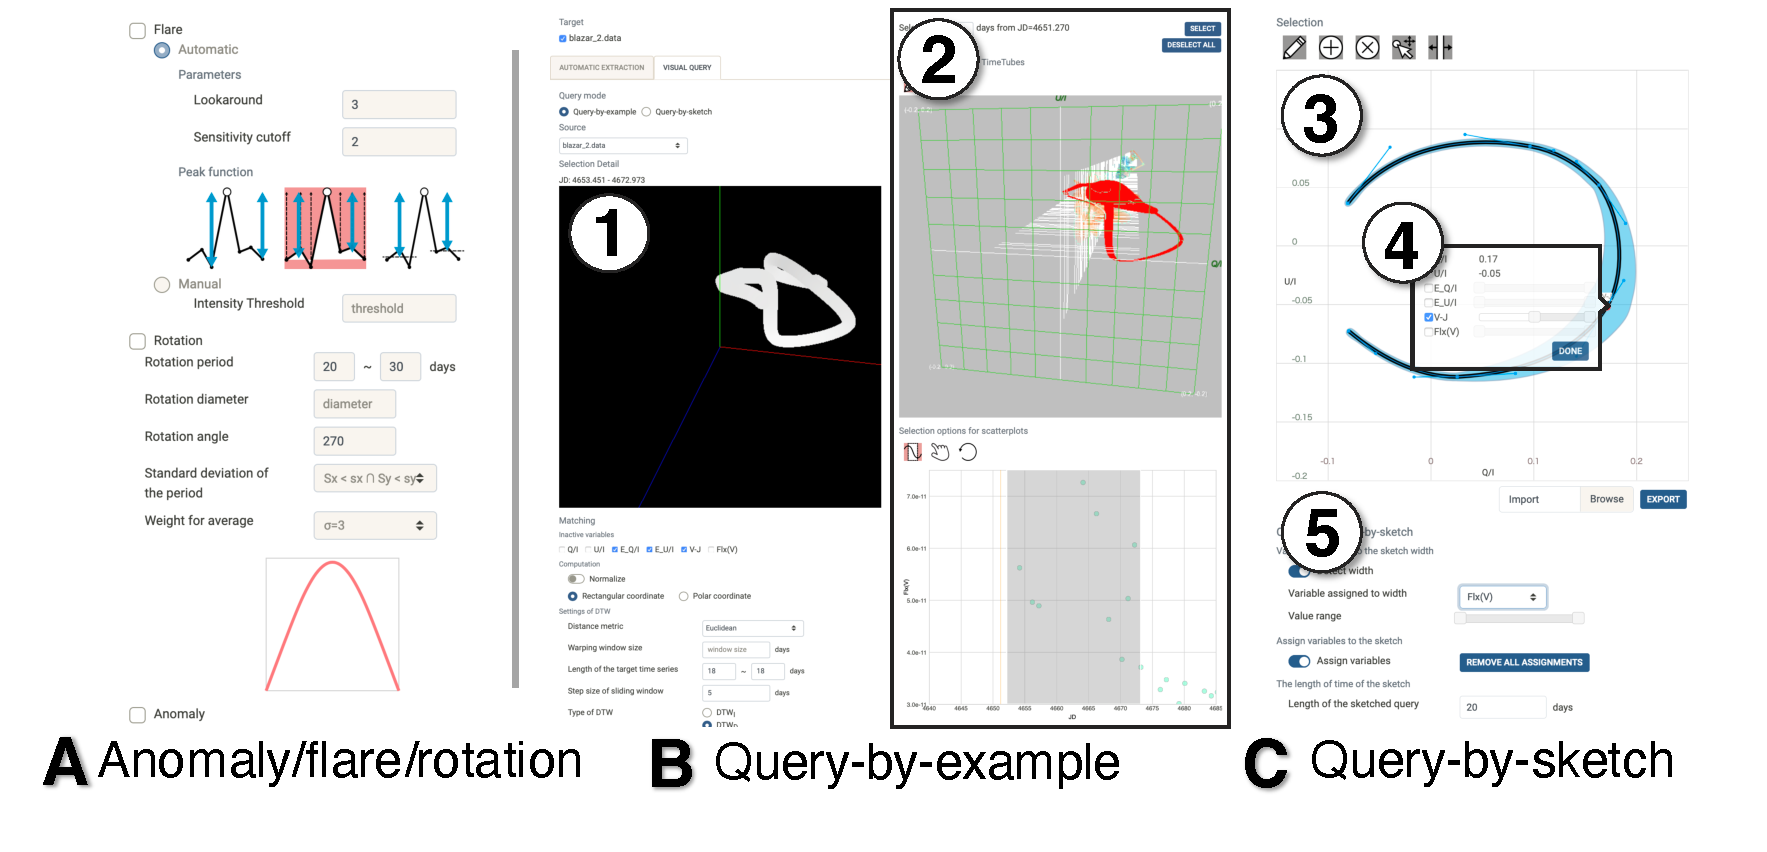
\includegraphics[width=.99\linewidth]{vgtc_journal_latex/figures/QuerySpecificationPanel.pdf}
    %     \end{center}
    %     \begin{minipage}{\columnwidth}
    %     \caption{User interface for feature extraction and dynamic visual queries. Automatic feature extraction is illustrated in (A).
    %     , one with query-by-example in (B), and one with query-by-sketch in (C). 
    %     To query-by-example (B), users select a time interval in the TimeTubes or scatterplots views (2) and can check the selected time interval in a 3D tube view and further fine-tune query parameters (1). %The current query is shown as 3D tube an can be fine-tuned  (2). 
    %     To query-by sketch (C), users draw a SOI (1) and can adjust variables at each control point of the hand-drawn sketch (2) or adjust general sketch pad settings (3).}
    %     \label{fig:querySpecificationPanel}
    %     \end{minipage}
    % \end{minipage}
\end{figure}
\begin{figure}[t]
    \begin{minipage}{\columnwidth}
        \begin{center}
            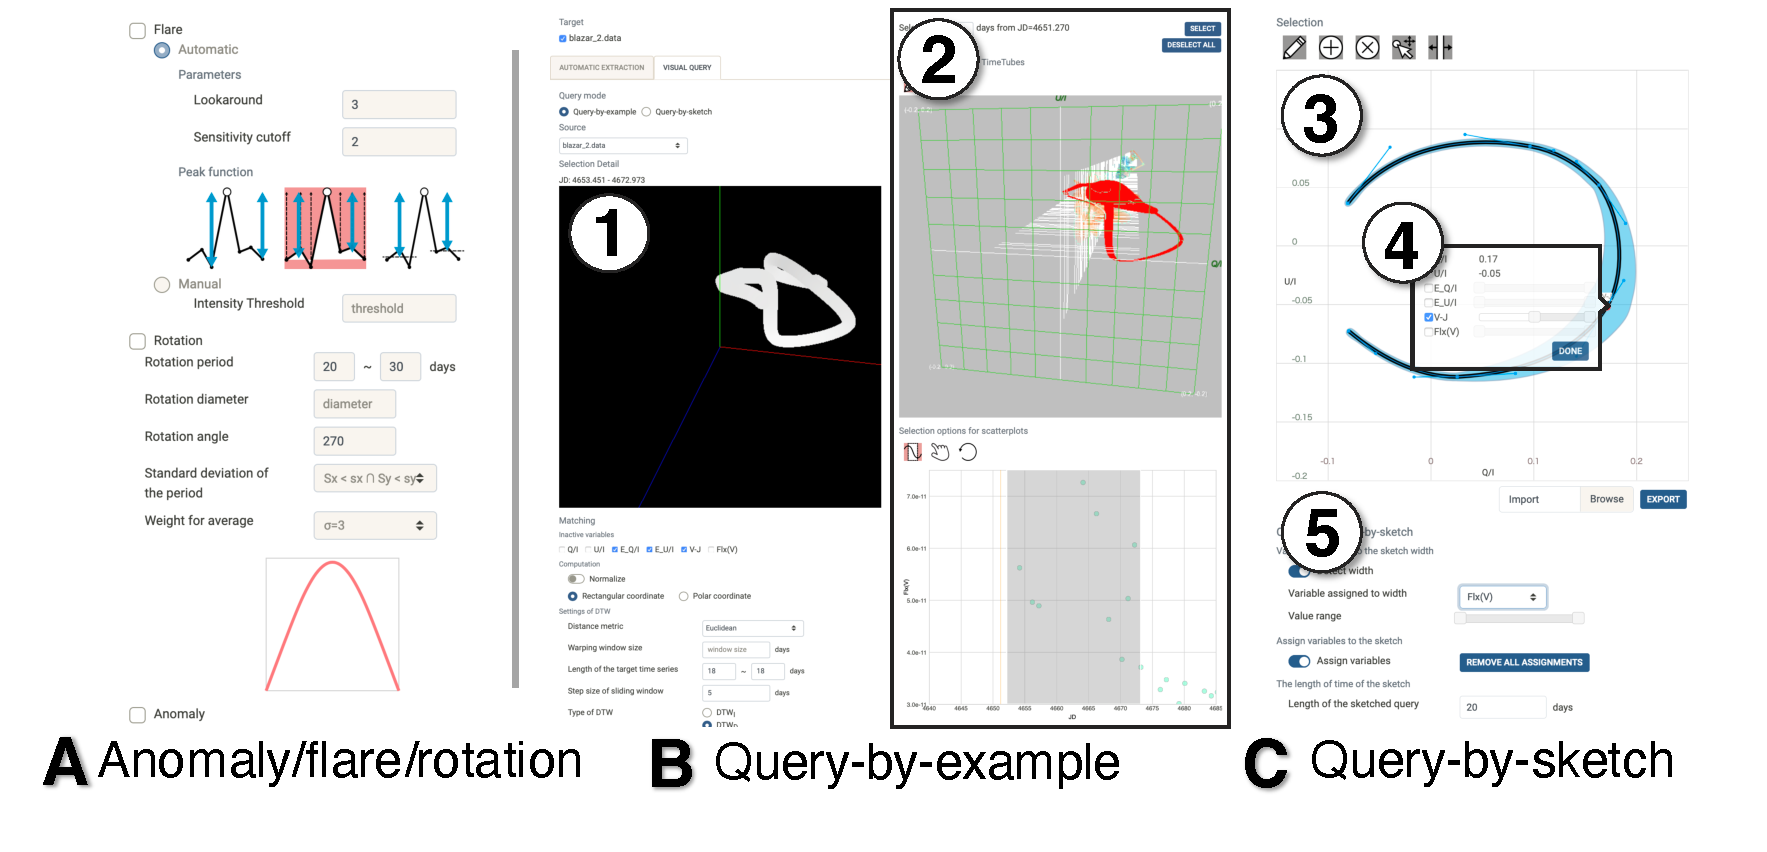
\includegraphics[width=.99\linewidth]{vgtc_journal_latex/figures/QuerySpecificationPanel.pdf}
        \end{center}
        \begin{minipage}{\columnwidth}
        \caption{Query specification panels for feature and pattern detection methods. (A) Automatic feature extraction; (B) Query-by-example. Users can check the selected time interval in a 3D tube view and further fine-tune query parameters (1) after they select a time interval in the TimeTubes or scatterplots views (2);
        % users select a time interval in the TimeTubes or scatterplots views (2) and can check the selected time interval in a 3D tube view and further fine-tune query parameters (1). %The current query is shown as 3D tube an can be fine-tuned  (2). 
         and (C) Query-by-sketch. Users draw a SOI (3) and can assign filtering constraints at each control point of the hand-drawn sketch (4) or adjust general sketch pad settings (5).}
        \label{fig:querySpecificationPanel}
        \end{minipage}
    \end{minipage}
\end{figure}
\begin{figure}[t]
    \centering
    \vspace{3mm}
    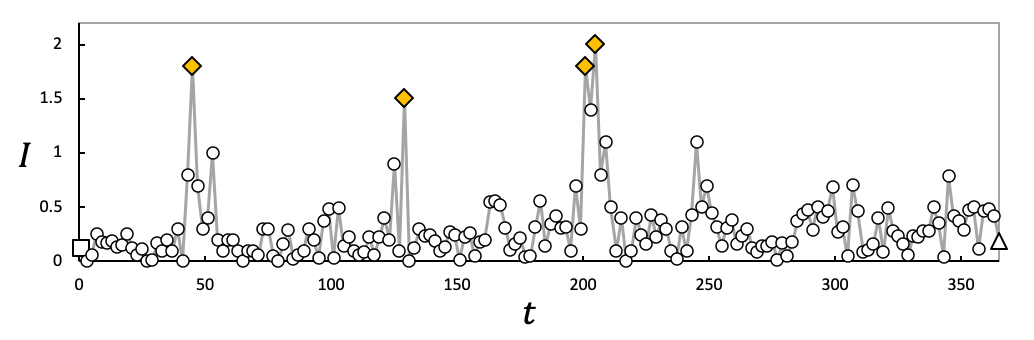
\includegraphics[width=.8\linewidth]{vgtc_journal_latex/figures/synthesisDataLightCurveLabel_revised.png}\\
    \footnotesize{\sf (a) Light curve plot. The orange diamonds indicate peaks in the data.}\\
    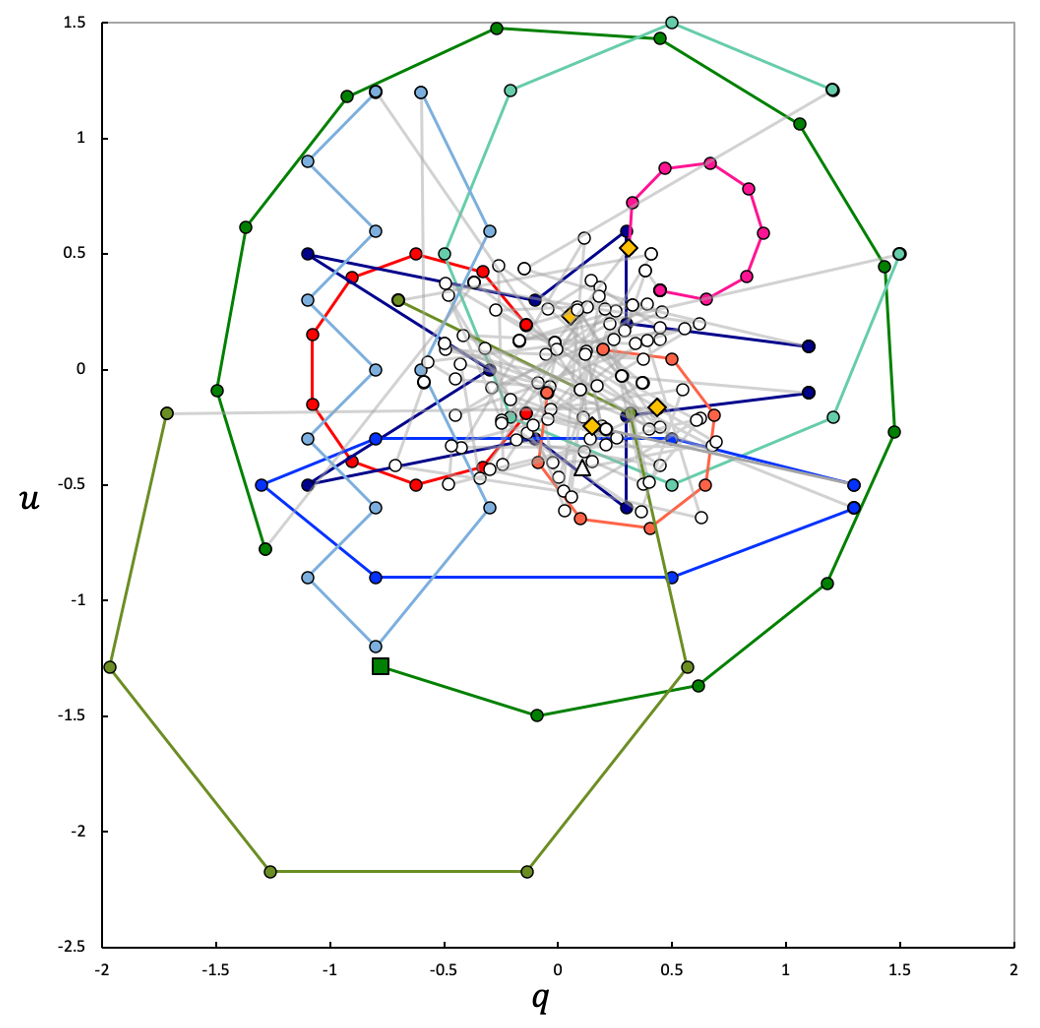
\includegraphics[width=.83\linewidth]{vgtc_journal_latex/figures/synthesisDataStokesLabel_revised.png}\\
    \footnotesize{\sf (b) Stokes plane plot. The orange diamonds indicate the peaks in (a).}
    \caption{Conventional light curve plots and the Stokes plane for our synthetic dataset. The data has three small circular patterns (red), three big rotations (green), and three narrow/rough-edged patterns (blue) within 365 days. Data starts from a square mark and ends at a triangular mark.}
    \label{fig:synthesisData}
\end{figure}
% \begin{figure}[t]
%     \centering
%     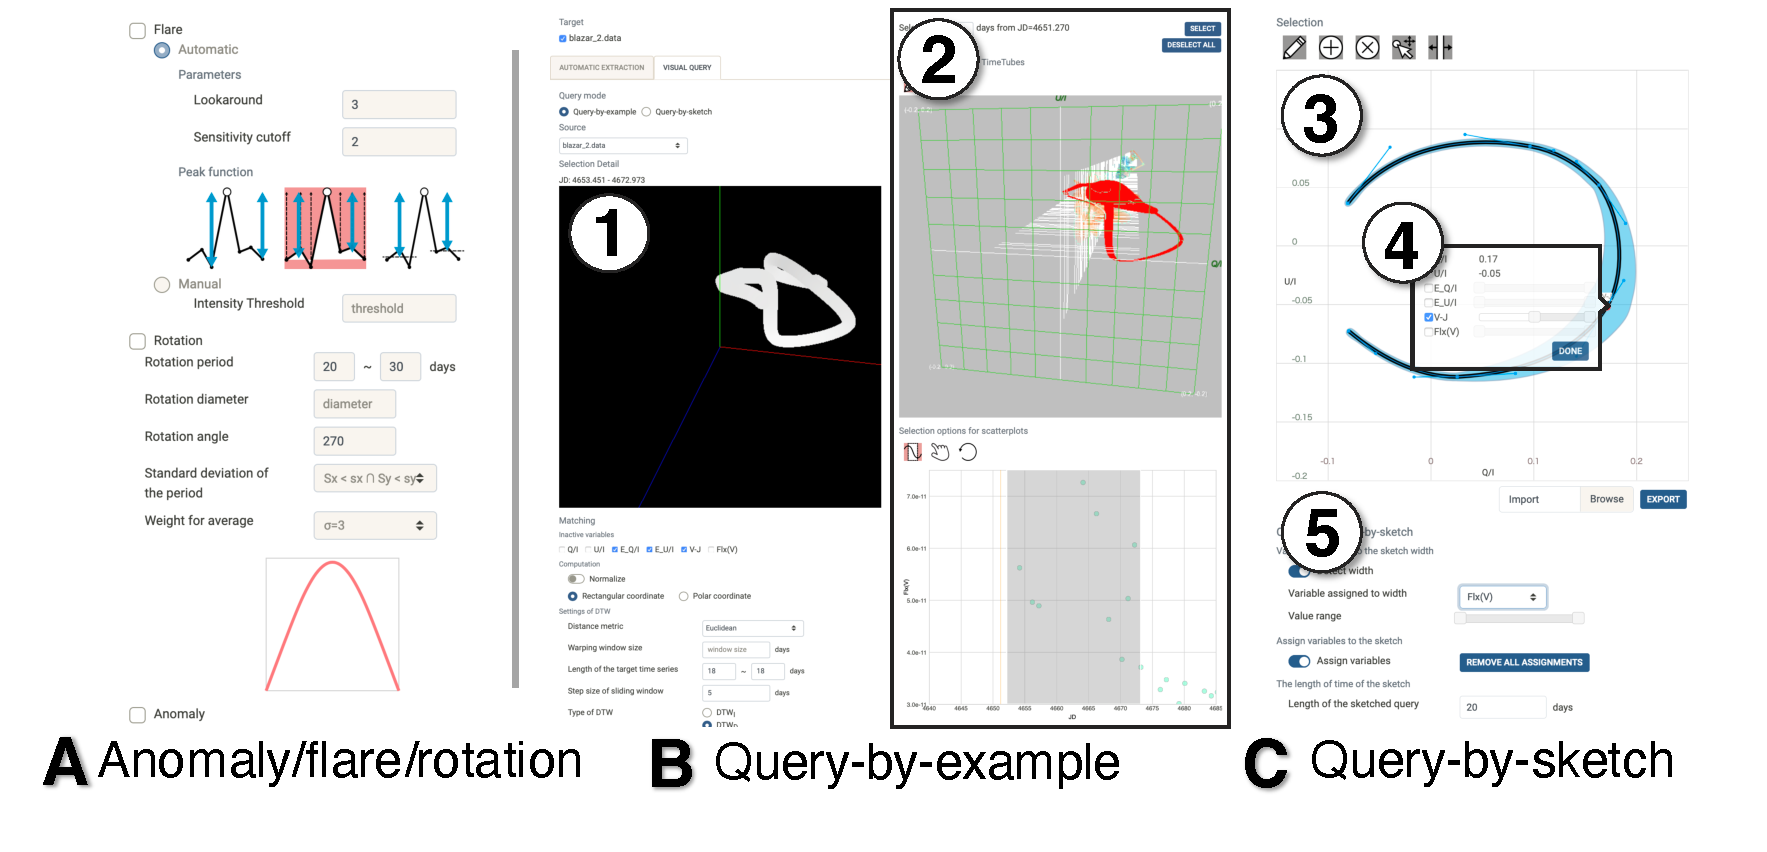
\includegraphics[width=.99\linewidth]{vgtc_journal_latex/figures/QuerySpecificationPanel.pdf}
%     \caption{Caption}
%     \label{fig:my_label2}
% \end{figure}
\section{Automatic Feature Extraction}\label{sec:automaticExtraction}
Astronomers pay careful attention to unusual behaviors of blazars, such as flare and rotation.
As a first step to identify flares and rotations (\textbf{G2}),
we have implemented automatic feature extraction for the discovery and analysis of dynamic time variations (\textbf{T3}).
TimeTubesX automatically extracts three types of features: anomalies (Section~\ref{sec:anomalyDetection}), flares (Section~\ref{sec:flareDetection}), and rotations (Section~\ref{sec:rotationDetection}).
% As the first step for quickly finding such behaviors, 
% TimeTubesX supports automatic feature extraction for three types of features: anomalies, flares, and rotations. %; flare detection; and rotation detection. 
We have significantly improved the detection algorithms for flares and rotations compared with the ones in our previous work~\cite{Sawada2018} 
to identify flares more flexibly and detect rotations more accurately.
% The automatic feature extraction allows users to quickly identify candidate time intervals for known blazar behaviors.
%It supports the users' efficient analysis through quick access to candidates for observable behaviors.
Fig.~\ref{fig:querySpecificationPanel} (A) shows the automatic feature extraction panel, %query specification panel
where users can select specific patterns and parameters for automatic feature extraction.
%the users select what to detect and then input parameters for matching.
%3D tube views for the time intervals including an anomaly, flare, and rotation are provided in
The node (A) in Fig.~\ref{fig:framework} shows example TimeTubes views for an anomaly, flare, and rotation.
% all three supported blazar patterns (i.e., anomaly, flare, rotation).

\subsection{Anomaly Detection}\label{sec:anomalyDetection}
It is challenging for astronomers to manually identify time variations across multiple variables. 
We define data samples with drastic temporal changes in polarization, intensity, and color as \textit{anomalies}.
Tracking anomalies can result in identifying unusual time variations or presages of well-known behaviors, such as flares or rotations,
because observable blazar behaviors show a tendency to include these drastic variations.

The anomaly degree was defined in our previous work~\cite{Sawada2018} as the product of the change amount in polarization, intensity, and color per day:
\begin{equation*}
\begin{split}
  \int_t^{t + 1}\left|\frac{dPolar(t)}{dt}\right|\cdot\left|\frac{dI(t)}{dt}\right|\cdot\left|\frac{dC(t)}{dt}\right|dt,
  \label{eq:anomaly}
\end{split}
\end{equation*}
where $Polar(t)$ means the position of a data sample on the Stokes plane at time $t$, and $I(t)$ and $C(t)$ stand for intensity and color, respectively. 
%In the anomaly detection, observation errors have not been taken into account for the sake of simplicity.

\textsf{Experimental results.\ } Applying the anomaly detection to our synthetic data, 
data samples around extreme peaks (the orange diamonds in Fig.~\ref{fig:synthesisData}~(a)) and parts of dynamic rotations (the green plots in (b)) were highly ranked.


\subsection{Flare Detection}\label{sec:flareDetection}
Flares are defined as extreme peaks of brightness (i.e., emitted light intensity). 
Astronomers regard flares as one of the most important observed behaviors of blazars.
However, since there is no specific threshold value of $I$ to define a flare, 
they need to analyze the local temporal profile of $I$ to identify flares.
We have updated the flare detection methods used in our previous work~\cite{Sawada2018}
to detect relatively small local flares as well as globally large flares.
To that end, we utilize peak detection methods for time-series data~\cite{Palshikar2009} to extract flare candidates. 
Flare detection comprises the following two steps:
\begin{enumerate}[nosep, label=\textsl{Step \arabic*}:, ref=\textsl{Step \arabic*}, align=parleft, leftmargin=*]
    \item \textsl{Compute the spikiness score $S$ for each data sample}; \label{algo:flareSpikiness}
    \item \textsl{Filter out data samples with a globally small $S$}. \label{algo:flareFilter}
    % whose $S$ is small in a global context}. \label{algo:flareFilter}
\end{enumerate}
TimeTubesX uses Equation~\ref{equ:S2} to compute the spikiness score $S$ for \ref{algo:flareSpikiness};
we tested multiple equations for $S$ and empirically found that the following one produces the best results:
\begin{eqnarray}
    % S_1 &=& \frac{\underset{1 \leq k \leq K}{\max}\{x_i - x_{i - k}\} + \underset{1 \leq k \leq K}{\max}\{x_i - x_{i + k}\}}{2}\label{equ:S1}\\
    S &=& \frac{\frac{\sum_{k=1}^{K}(x_i - x_{i - k})}{K} + \frac{\sum_{k=1}^{K}(x_i - x_{i + k})}{K}}{2}\label{equ:S2},
    % S_3 &=& \frac{\left(x_i - \frac{\sum_{k=1}^{K}{x_{i - k}}}{K}\right) + \left(x_i - \frac{\sum_{k=1}^{K}{x_{i + k}}}{K}\right)}{2}\label{equ:S3}
\end{eqnarray}
where $x_i$ denotes a data sample indexed as $i$ and $K$ denotes the number of neighbors that should be examined.
% \autoref{equ:S1} computes the average of the maximum differences between a focused data sample $x_i$ and $K$ left and right neighbors of $x_i$.
Equation~\ref{equ:S2} provides the average values of the averages of distances between $x_i$ and $K$ left neighbors and those between $x_i$ and $K$ right neighbors.
% \autoref{equ:S3} computes the average of distances between $x_i$ and the mean of $K$ left and right neighbors. 
% Because flares tend to have small peaks before or after the flare, 
\ref{algo:flareFilter} retains only data samples that satisfy $S - \bar{S} > h \times \sigma_{S}$, 
where $\bar{S}$ and $\sigma_{S}$ denote the mean and standard deviation of all computed $S$ values for the dataset, respectively, 
and $h$ is a user-specified sensitivity threshold. 
The original algorithm~\cite{Palshikar2009} merges peaks that are close together into one, 
but we did not adopt this strategy
because astronomers are equally interested in small, individual flares and large, aggregated flares.
% also interested in small individual flares rather than just big aggregated flares.


\begin{figure}[tb]
    \centering
    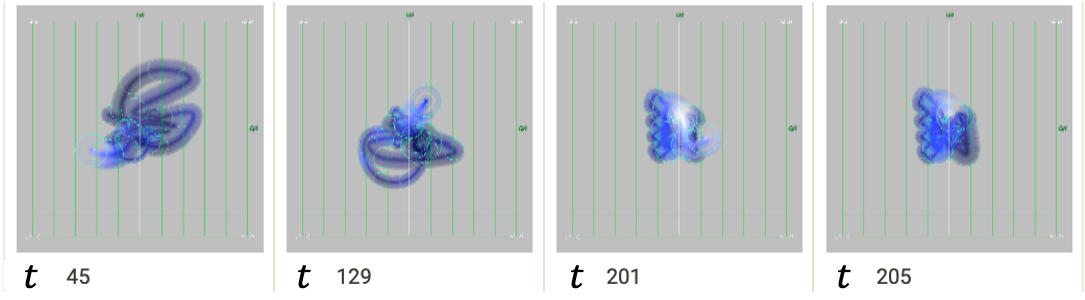
\includegraphics[width=.85\linewidth]{vgtc_journal_latex/figures/flareDetectiondemodataResults.png}
    \caption{Flare detection results for our synthetic data. The results match the four red data samples in Fig.~\ref{fig:synthesisData}~(a).}
    \label{fig:flareDetection}
\end{figure}
\begin{figure}[tb]
    \centering
    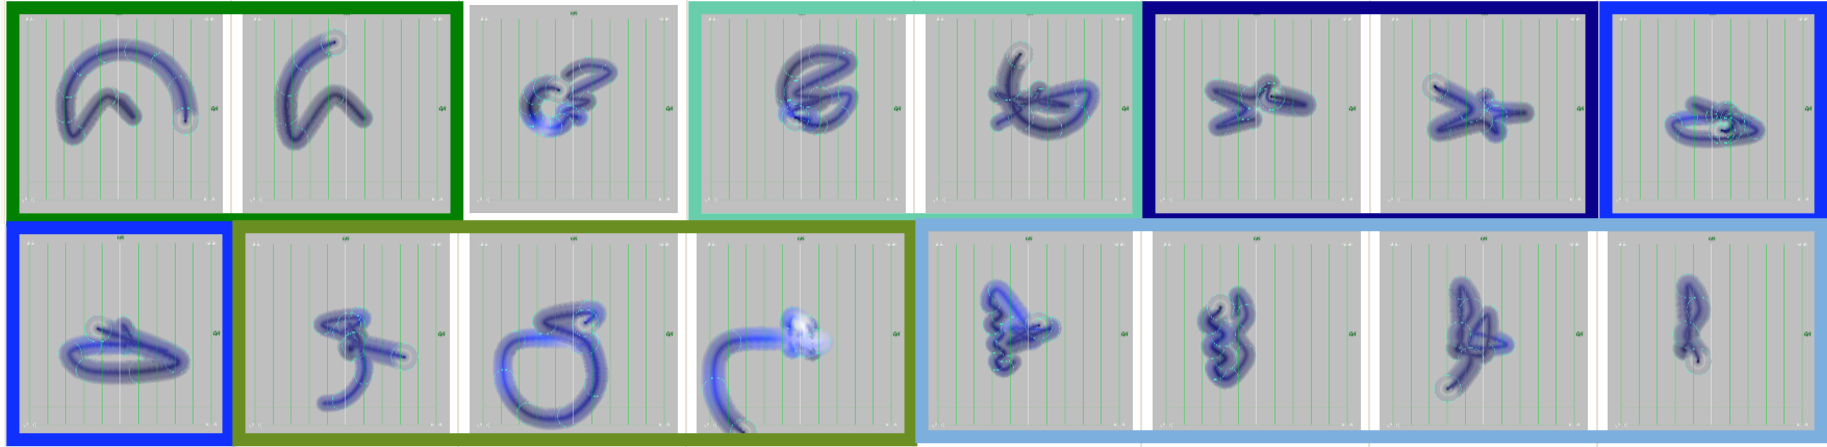
\includegraphics[width=\linewidth]{vgtc_journal_latex/figures/rotationDetectiondemodataResultsOR.png}\\
    \footnotesize{\sf(a) Previous rotation detection method~\cite{Fujishiro2018}.}\\
    \vspace{5px}
    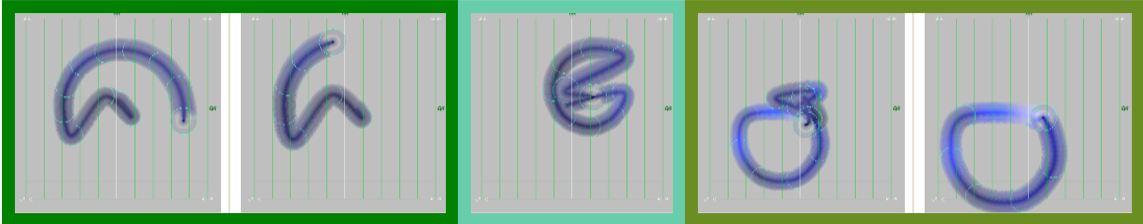
\includegraphics[width=.8\linewidth]{vgtc_journal_latex/figures/rotationDetectiondemodataResults.png}\\
    \footnotesize{\sf(b) Our improved method.}
    \caption{Rotation detection results for our synthetic dataset in Fig.~\ref{fig:synthesisData}. 
        The outline color corresponds to the color in Fig.~\ref{fig:synthesisData}~(b).
        Our previous method detected narrow/rough-edged patterns and noise (blue), 
        whereas our improved method detected only large rotations (green).}
    \label{fig:rotationResults}
\end{figure}

\textsf{Experimental results.\ } We applied the flare detection method to our synthetic data.
We set $K$ and $h$ to 3 and 1, respectively.
Fig.~\ref{fig:flareDetection} presents the flare detection results.
The four data samples were detected as flares,
which completely coincide with the deliberately generated peaks that are highlighted in orange in Fig.~\ref{fig:synthesisData}~(a).

\subsection{Rotation Detection}\label{sec:rotationDetection}
Polarization rotation is another important observed behavior of blazars. 
Astronomers do not yet agree on whether rotation is an actual feature or just a result of random variations of polarization.
To validate their hypotheses, they scrutinize correlations between polarization and other properties at the time interval.
They typically have been analyzing the time variation of $PA$ to identify rotations~\cite{Ikejiri2011, Uemura2017},
but the rotation center will not be located at the origin of the Stokes plane ($(q, u) = (0, 0)$) when there are multiple polarized components in the sky.
Thus, estimating a rotation only through $PA$ may not allow astronomers to adequately understand its behavior.
Our rotation detection is capable of addressing any rotations regardless of the position of the rotation center.

We use a sliding window approach that allows users to manually define the length of the time interval for the sliding window. Based on feedback from astronomers~\cite{Sasada2012}, we set the default window size to be between three and four weeks.
%Using a sliding window approach, the rotation detection picks up a time interval from a long-term dataset. 
%Users can freely determine the time interval length, 
%whose default setting we empirically decided from three weeks to a month according to the prior report by the astronomers~\cite{Sasada2012}.

The computation of the rotation angle is divided into the following seven steps:
\begin{enumerate}[nosep, label=\textsl{Step \arabic*}:, ref=\textsl{Step \arabic*}, align=parleft, leftmargin=*]
    \item \textsl{Compute the weighted means ($\overline{q}, \overline{u}$) of $q$ and $u$ at the time interval};\label{algo:rotationMean}
    \item \textsl{Compute the standard deviations ($\sigma_{q}, \sigma_{u}$) of $q$ and $u$ at the time interval}; \label{algo:rotationStd}
    \item \textsl{Convert the rectangular coordinates ($q-u$ domain) to polar coordinates ($r - \theta$ domain) with its origin shifted to $(\overline{q}, \overline{u})$}; \label{algo:rotationPolar}
    \item \textsl{Filter out time intervals whose $\sigma_{q}$ or $\sigma_{u}$ is smaller than the standard deviations of the entire dataset}; \label{algo:rotationFilter}
    \item \textsl{Compute the difference ($\theta_{\rm diff}$) of the $\theta$'s of two consecutive data samples}; \label{algo:rotationDiff}
    \item \textsl{Sum $\theta_{\rm diff}$'s to yield $\theta_{\rm sum}$}; \label{algo:rotationSum}
    \item \textsl{Check whether $\theta_{\rm sum}$ is larger than the user-specified threshold for the total rotation angle}. \label{algo:rotationThreshold}
\end{enumerate}
We regard $\overline{q}$ and $\overline{u}$ as a rotation center. 
To avoid misleading effects of outliers and unexpected values at the edges of a time interval,
% our detection method uses weighted mean values at \ref{algo:rotationMean}. 
smaller weights are assigned to both ends of the time interval according to a Gaussian distribution at \ref{algo:rotationMean}.
% while heavier weights are assigned to its center according to a Gaussian distribution. %as the rotation center of the focused time interval at \ref{algo:rotationMean}.
Note that users are allowed to adjust these weight ratios.
%
To avoid misclassifying time intervals with large $q$ or $u$ variance and unlike rotations as rotation candidates,
we have improved upon our previous rotation detection method~\cite{Sawada2018} on the basis of feedback from two astronomers at Hiroshima University~\cite{Huang2019}.
%
%In our previous short paper~\cite{Sawada2018}, 
%we filter out only time intervals \textbf{both} of whose $\sigma_{q}$ \textbf{and} $\sigma_{u}$ are smaller than the standard deviation of the entire dataset. 
%However, several astronomers in Hiroshima University reported that the previous rotation detection sometimes detects time intervals with large $q$ or $u$ variance and unlike rotations~\cite{Huang2019}.
%To address this problem, the current 
%
To detect only large rotations, 
our new method is able to filter out time intervals in which \textbf{either} $\sigma_{q}$ \textbf{or} $ \sigma_{u}$ is smaller than the standard deviation of the entire dataset. % avoid small or narrow patterns.
%The up-to-date version provides 
Note that this and other provided filtering constraints also allow for discovery of small or narrow rotations, such as the red and blue patterns in Fig.~\ref{fig:synthesisData}~(b).
% Additionally, we provide multiple filters on standard deviations of the time intervals as well as the previous filter, to find out small rotations.
%
At \ref{algo:rotationDiff}, we cannot compute $\theta_{\rm diff}$ simply by subtracting the $\theta$'s of consecutive observations 
due to the range constraint on $\theta_{\rm diff}$ (i.e., $\theta_{\rm diff} \in [0, 2\pi]$). 
For example, when two successive data samples are located in the first and fourth quadrant of the Stokes plane, 
we need to consider whether to take the clockwise or counterclockwise direction as $\theta_{\rm diff}$. 
We determine the rotation direction 
by checking increasing/decreasing tendency in $\theta$'s with exponential smoothing~\cite{Brown1956}.
% by comparing the predictive values for $\theta$'s, which we can derive by exponential smoothing~\cite{Brown1956}.
% which is a forecasting method
% for time-series datasets to predict a subsequent value based on previous values. 
% that produces a weighted average of past observations. 
It forecasts the next value according to past observations by assigning larger weights to more recent observations.
In this way, it addresses the uncertainty about the rotation direction and make results more feasible (\textbf{T1}).
% If the predictive value derived by exponential smoothing increases, 
% the rotation direction tends to be counterclockwise;
% otherwise, it is clockwise.
We estimate the variation trend of $\theta$ and
then define the angle in the predicted rotation direction as $\theta_{\rm diff}$.
Users can set an arbitrary angle as a threshold parameter at \ref{algo:rotationThreshold}.

\textsf{Experimental results.\ } To compare our novel algorithm with the previous rotation detection algorithm~\cite{Sawada2018}, we applied both to our synthetic data.
As the results in Fig.~\ref{fig:rotationResults}~(a) show, 
the previous algorithm detected not only large rotations (green patterns in Fig.~\ref{fig:synthesisData}~(b)) but also narrow or rough-edged patterns (blue).
The improved algorithm more accurately detected only time intervals in which the polarization values dynamically rotate (green), as shown in Fig.~\ref{fig:rotationResults}~(b).
% Note that users can also detect small or narrow rotations such as red or blue patterns in \autoref{fig:synthesisData}~(b) 
% by changing filtering constraints on $\sigma_{q}$ and/or $ \sigma_{u}$.
% The previous method detects time intervals which have large variances in the $x$ or $y$ axis direction as rotation candidates. 
% Some of them seem to just behave messily and not rotate. 
% We apply the improved method to the same synthetic data. 
% The detection results are displayed in Fig.~\ref{fig:rotationResults}~(b). 
% In comparison with (a), it seems that time intervals with messy variations are omitted from the results. 
% With the improvements, the up-to-date rotation detection can find out time intervals where the polarization values dynamically rotate.

% \subsection{Anomaly and flare with a rotation}
% Some astronomers reported that rotations tend to co-occur with flares~\cite{Ikejiri2011}.
% The automatic feature extraction can find out a rotation including anomalies or flares inside its time interval 
% by combining the anomaly detection in \autoref{sec:anomalyDetection} or the flare detection in \autoref{sec:flareDetection} with rotation detection in \autoref{sec:rotationDetection}.



% We improve the detection algorithms for the initial version of the automatic feature extraction in \cite{Sawada2018}. 

% The following parts dig into each of the options.
% The automatic feature extraction is particularly important for task \textbf{T3}.


% TODO: Update figures!
% \begin{figure}[tb]
%     \centering
%     \begin{minipage}{.44\linewidth}
%         \centering
%         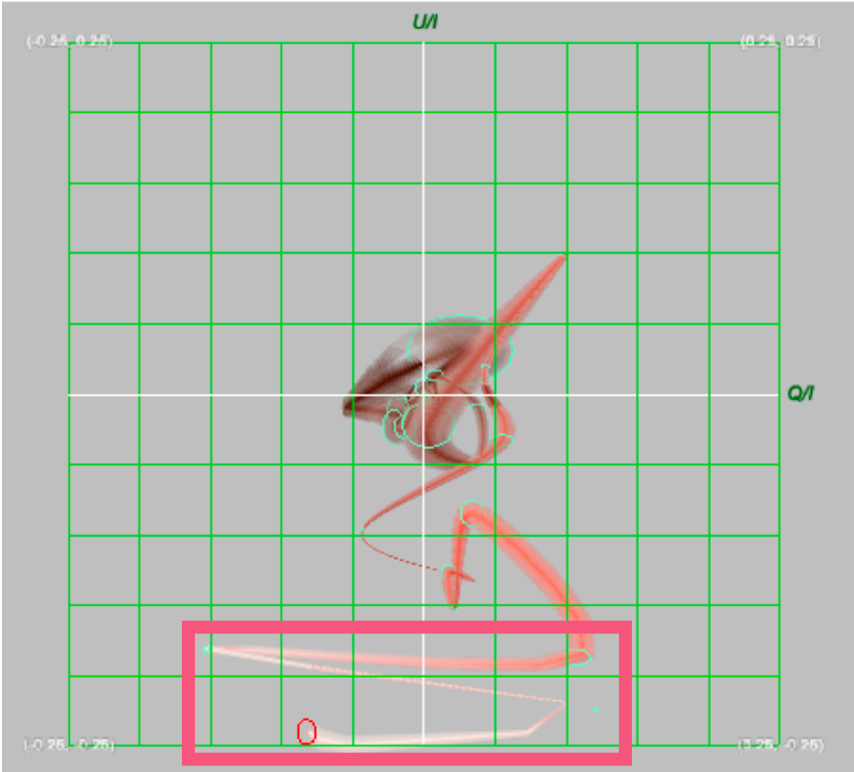
\includegraphics[width=0.99\linewidth]{vgtc_journal_latex/figures/flareExampleTimeTubes.png}
%     \end{minipage}
%     \begin{minipage}{.55\linewidth}
%         \centering
%         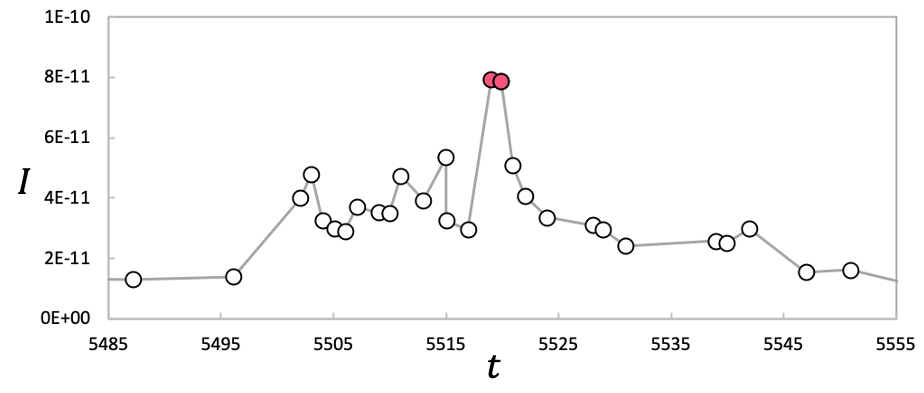
\includegraphics[width=.99\linewidth]{vgtc_journal_latex/figures/flareExampleSP.png}
%     \end{minipage}
%     \begin{minipage}{.44\linewidth}
%         \centering
%         \textsf{\footnotesize (a)~TimeTubes view.}
%     \end{minipage}
%     \begin{minipage}{.55\linewidth}
%         \centering
%         \textsf{\footnotesize (b)~Light curve.}
%     \end{minipage}
%     \caption{Flare of a blazar \textbf{3C 454.3} at $t=5{,}518.98$. The flare part is highlight in red in both of TimeTubes and scatterplots views.}
%     \label{fig:flareExample}
% \end{figure}

% In \autoref{fig:flareExample}, 
% a flare occurrence in the blazar, named \textbf{3C 454.3}, around $t = 5{,}518.98$ is visualized by TimeTubes~(a) and light curve~(b).
% In such a short period, the intensity drastically increases and decreases. 
% In (a), the color of the tube looks much brighter in the part enclosed by a red rectangle than the other parts.
% Data samples enclosed by the red rectangle in (a) coincide with red plots in (b).

% though the time intervals with sharp peaks are considered to be flares.

% To test the flare detection, we used a synthetic data in \autoref{fig:synthesisData}.
% In (a), a square plot means the first data sample, while a triangular the last data sample.


% \begin{figure}
%     \begin{minipage}{0.49\linewidth}
%         \centering
%         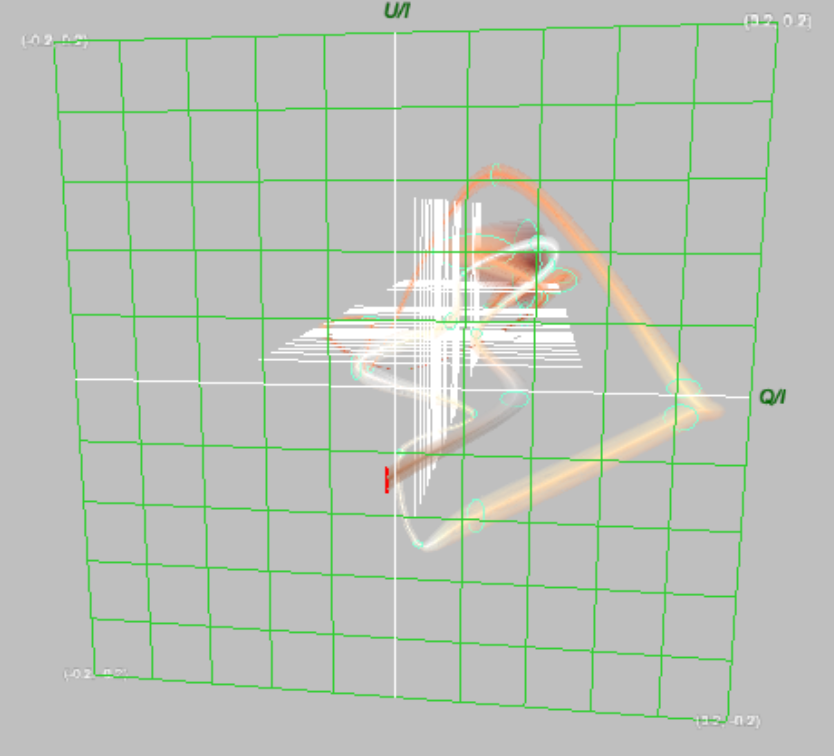
\includegraphics[width=.95\linewidth]{vgtc_journal_latex/figures/TimeTubes_rotation.png}
%         \footnotesize{\sf (a)~TimeTubes view.}
%     \end{minipage}
%     \begin{minipage}{0.49\linewidth}
%         \centering
%         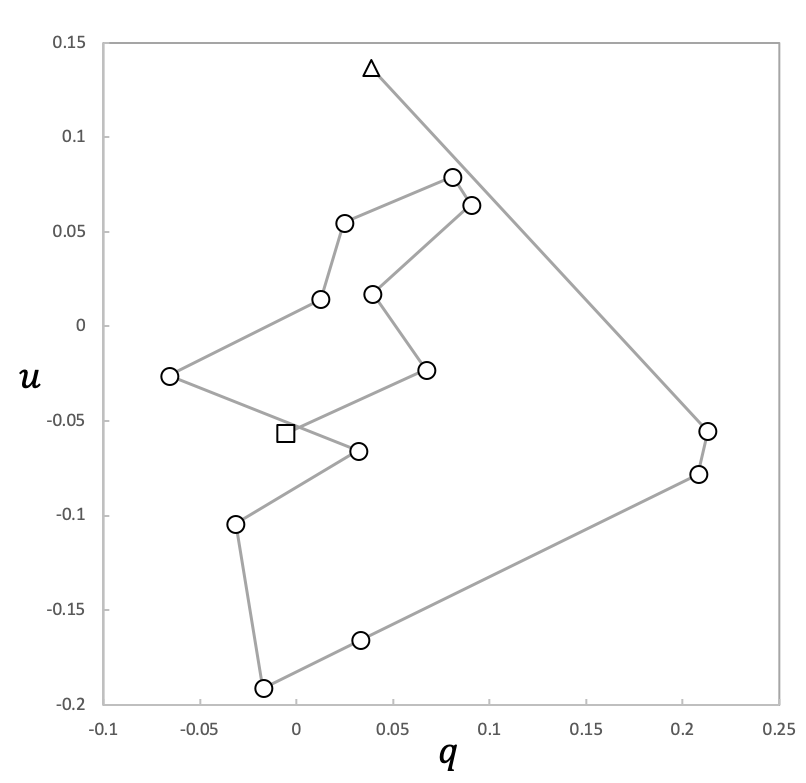
\includegraphics[width=.95\linewidth]{vgtc_journal_latex/figures/ScatterPlot_rotation.png}
%         \footnotesize{\sf (b)~Scatterplots view.}
%     \end{minipage}
%     \caption{Rotation of \textbf{3C 454.3} in the time interval $[5{,}156, 5{,}186]$. TimeTubes view provides an oblique view to show 3D structure of the tube. We connect data samples in chronological order, where the period starts from a square plot and end at a triangular plot.}
%     \label{fig:rotationExample}
% \end{figure}

% The dynamic rotation on the Stokes plane can be characterized with variation of $PA$ in \autoref{eqn:PA}.

% It is still controversial among the astronomers. 

% \autoref{fig:rotationExample} shows TimeTubes view~(a) and scatterplots view~(b) of the time interval $[5{,}156, 5{,}186]$ for \textbf{3C 454.3} including a behavior regarded as a rotation. 
% \autoref{fig:rotationExample}~(b) shows scatterplots for the Stokes plane,
% where the plots are connected with a polygonal line in chronological order,
% where the rotating behavior starts from a square plot and ends at a triangular plot.
% The polarization values do not necessarily rotate around the origin of the Stokes plane, 
% that is $(q, u) = (0, 0)$, as shown in \autoref{fig:rotationExample}.
% due to the inconsistent position of the rotation center.


% We recommend users to use the weighted mean instead of the arithmetic mean 
% because outliers or unexpected values at the edges of the time interval can directly affect the arithmetic mean.


% whereas the previous version filters out only time intervals \textit{both} of whose standard deviations of $\sigma_{Q/I}$ and $ \sigma_{U/I}$ larger than them. %the global standard deviations.
% With this improvements, the up-to-date version detects only time intervals where the polarization values dynamically rotate.

% \begin{figure}[tb]
%     \centering
%     \includegraphics[width=.99\linewidth]{images/RotationDetectionOR.png}\\
%     \footnotesize{\sf (a)~Previous method.}\\
%     \includegraphics[width=.99\linewidth]{images/RotationDetectionAND.png}\\
%     \footnotesize{\sf (b)~Improved method.}
%     \caption{The rotation detection results for a randomly generated synthetic data. 
%         (a)~Time intervals with large variance are also detected as rotations.
%         (b)~Time intervals which vary largely in both of $x$ and $y$ axes directions are detected.
%     }
%     \label{fig:rotationResults}
% \end{figure}
\section{Dynamic Visual Querying}\label{sec:visualQuery}
To facilitate astronomers' easy discovery of time intervals similar to a ROI/SOI (\textbf{G3}) or those validating specific hypotheses (\textbf{G4}), 
TimeTubesX provides two different user-initiative visual query interfaces: query-by-example (QBE) and query-by-sketch (QBS).
Both are designed to help users identify interesting similar patterns (\textbf{T4}), and our matching algorithm allows for a fuzzy search (\textbf{T5}).
% those more subtle than the well-known patterns described in \autoref{sec:automaticExtraction}.

\subsection{Query-by-Example}\label{sec:QBE}
% background and overview
While the TimeTubes view helps users analyze time variation patterns,
it still remains challenging for users to build queries for multi-dimensional, time-dependent data.
Our QBE interface allows users to specify an interesting behavior as a ROI with simple interactions through the TimeTubes or scatterplots views.
Users can not only pick a part of time-series data as an input for a query but also flexibly select specific variables that should be used in the query to reflect their intentions. 
This allows users to easily and intuitively search long-term datasets for interesting patterns with minimal required user inputs.

Fig.~\ref{fig:querySpecificationPanel} (B) shows our QBE interface.
% First, users specify the time interval by either clicking on the corresponding slice in the 3D Timetubes view, or by defining a region in the scatterplot view (see \autoref{fig:querySpecificationPanel} (B)(1)).
To facilitate visual verification by users, a time interval selected through the TimeTubes or scatterplots views in (2, red highlight) is automatically extracted and displayed in the query panel (1).
% The selected time interval is highlighted in red in both views.
% Our system automatically extracts the selected time interval and displays it in the query panel (2) to facilitate visual verification by users.
After selecting the initial time interval, users can then fine-tune and adjust their query by selecting the variables that should be queried on. 
This is crucial for effective support of queries on multi-dimensional data.
Based on the selected variables, 
our system interactively updates the appearance of the 3D tube for the selected time interval in (1), visually encoding only currently selected variables.
For example, when users remove the variable $C$ from the query, the tube loses color variation and becomes a gray tube, as shown in (1).
% % high-level overview
% Our QBE interface was designed for time-dependent multi-dimensional data. 
% Users first pick the part of the dataset that should serve as input for a query. In a second step, however, they are also able to select the specific variables and the exact time span that should be used in the query, which is dynamically updated in the query panel (see \autoref{fig:querySpecificationPanel} (B)).
% This makes it easier for users to fine-tune and adjust queries for highly complex datasets.
% %
% %\autoref{fig:querySpecificationPanel} (B) shows our QBE panel.
% % THIS IS JUST UI
% We allow users to select a ROI for their query directly in the TimeTubes or scatterplot views.
% First, users specify the time interval by either clicking on the corresponding slice in the 3D Timetubes view, or by defining a region in the scatterplot view (see \autoref{fig:querySpecificationPanel} (B)(1)).
% %a part of the 3D tube or setting a region on scatterplots view, as shown in part (1). 
% The selected time interval is highlighted in red in both views. % of TimeTubes and scatterplots.
% %
% % THIS IS MUCH MORE INTERESTING - highlight WHY you are doing this (multi-dim queries, visually define those, give immediate user feedback)
% Our system automatically extracts the selected time interval and displays it in the query panel (2) to facilitate visual verification by the user.
% %as another 3D tube for the users to easily validate what they selected in part (2).
% After selecting the initial time interval, users can then fine-tune their query by selecting the variables that should be included in the query. This is crucial to support queries on multi-dimensional data.
% Based on the selected variables, 
% our system interactively updates the appearance of the 3D tube for the selected time interval, to only visually encode the currently selected variables.
% For example, when the users removes $C$ from the query, the tube loses color variation and becomes a gray tube, as shown in part (2).
After defining the query, users can adjust main parameters (i.e., normalization and polar coordinates options) for our matching algorithm (see Section~\ref{sec:matchingAlgorithm}). 
%We explain the matching algorithm between the query and time intervals in \autoref{sec:matchingAlgorithm}.
%
% Both options enable a fuzzy pattern search.
% %The Normalization option and polar coordinates option realize fuzzy pattern search.
% The normalization option triggers that the system normalizes the query and time intervals into the range of $[0, 1]$.
% Subsequently, the pattern search places great significance on the \emph{shape} of the time variations whereas the actual length of the time interval will be ignored.
% With the polar coordinates option, 
% $q(t)$ and $u(t)$ are converted into polar coordinates ($r-\theta$ domain) before computing similarities.
% Subsequently, the pattern search will also extract patterns that rotating around the origin of the Stoke plane.

\begin{figure}[tb]
    \centering
    \begin{minipage}{0.24\linewidth}
        \centering
        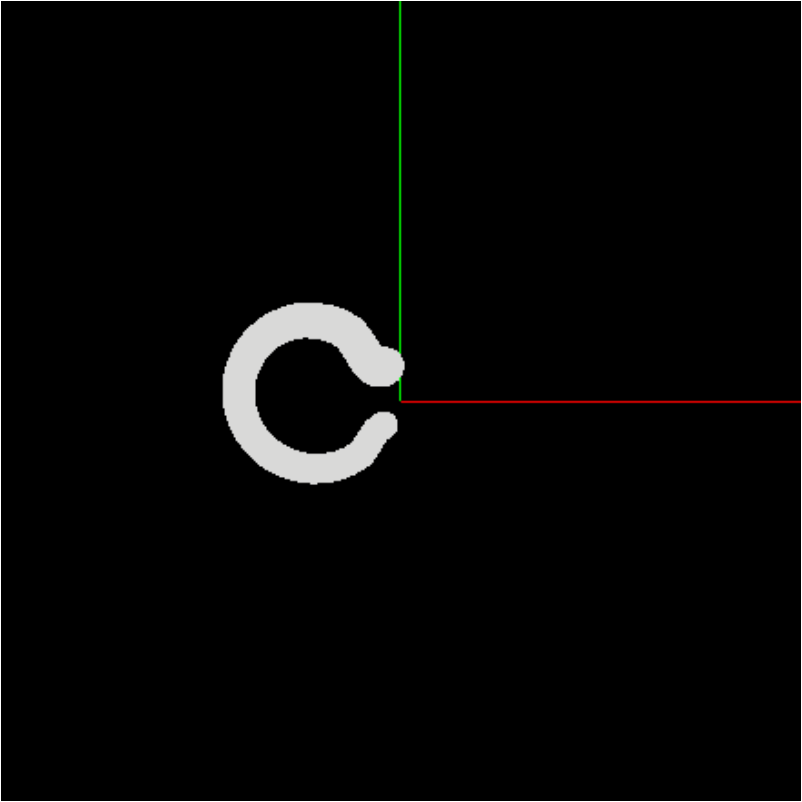
\includegraphics[width=.99\linewidth]{vgtc_journal_latex/figures/QBE.png}
        \footnotesize{\sf (a)~Query.}
    \end{minipage}
    \begin{minipage}{0.75\linewidth}
        \centering
        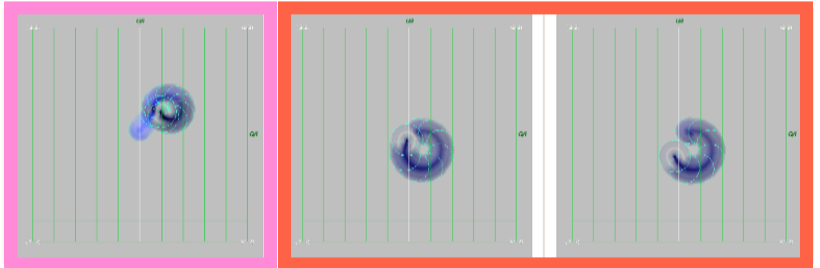
\includegraphics[width=.99\linewidth]{vgtc_journal_latex/figures/QBEdemodataResults.png}
        \footnotesize{\sf(b)~Results for the query in (a).}
    \end{minipage}
    \caption{QBE for our synthetic dataset in Fig.~\ref{fig:synthesisData}. 
        We pick the time interval with a small circular pattern (the leftmost red pattern in Fig.~\ref{fig:synthesisData}~(b)) for a query in (a). 
        Our method exactly extracted other time intervals with small circular patterns (the two red patterns from the right in Fig.~\ref{fig:synthesisData}~(b)).
        The outline color corresponds to the color in Fig.~\ref{fig:synthesisData}~(b).}
    \label{fig:QBEDemodata}
\end{figure}
\textsf{Experimental results.\ } We verified the effectiveness of our QBE method with our synthetic data.
The red circular patterns in Fig.~\ref{fig:synthesisData}~(b) have a similar shape but different time lengths, scales, or locations in the Stokes plane.
We used the leftmost red time interval in (b) as an input query, as shown in Fig.~\ref{fig:QBEDemodata}~(a).
We selected $q$ and $u$ as active variables and used the normalization and polar coordinates options to detect time intervals with different scales or different positions.
The length of the target time interval was set to 5 to 20 days.
% Due to the small size of the synthetic dataset, we set the sliding window step size to 2. 
We used $\rm{DTW}_{\rm D}$ as a distance function.
Note that we detail the options and parameters related to the matching process in Section~\ref{sec:matchingAlgorithm}.
Fig.~\ref{fig:QBEDemodata}~(b) shows the top three results of our QBE query.
The color of the rectangles corresponds to those used in Fig.~\ref{fig:synthesisData}~(b).
We were able to detect all time intervals with a similar shape in our synthetic dataset.
%The time intervals with a similar shape were definitely detected by the proposed QBE.
Note that the time interval specified for the query itself is omitted from the results.

\subsection{Query-by-Sketch}\label{sec:QBS}
% background and overview
TimeTubesX also allows users to query their data by manually drawing time variation patterns onto a 2D sketch interface.
Our QBS interface provides an intuitive and accessible way for users to specify patterns for complex multi-dimensional, semi-structured, time-dependent blazar datasets and to test their abstract hypotheses.
% To allow users to easily draw a pattern for multi-dimensional, semi-structured, time-dependent blazar datasets on a 2D sketch pad and test their abstract hypotheses of blazar behaviors, 
% we provide a novel QBS interface.
Rouxel et al.~\cite{Rouxel2014} state that an input trajectory by analog gestures are characterized by three dimensions: space, time, and force.
% To limit the complexity for users, our interface detects three input parameters: $x$ position, $y$ position, and either speed \emph{or} force.
To maintain the intuitiveness, 
we use space to determine the $x$ and $y$ positions of the stroke
and use either drawing speed or drawing pressure to define the stroke width 
so that users can describe time variations of multiple dimensions simultaneously.
Using the drawing speed option, the longer a cursor stays on a single point, the wider the curve at the point becomes.
To take into account other variables that are not described in sketching gestures, 
our QBS interface allows users to assign filtering constraints for each variable.
Thus, a sketch-based query for multi-dimensional, semi-structured, time-dependent data can be built with a single gesture
without sketching time variation patterns several times.

% ui and interactions
Fig.~\ref{fig:querySpecificationPanel} (C) shows the QBS query specification panel.
First, users define which variables are assigned to the $x$ and $y$ axes of the sketch pad and the stroke width (see panel (5)).
Second, they sketch a time variation pattern on a 2D sketch pad UI (3),
where the stroke is shown in black and its width is shown in blue.
After drawing, our system automatically converts the sketch into a Cubic Bezier curve and beautifies the input stroke to remove undesired artifacts due to shaky input. 
After their initial drawing, users can further adjust the sketch
by adding, removing, or moving control points, or by changing the stroke width.
Furthermore, users are allowed to assign filtering constraints to each of the control points on the input sketch, as shown in part (4).
% By clicking on a control point, a popup panel appears next to the selected point, as shown in part (4).
Users can define value ranges for each variable at the control point, which will be subsequently used when evaluating the query.

% Our QBS interface realizes a fuzzy pattern search based on hand-drawn user input to flexibly find interesting time intervals or test new hypotheses.
% TODO: Missing general intro that we use a 2D panel and can use speed, pressure for additional parameters, to intuitively and quickly sketch queries. represented as curves/splines. 

% % 
% \autoref{fig:querySpecificationPanel} (C) shows the QBS query specification panel.
% First, users define which variables are assigned to the $x$ and $y$ axes of the sketch pad and the width of the stroke (see panel (3)).
% TimeTubesX provides a 2D sketch pad UI (1), where the stroke is shown in black and its width is shown in blue. 
% According to Rouxel et al.~\cite{Rouxel2014}, there are three dimensions used to characterize a trajectory when sketching: space, time, and force. 
% To limit the complexity for the user, we limit our input to three parameters: $x$ position, $y$ position, and either time \emph{or} force.
% In particular, we use space for expressing two variables ($x$ and $y$ axes),
% and use either drawing speed or drawing pressure to define the width of the stroke.
% %so that either time or force can be used to express another variable.
% %Our sketch pad converts either drawing speed or drawing pressure into the width of the stroke.
% Using the drawing speed option, the longer a cursor stays on a single point, the wider the curve at this point becomes. %width of the part gets larger. 
% After drawing, our system automatically converts the sketch into a curve, and smooths the input stroke to remove undesired artifacts due to shaky input. 
% %Therefore, the users do not need to care about the shakes of hands.
% After their initial drawing, users can further adjust the sketch
% by adding, removing, or moving control points, or changing the width of the stroke. % with simple and intuitive interactions.
% %\autoref{fig:querySpecificationPanel} (C) show
% % unnecessary The query modification menus are shown as icons in the upper part of part (1).
% Furthermore, users can assign filtering constraints to each of the control points on the input sketch.
% By clicking on a control point, a popup panel appears next to the selected point, as shown in part (2).
% Users can define value ranges for each variable at the control point, which will be subsequently used when evaluating the query.% and then the corresponding label showing the variable names appears above the control point.
% %According to the assigned filtering constraints, TimeTubesX filters the extraction results.
% %In part (3), they choose which variable to assign to the stroke width, the length of the input sketch, and so on.
% %In QBS, they can set the parameters for matching as well.

% Furthermore, TimeTubesX allows users to easily re-use and share interesting queries by exporting and importing a query as a JSON file.
Furthermore, TimeTubesX allows users to export and import a query as a JSON file for easy reuse and sharing.
% TimeTubesX supports export and import of queries as a JSON file.
%Re-utilizing frequently used queries makes the analysis more efficient, 
% This allows users to share interesting queries with others, and also allows users to easily re-use frequently used queries.
%It is also helpful for them to review their input.

\begin{figure}[tb]
    \centering
    \begin{minipage}{0.49\linewidth}
        \centering
        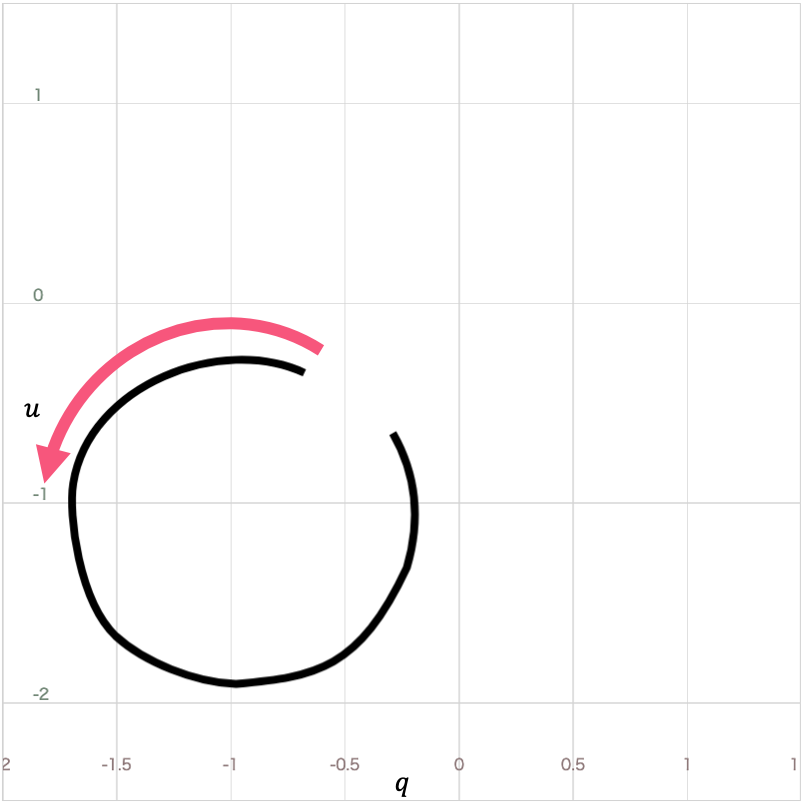
\includegraphics[width=.9\linewidth]{vgtc_journal_latex/figures/QBSSketchwithoutWidth.png}
    \end{minipage}
    \begin{minipage}{0.49\linewidth}
        \centering
        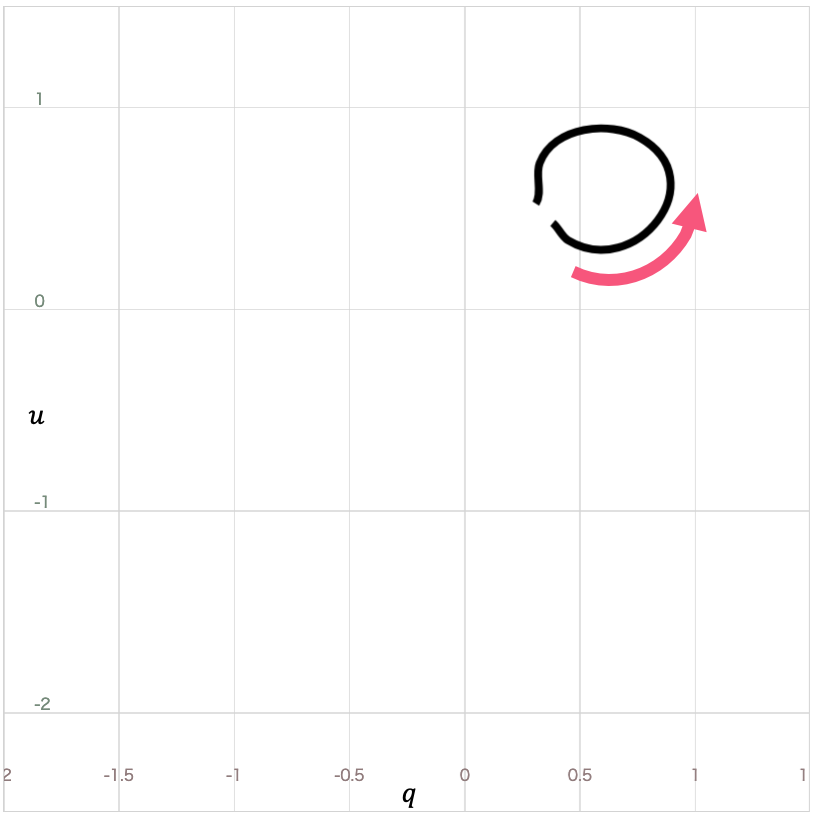
\includegraphics[width=.9\linewidth]{vgtc_journal_latex/figures/QBSResultQuerywithoutWidth.png}
    \end{minipage}
    \begin{minipage}{0.49\linewidth}
        \centering
        \footnotesize{\sf (a)~Hand-drawn sketch query for a small circular pattern.}
    \end{minipage}
    \begin{minipage}{0.49\linewidth}
        \centering
        \footnotesize{\sf (b)~A sketch based on the upper left result in (c). 
        % to extract similar patterns, as shown in (d).
        }
    \end{minipage}
    \begin{minipage}{0.49\linewidth}
        \centering
        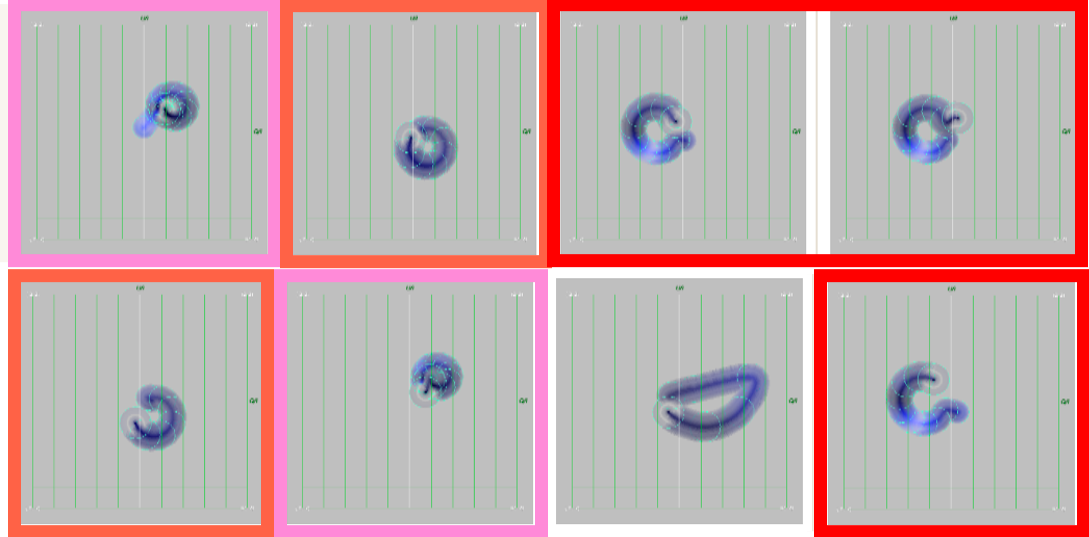
\includegraphics[width=.99\linewidth]{vgtc_journal_latex/figures/QBSResultsHanddrawn.png}\\
        \footnotesize{\sf (c)~Results for the query in (a).}
    \end{minipage}
    \begin{minipage}{0.49\linewidth}
        \centering
        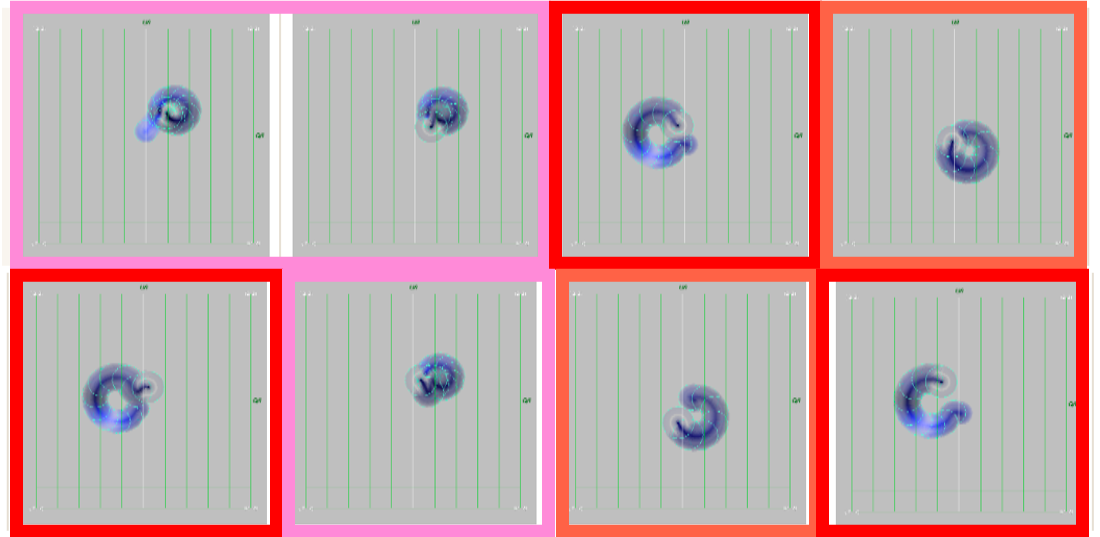
\includegraphics[width=.99\linewidth]{vgtc_journal_latex/figures/QBSResultsResultQuery.png}\\
        \footnotesize{\sf (d)~Results for the query in (b).}
    \end{minipage}
    \caption{QBS results for our synthetic dataset in Fig.~\ref{fig:synthesisData}.
        %The outline color corresponds to the color in \autoref{fig:synthesisData}~(b).
        With a hand-drawn sketch in (a), an unexpected result is highly ranked (white outline) in (c). 
        With a sketch based on actual data values (b), no unexpected results appear, as illustrated in (d).
        % Upon further refinement of the initial sketch to more closely resemble actual data values (b), no unexpected results appear anymore.
        }
    \label{fig:QBSDemodata}
\end{figure}
%
\textsf{Experimental results.\ } We demonstrated the effectiveness of our QBS interface with our synthetic dataset.
%To demonstrate the effectiveness of our QBS interface,
%we have applied QBS to the synthesis data.
%To find out the time intervals with a small circular pattern,
First, we made a query with the sketch shown in Fig.~\ref{fig:QBSDemodata}~(a) to extract time intervals with small circular patterns. 
The sketch pad plane corresponds to the Stokes plane and, for simplicity, the stroke width is not used.
To detect time intervals with a similar shape but different positions or scales, we used the normalization and polar coordinates option.
% Due to the small size of the synthetic dataset, we set the sliding window step size to 2.
Fig.~\ref{fig:QBSDemodata}~(c) shows the top eight results of our QBS method for the query in (a).
The outline color of each thumbnail image matches the color of the corresponding circular pattern in Fig.~\ref{fig:synthesisData}~(b).
% We enclose the results that include the small circular pattern in rectangles 
% The outline color of the individual results corresponds to the colors used in the circular patterns in
% whose color corresponds to the colors used in the circular patterns in \autoref{fig:synthesisData}~(b).
All three time intervals highlighted in red in Fig.~\ref{fig:synthesisData}~(b) were properly extracted.
Nevertheless, an unexpected result (i.e., the thumbnail with no outline color in Fig.~\ref{fig:synthesisData}~(c)) was highly ranked as a candidate similar to the input pattern due to the ambiguities of a hand-drawn sketch.
We address this problem by incorporating fact-guided querying (see Section~\ref{sec:factDrivenQuerying}). 

%
\subsection{Query Matching Algorithm}\label{sec:matchingAlgorithm}
\begin{figure}[tb]
    \begin{minipage}{0.62\linewidth}
        \centering
        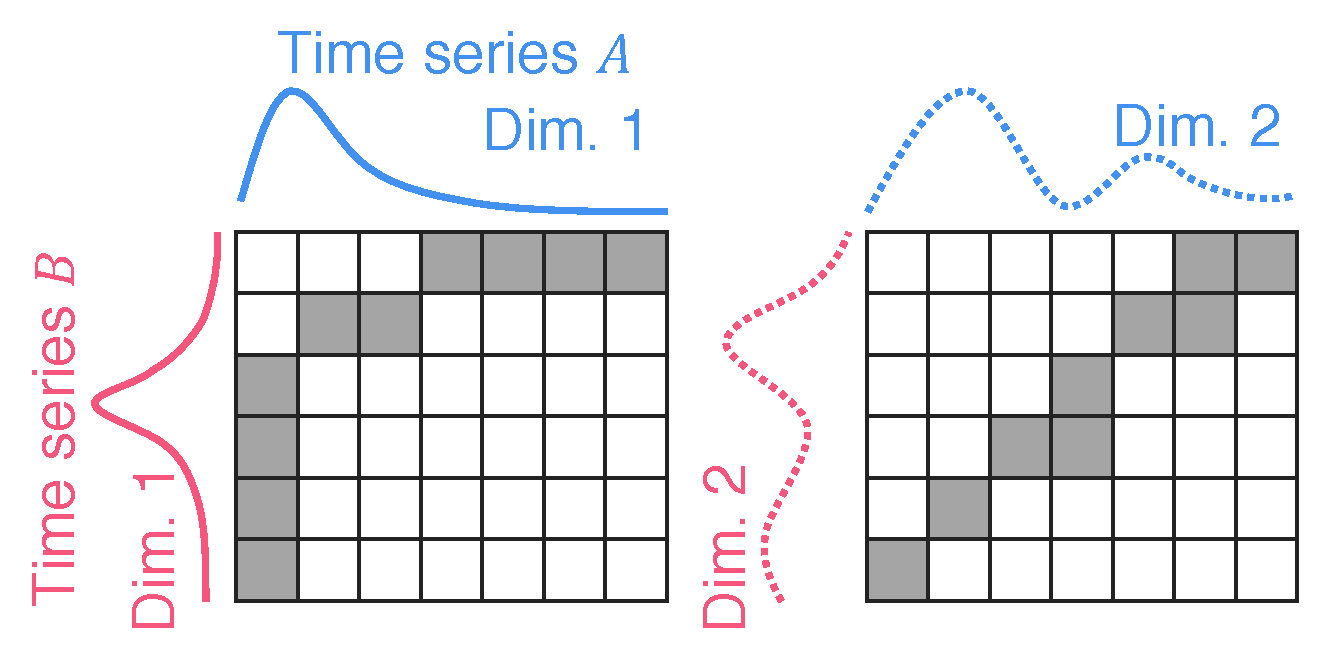
\includegraphics[width=.95\linewidth]{vgtc_journal_latex/figures/DTWI.pdf}\\
    \end{minipage}
    \begin{minipage}{0.37\linewidth}
        \centering
        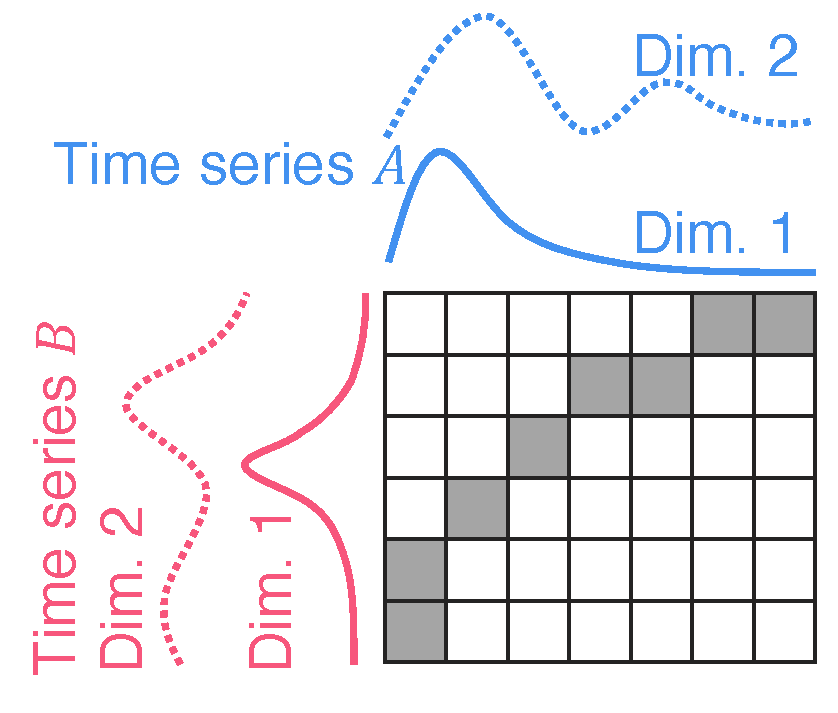
\includegraphics[width=.95\linewidth]{vgtc_journal_latex/figures/DTWD.pdf}\\
    \end{minipage}
    \begin{minipage}{0.62\linewidth}
        \centering
        \footnotesize{\sf(a)~${\rm DTW}_{\rm I}$}
    \end{minipage}
    \begin{minipage}{0.37\linewidth}
        \centering
        \footnotesize{\sf(b)~${\rm DTW}_{\rm D}$}
    \end{minipage}
    \caption{DTW options for dealing with multi-dimensional data.
    ${\rm DTW}_{\rm I}$ warps each dimension independently, whereas all dimensions are warped dependently in ${\rm DTW}_{\rm D}$.}
    \label{fig:DTW}
\end{figure}
%
There are many different methods to compute the distance between two time series, such as the Euclidean distance, uniform scaling, or dynamic time warping (DTW)~\cite{Berndt1994}.
TimeTubesX uses DTW
because it aligns two time series elastically and thus supports the comparison of time series with different lengths.
Additionally, it can compute the distance between two time series that are similar, but locally out of phase.
%more intuitively even if they are out of phase in the time direction. 
According to Eichmann and Zgraggen~\cite{Eichmann2015}, the DTW similarity measurement seems to most closely match human perception.
There are multiple solutions for dealing with multi-dimensional data in DTW. 
TimeTubesX implements two options, ${\rm DTW}_{\rm I}$ (independent) and ${\rm DTW}_{\rm D}$ (dependent), both based on the work of Shokoohi-Yekta et al.~\cite{Shokoohi-Yekta2015}.
%${\rm DTW}_{\rm Independent}$ (${\rm DTW}_{\rm I}$) and ${\rm DTW}_{\rm Dependent}$ (${\rm DTW}_{\rm D}$). 
%The ideas come from Shokoohi-Yekta et al.~\cite{Shokoohi-Yekta2015}.

${\rm DTW}_{\rm I}$ computes the distance between two time series for each dimension of the data separately (see Fig.~\ref{fig:DTW}~(a)). In the final step, it adds up all those individual distances to the final distance measure.
%${\rm DTW}_{\rm I}$ makes each dimension of time series warp irrespective of other dimensions and then cumulates the distances of all dimensions, as illustrated in \autoref{fig:DTW}~(a).
% ${\rm DTW}_{\rm I}$ defines the distance between two time series as a cumulative distance of all dimensions in the time series.
% In other words, it makes each dimension warp irrespective of other dimensions, as illustrated in \autoref{fig:DTW}~(a).
Consequently, this approach focuses more on the similarity of each dimension and less on correlations between different dimensions.
%Consequently, this takes more account not of correlations among dimensions but of similarity of each dimension.
% Consequently, ${\rm DTW}_{\rm I}$ regards time intervals each of whose dimensions has a similar time variation pattern to the input pattern as 
% Consequently, the time variation of each dimension looks similar, 
% but correlations among dimensions may decrease.
% wrong: first accumulates the signal from all dimensions for each time series individually, and then computes the distance between those two accumulated time series (see \autoref{fig:DTW}~(b)).
${\rm DTW}_{\rm D}$, on the other hand, computes the distance between two data samples directly over all dimensions (i.e., as Euclidean distance in $n$-dimensional space), as seen in Fig.~\ref{fig:DTW}~(b).
Therefore, this method focuses more on correlations among the different dimensions of a time series and less on the similarities of individual dimensions. 
%takes more account of correlations among dimensions than similarity of each dimension.
By default, our system uses ${\rm DTW}_{\rm D}$ because correlations among variables are significantly more important for blazar behavior analysis.

We use a sliding window approach in our matching algorithm.
%, the interactive feature extraction picks up a time interval from long-term data 
%and then computes the distance between the input query and the time interval according to the selected option.  
Users can set the window size and the step size of the sliding window and also set a constraint on the largest allowed temporal shift (i.e., warping window size)
% The warping window size determines the largest allowed temporal shift 
in the process of finding the best alignment between the query and time series.
Users can specify these parameters at the bottom of the query specification panel in Fig.~\ref{fig:UIFeatureExtraction}~(A).
Note that multiple time intervals with different lengths but including the same time points can be presented in the extraction results (see Fig.~\ref{fig:QBEDemodata} and Fig.~\ref{fig:QBSDemodata}~(c) and (d)). %because of the use of a sliding window approach.
The timelines in Fig.~\ref{fig:UIFeatureExtraction}~(C) help users recognize such time intervals. 
% Users can identify the groups of the extraction result by giving a glance at the timeline.

Normalization and polar coordinates options enable a fuzzy pattern search.
%The Normalization option and polar coordinates option realize fuzzy pattern search.
The normalization option triggers the system to normalize a query and time intervals into the range of $[0, 1]$.
Subsequently, the pattern search places great significance on the \emph{shape} of the time variations, whereas the actual value ranges will be ignored.
With the polar coordinates option, 
$q(t)$ and $u(t)$ are converted into polar coordinates ($r-\theta$ domain) before computing similarities.
Subsequently, the pattern search with the normalization and polar coordinates options will also be able to extract patterns rotating around the origin of the Stoke plane.

%
%
\subsection{Fact-Guided Querying}\label{sec:factDrivenQuerying}
To support quick and iterative query refinement, TimeTubesX allows users to re-utilize individual extraction results as an input for follow-up queries, a process we termed \emph{fact-guided querying}.
% We call this \emph{fact-driven querying},  
% since it allows users to easily search for time intervals similar to actual data measurements, implying that it makes it easy for users to find common features.
By iteratively updating a query, users can, in a step-by-step manner, identify more observable time intervals that reflect their intentions.
% In other words, the feature extraction and visual query interface realizes a self-organizing query refinement.
% With a refined query, users can find more observable time intervals which reflect their intentions more. 
Therefore, fact-guided querying contributes immensely to drilling-down into data as a part of the visual exploration framework of TimeTubesX in Fig.~\ref{fig:framework}.
In QBE, users can switch variables used in the matching process and modify the time range of the query, while in QBS, users can adjust the scale, shape, and axis of the input query or add further filtering constraints.
% initial interesting time intervalを見つける手間を省いたり?ユーザの意図をより反映したtime intervalに基づいてクエリを作成したり?白紙からスケッチを書かないで、実際の値に基づいて任意のスケッチを作成したりできる
Thus, it helps users perform further pattern searches based on the interesting time interval found in the previous process or create a sketch-based query from references to actual data measurements instead of from a blank sketch pad.
% not from a blank sketch pad but with reference to actual data measurements.

Our system allows users to build a fact-guided query with simple interactions, i.e.,
dragging an extraction result either into the QBE interface (part (2) in Fig.~\ref{fig:querySpecificationPanel}~(B)) or into the sketch pad of the QBS interface (part (3) in Fig.~\ref{fig:querySpecificationPanel}~(C)).
%
%Due to the fact-driven querying function, they can 
%In particular, when changing the axis of the sketch pad, 
%the sketch is automatically updated with reference to the selected result.
%The sketch is 2D, but multi-dimensional data is stored internally as a vital part of a query.


\textsf{Experimental results.\ } We illustrated the usefulness of the fact-guided querying approach with our synthetic dataset.
As discussed in Section~\ref{sec:QBS}, 
hand-drawn sketch queries, such as Fig.~\ref{fig:QBSDemodata}~(a), work well for finding time intervals with a specific feature,
but ambiguities of hand-drawn sketches may sometimes lead to unexpected results, as shown in (c).
%
% \autoref{fig:QBSDemodata}~(a) shows an initial hand-drawn query. %and search for time intervals with a similar feature.
If the extraction results for the query in (a) sufficiently represent users' intentions, one of the results can be used as an input to refine results of the next visual query.
%When we find time intervals which sufficiently validate our intention, we can use the one of the results for yet another query of the visual query.
% For the query in (b), 
We chose the top left result of (c) and used it as an input to our QBS method, as shown in (b). 
%and converted it for a query in QBS.
The sketch pad plane in (b) coincides with the Stokes plane.
Thereafter, we ran QBS in the same parameter settings as the example in Section~\ref{sec:QBS}.
As shown in the top eight extraction results in (d),  % of QBS with the query in (b).
this refined query in (b) no longer produces any highly-ranking outliers or unexpected results.
% does not result in highly ranking any outliers or unexpected results any longer.
%As the red rectangles illustrate,
%unexpected results were not highly ranked any longer.
%The application examples in \autoref{fig:QBSDemodata} illustrate that the fact-driven querying effectively works for the query refinement.



% \begin{figure}[tb]
%     \centering
%     \includegraphics[width=.99\linewidth]{images/GUI.pdf}
%     \caption{User interface of the interactive feature extraction. (a)~Query specification panel; (b)~Parameters for ranking, filtering, and displaying extraction results and a histogram summarizing distance distribution of extraction results; (c)~The timeline overviewing displayed extraction results; (d)~Detail information panel for a selected result; (e)~A collection of thumbnails for extraction results.}
%     \label{fig:UIFeatureExtraction}
% \end{figure}
% \begin{figure}[tb]
%     \centering
%     \begin{minipage}{0.6\linewidth}
%         \centering
%         \includegraphics[width=.99\linewidth]{images/QBEMenuLabel.png}
%     \end{minipage}
%     \begin{minipage}{0.39\linewidth}
%         \centering
%         \includegraphics[width=.97\linewidth]{images/QBSMenuLabel.png}
%     \end{minipage}
%     \begin{minipage}{0.6\linewidth}
%         \centering
%         \footnotesize{\sf (a)~Query-by-example.}% (1)~Panels for specifying ROI from TimeTubes view or scatterplots view; (2)~A 3D tube for selected time interval.}
%     \end{minipage}
%     \begin{minipage}{0.39\linewidth}
%         \centering
%         \footnotesize{\sf (b)~Query-by-sketch.}% (1)~Sketch pad for drawing a query; (2)~A popup panel for filter constraints assignment; (3)~Parameters for controlling the sketch pad and sketch stroke.}
%     \end{minipage}
%     \caption{Query specification panel in the interactive feature extraction (Fig.~\ref{fig:UIFeatureExtraction}~(a)).}
%     \label{fig:QuerySpecification}
% \end{figure}


% Fig.~\ref{fig:UIFeatureExtraction} shows the designate user interface, 
% where QBS option is selected.
% The users are allowed to choose either option of the visual query and specify a query in part (a).
% This query specification panel in part (a) with each option of the visual query is illustrated in Fig.~\ref{fig:QuerySpecification}.
% After running the similarity search, 
% the system displays extraction results according to the parameteres in part (b), 
% such as preferred order of results, threshold for results, and the number of displayed results.
% A histogram summarizing the distance distribution of the extraction results appears in part (b),
% which is helpful for the users to decide how many results to show.
% By adjusting the gray area on the histogram,
% the users can alter the number of the displayed results. 
% The timeline in part (c) overviews the location of the extraction results,
% which enables the users to understand temporal distributions of the results.
% Detail information of the result, such as limit timestamps of the time interval and the distance between the query and time interval, will appear in part (d)
% by selecting a result from the collection of thumbnails in part (e).

% QBE gives a kind of flexibility to a selected example.

% Such flexibility makes it easier for the users to reflect their intentions to the example.

% The task \textbf{T4} is effectively supported by QBE.
% Moreover, \textbf{T5} can also be supported by using a normalization option and polar coordinates option.

% Users can find out time intervals with similar shapes to the query but with different sizes.

% With the combination of both options,
% the users can also find out time intervals at different positions from the query.

    % \begin{minipage}{0.55\linewidth}
    %     \centering
    %     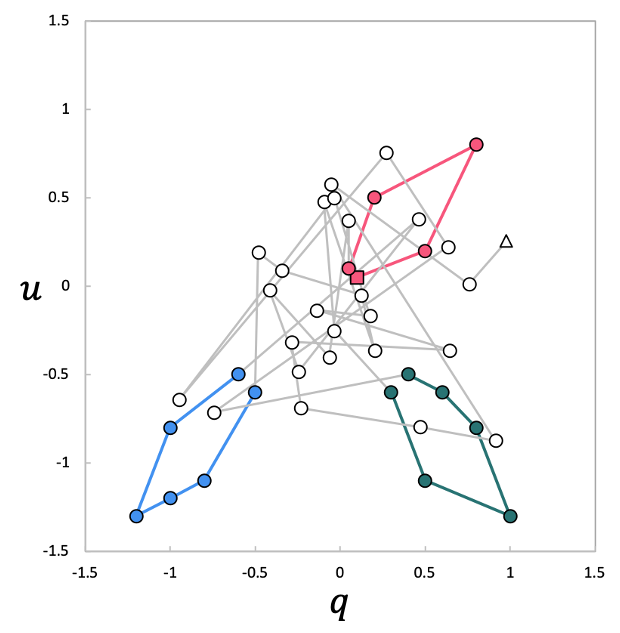
\includegraphics[width=.99\linewidth]{vgtc_journal_latex/figures/QBEdemodataStokes.png}
    % \end{minipage}
    % \begin{minipage}{0.44\linewidth}
    %     \centering
    %     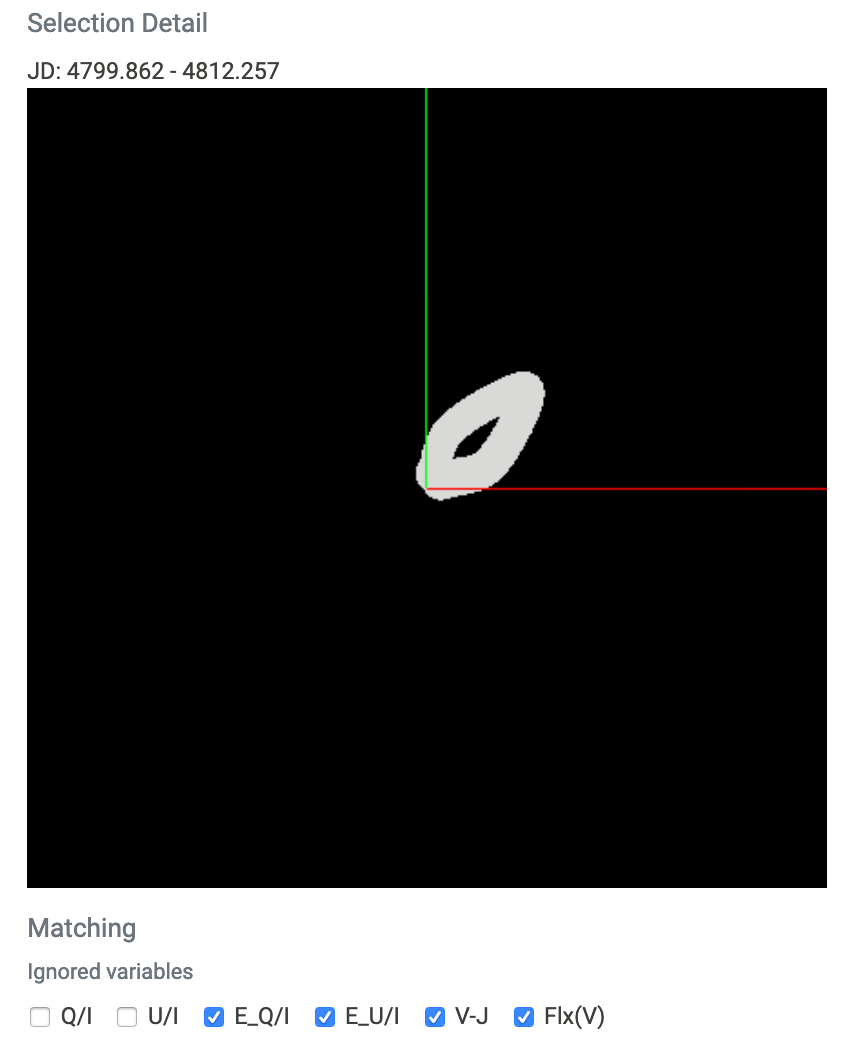
\includegraphics[width=.99\linewidth]{vgtc_journal_latex/figures/QBEdemodataQuery.png}
    % \end{minipage}\\
    % \begin{minipage}{0.55\linewidth}
    %     \centering
    %     \footnotesize{\sf (a)~The data on the Stoke plane.}
    % \end{minipage}
    % \begin{minipage}{0.44\linewidth}
    %     \centering
    %     \footnotesize{\sf (b)~Selected time interval.}
    % \end{minipage}\\
    
    % \footnotesize{\sf (c)~Results of QBE with the query in (a).}
    

% \begin{figure}[tb]
%     \centering
%     \includegraphics[width=.99\linewidth]{images/QBSMenuLabel.png}
%     \caption{Query specification in the query-by-sketch. (a)~Sketch pad. (b)~Filter constraint assignment. (c)~Parameter setting for the sketch.}
%     \label{fig:QBS}
% \end{figure}

% It is obvious that QBS supports \textbf{T5}. 


% DTW is a common algorithm for measuring similarity between two time series.
% Why dynamic time warping?

% When comparing two time-dependent, multi-dimensional data $Q$ and $C$ with $M$ dimensions, %whose length is $l_Q$ and $l_C$ respectively,
% the distance (${\rm DTW}_{\rm I} (Q, C)$) between two time series is expressed by the following equation:
% \begin{eqnarray}
% \label{equ:distanceDTWI}
%     {\rm DTW}_{\rm I} (Q, C) = \sum_{m = 1}^{M}{\rm DTW}(Q_m, C_m).
%     % d(q_{i, m}, c_{j, m}) = \sqrt{(q_{i, m} - c_{j, m})^2}
% \end{eqnarray}

% The following equation computes the distance (${\rm DTW}_{\rm D} (Q, C)$) between two time series $Q$ and $C$:
% \begin{eqnarray}
% \label{equ:distanceDTWD}
%     {\rm DTW}_{\rm D} (Q, C) = {\rm DTW}(\{Q_1, Q_2, \cdots, Q_M\}, \{C_1, C_2, \cdots, C_M\}).
%     % d(q_{i, m}, c_{j, m}) = \sqrt{(q_{i, m} - c_{j, m})^2}
% \end{eqnarray}

% The following part explains DTW for multi-dimensional data.
% Data $Q$ and $C$ is a collection of $M$ time series whose length is $l_Q$ and $l_C$ respectively:
% \begin{eqnarray*}
%     Q_1 &=& q_{1, 1}, q_{2, 1}, \cdots , q_{l_Q, 1} \\
%     Q_2 &=& q_{1, 2}, q_{2, 2}, \cdots , q_{l_Q, 2} \\
%     \cdots \\
%     Q_M &=& q_{1, M}, q_{2, M}, \cdots , q_{l_Q, M}
% \end{eqnarray*}
% \begin{eqnarray*}
%     C_1 &=& c_{1, 1}, c_{2, 1}, \cdots , c_{l_C, 1} \\
%     C_2 &=& c_{1, 2}, c_{2, 2}, \cdots , c_{l_C, 2} \\
%     \cdots \\
%     C_M &=& c_{1, M}, c_{2, M}, \cdots , c_{l_C, M}
% \end{eqnarray*}
% For ${\rm DTW}_{\rm I}$, we construct $M$ $l_Q-$by$-l_C$ distance matrix, where the $(i_m, j_m)$ element is the distance $d(q_{i, m}, c_{j, m})$ between two points $q_{i, m}$ and $c_{j, m}$.
% \begin{eqnarray}
% \label{equ:distanceDTWI}
%     d(q_{i, m}, c_{j, m}) = \sqrt{(q_{i, m} - c_{j, m})^2}
% \end{eqnarray}
% The definition of the cumulative distance $D(i, j)$ of ${\rm DTW}_{\rm I}$ is same as DTW for single-dimensional time series.
% \begin{eqnarray}
% \label{equ:DDTWI}
%     D_m(i, j) = d(q_{i, m}, c_{j, m}) 
%     + \min \left\{
%     \begin{array}{l}
%         D_m(i - 1, j - 1), \\
%         D_m(i - 1, j), \\
%         D_m(i, j - 1)
%     \end{array}
%     \right\}
% \end{eqnarray}
% The $(l_Q, l_C)$ element in the distance matrix represents the maximum distance between $Q$ and $C$.
% In the case of ${\rm DTW}_{\rm I}$, therefore, the distance between two data $DTW_I$ is as follows:
% \begin{eqnarray}
% \label{eqn:DTWI}
%     DTW_I = \sum_{m=1}^{M} D_m(l_Q, l_C).
% \end{eqnarray}

% For ${\rm DTW}_{\rm D}$, we construct a $l_Q-$by$-l_C$ distance matrix, where the $(i_m, j_m)$ element is as follows:
% \begin{eqnarray}
% \label{eqn:distanceDTWD}
%     d(q_i, c_j) = \sum_{m = 1}^{M} \sqrt{(q_{i, m} - c_{j, m})^2}.
% \end{eqnarray}
% The cumulative distance $D(i, j)$ depends on the sum of distances computed in Equation \ref{eqn:distanceDTWD}.
% \begin{eqnarray}
% \label{equ:DDTWD}
%     D(i, j) = d(q_{i}, c_{j}) 
%     + \min \left\{
%     \begin{array}{l}
%         D(i - 1, j - 1), \\
%         D(i - 1, j), \\
%         D(i, j - 1)
%     \end{array}
%     \right\}
% \end{eqnarray}
% Finally, the maximum distance between two data $DTW_D$ is as follows:
% \begin{eqnarray}
% \label{eqn:DTWD}
%     DTW_D = D(l_Q, l_C).
% \end{eqnarray}

% \begin{figure}[tb]
%     \centering
%     \includegraphics[width=.99\linewidth]{images/ResultQuerying.png}
%     \caption{Users are allowed to re-utilize a result as a key for query-by-sketch.}
%     \label{fig:resultQuerying}
% \end{figure}

% By normalizing the query or using polar coordinates in the matching process, 
% our system can identify time intervals with similar shapes but different scales or those transformed, too.

% It is a chief card for \textbf{T4}.
\section{Visual Exploration of Query Results}\label{sec:otherFunctions}
In addition to the feature and pattern detection methods described in Sections~\ref{sec:automaticExtraction} and \ref{sec:visualQuery}, TimeTubesX includes powerful visual comparison and annotation features for further analysis of blazar data.

%the present analysis functions for extracting features in a synergetic way,
%we introduce several auxiliary functions into TimeTubesX.

\subsection{Visual Comparison of Query Results}
An essential feature for analysis of blazar datasets is the user's ability to compare query results---not just within a single query but also to previous query results. 
For example, when users find that a specific feature frequently appears in a certain time period,
they might want to investigate whether any other features also frequently appear in the same time period.
Therefore, TimeTubesX can juxtapose the results of different queries
by loading query results that were previously saved as a JSON file.
%
%They can store the query information with the annotation function, but extraction results are automatically overwritten every time they run a new query.
% Furthermore, users can save and load query results to and from disk, as a JSON file, to allow comparisons even between different sessions and users.
%, users can export extraction results as a JSON file and import the file.
When importing a file, the stored results are mapped to a new timeline that is arranged as a juxtaposed view below the original timeline.
%in different colors from the current extraction results.
Hovering over marks on the timeline allows users to see detailed information about specific results.
Additionally, users can re-use or review the settings of the previous query, such as the selected time period or the variables assigned to the sketch pad (see Fig.~\ref{fig:UIFeatureExtraction}~(F)).
%If needed, they can reuse the previous query.

% \subsection{Annotations of time steps, queries, and query results}
\subsection{Annotations of Queries and Query Results}
%
To enable efficient collaboration between astronomers and to facilitate keeping track of analyses between different sessions, TimeTubesX supports detailed annotations for query results.
% Annotations allow users to document their analysis process and to share their results with others.
% queries, query results, and time spans of interest.
%
%The users can annotate extracted results. 
Users can access any annotations even after exiting and restarting the application because annotations are stored in the local storage of the web browser. 
To share annotations with other users, annotations can be exported as a single JSON file. 
%The users are allowed to export the annotations as a JSON file, which will make it easy to share insights among the colleagues.
The system stores the annotation's timestamp, username, comment, and dataset, as well as detailed information about the query and query results.
Users can see all of their annotations in a table view or a single annotation by clicking on a marker with the selected label color in the TimeTubes and scatterplots views.
They can also re-use any query saved in an annotation by simply clicking on it. %just by selecting an annotation.

Annotations help users highlight interesting extraction results.
% of the feature and pattern detection.
%
% This is especially important to iteratively refine queries, to exclude those time intervals that do not reflect the user's intentions.
%
%because the feature extraction of TimeTubesX presents candidates for characteristic blazar behaviors or time intervals resembling the input pattern, but time intervals which do not reflect the users' intentions enough might also be included.
Annotating time intervals of interest not only triggers deeper inspection of a specific period 
but also possibly facilitates the discovery of new features such as periodic patterns.






% \begin{figure}[tb]
%     \centering
%     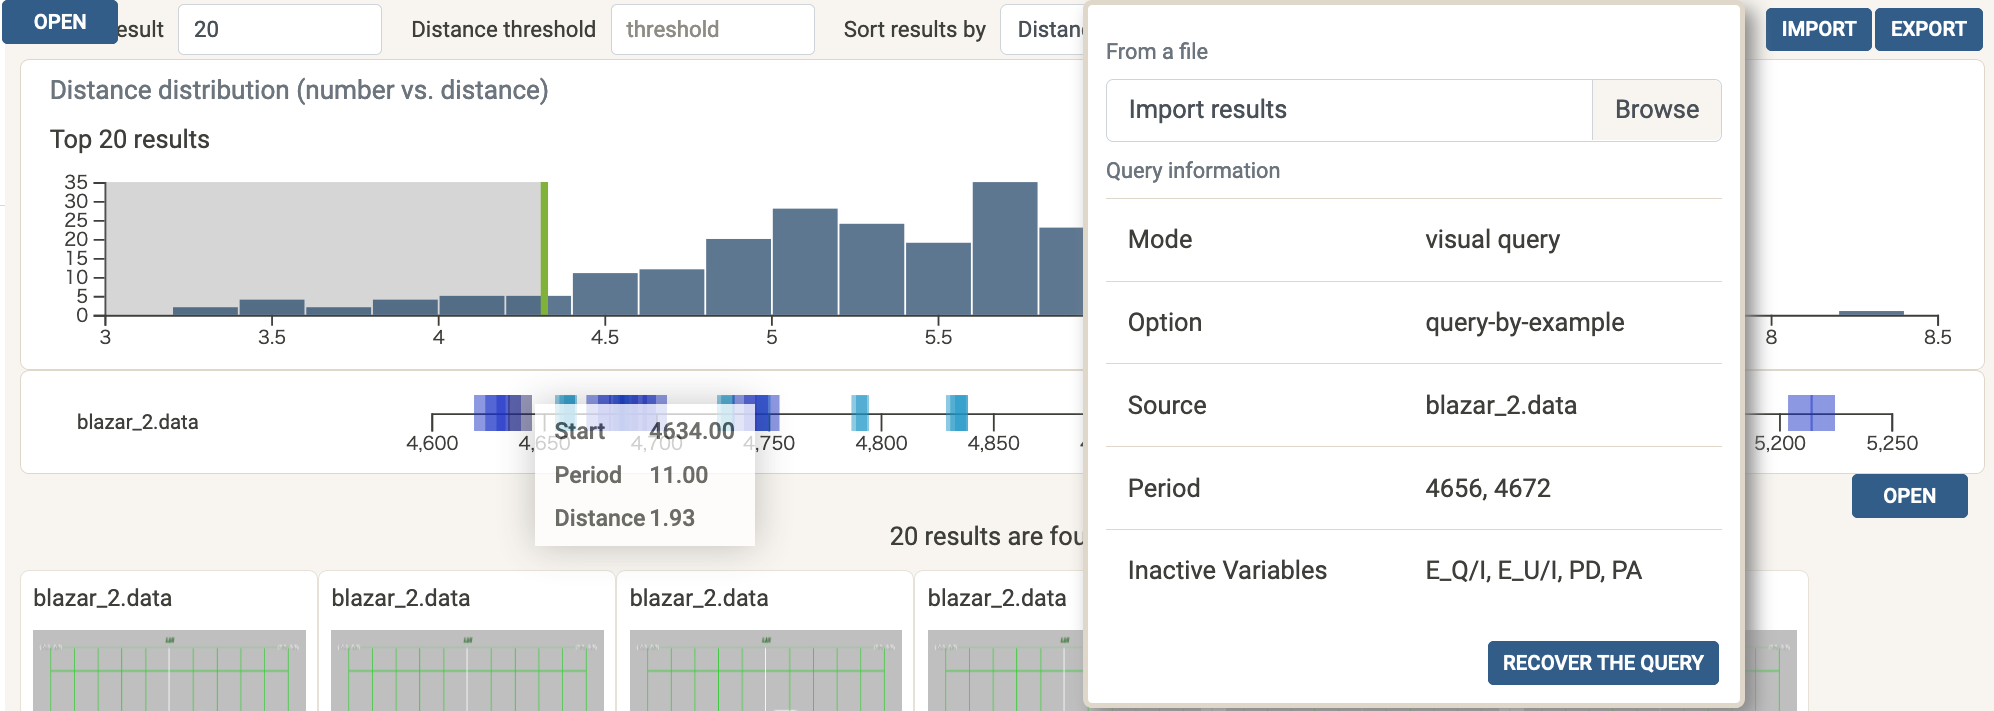
\includegraphics[width=.99\linewidth]{vgtc_journal_latex/figures/resultComparison.png}
%     \caption{Comparing the current extraction results with the previous ones. 
%         Light blue plots indicate the current extraction results, 
%         while dark blue plots do the previous ones.}
%     \label{fig:resultsComparison}
% \end{figure}
% \subsection{Implementation}\label{sec:Implementation}
% TimeTubesX is a browser-based application written in HTML and Javascript.
% We use React.js to build user interfaces and flux.js to manage the application state.
% We also utilize standard libraries such as D3.js~\cite{d3_framework} and paper.js~\cite{paper_framework}.
% TimeTubesX is open-source and running system can be found at \url{https://timetubes.herokuapp.com/}.



\section{Evaluation\label{sec:evaluation}}
TimeTubesX is a browser-based application written in HTML and Javascript.
We use React.js to build user interfaces and flux.js to manage the application states.
We also utilize standard libraries such as three.js~\cite{three_framework}, D3.js~\cite{d3_framework}, and Paper.js~\cite{paper_framework}.
TimeTubesX is open-source (\url{https://github.com/MistletoeNaoko/TimeTubesWeb}), and 
readers can try the running system using our synthetic data at \url{https://timetubes.herokuapp.com/}.

We shared TimeTubesX with four domain experts, three of whom we interviewed for the domain analysis in Section~\ref{sec:domainGoalsandTasks}: the second author of this paper (Astronomer 1), Astronomer 1’s former master course student (Astronomer 2), an assistant professor at Hiroshima University (Astronomer 3), and a postdoctoral researcher at Stanford University (Astronomer 4). Sections \ref{sec:correlate} and \ref{sec:anticorrelate} present two case studies conducted by Astronomer 1, and Section \ref{sec:whatif} discusses the cause of the phenomena presented in Section \ref{sec:anticorrelate}. Section \ref{sec:feedback} reviews qualitative feedback from the four domain experts.
To examine the magnetic field structures in the jets, 
astronomers analyze polarimetric observations. 
Through the analysis of correlations between polarization and intensity, 
they validate multiple hypotheses for the increase in the intensity ($I$). 
In the two case studies, Astronomer 1 used the datasets for the blazar \emph{BL Lac}.
It was empirically noted in \cite{Gaur2014} that the $I$ of \emph{BL Lac} tends to anticorrelate with the polarization degree ($PD$) during a certain period.
On a MacBook Pro 2017 with a 3.5 GHz Intel Core i7 and a 16 GB RAM, it took 1{,}193 ms and 1{,}236 ms to obtain the results outlined in Sections~\ref{sec:correlate} and \ref{sec:anticorrelate}, respectively.

\subsection{Case Study 1: Correlation Patterns of $I$ and $PD$}\label{sec:correlate}
\begin{figure}[tb]
    \centering
    \begin{minipage}{0.49\linewidth}
        \centering
        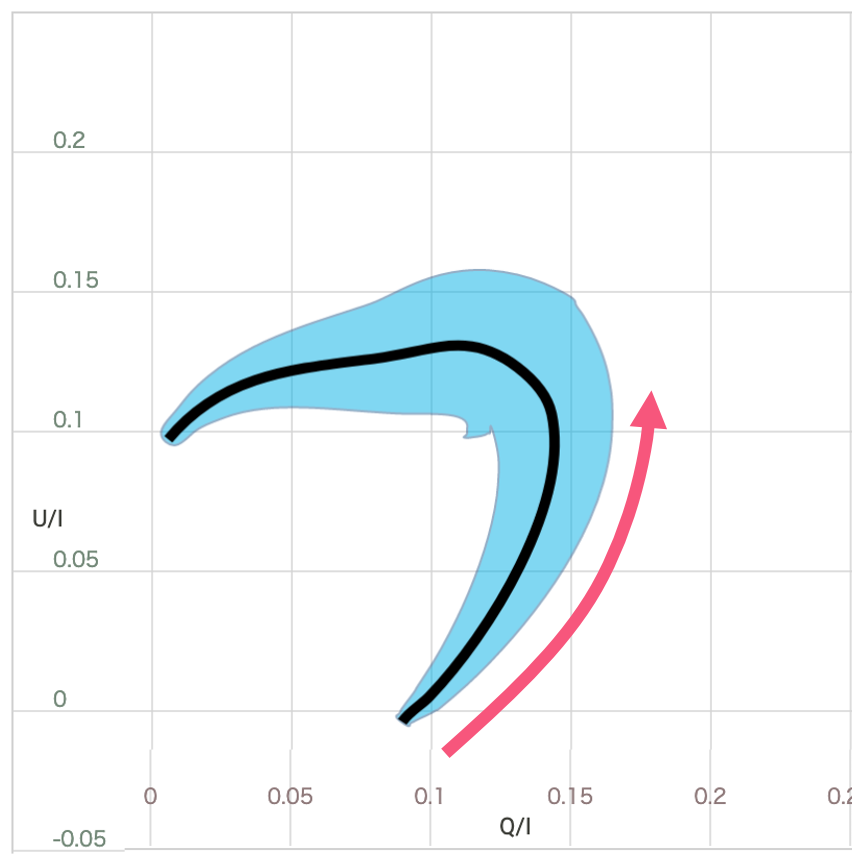
\includegraphics[width=.9\linewidth]{vgtc_journal_latex/figures/QBScorrelate.png}\\
        \footnotesize{\sf(a)~A query for a correlated $I$ and $PD$ variation.}\\
    \end{minipage}
    \begin{minipage}{0.49\linewidth}
        \centering
        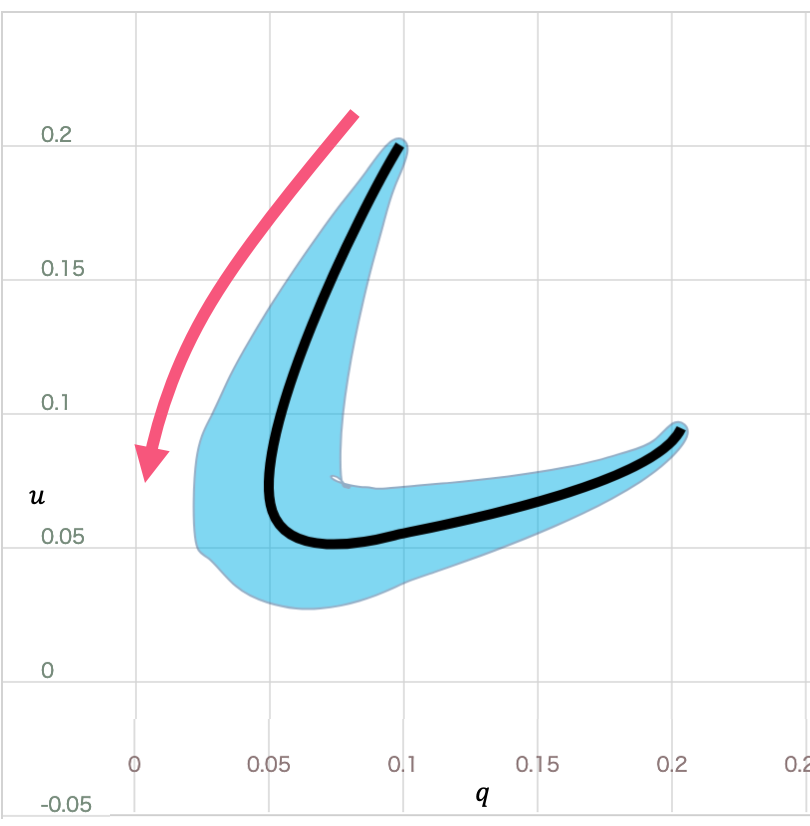
\includegraphics[width=.9\linewidth]{vgtc_journal_latex/figures/QBSanticorrelate.png}\\
        \footnotesize{\sf(b)~A query for an anticorrelated $I$ and $PD$ variation.}\\
    \end{minipage}
    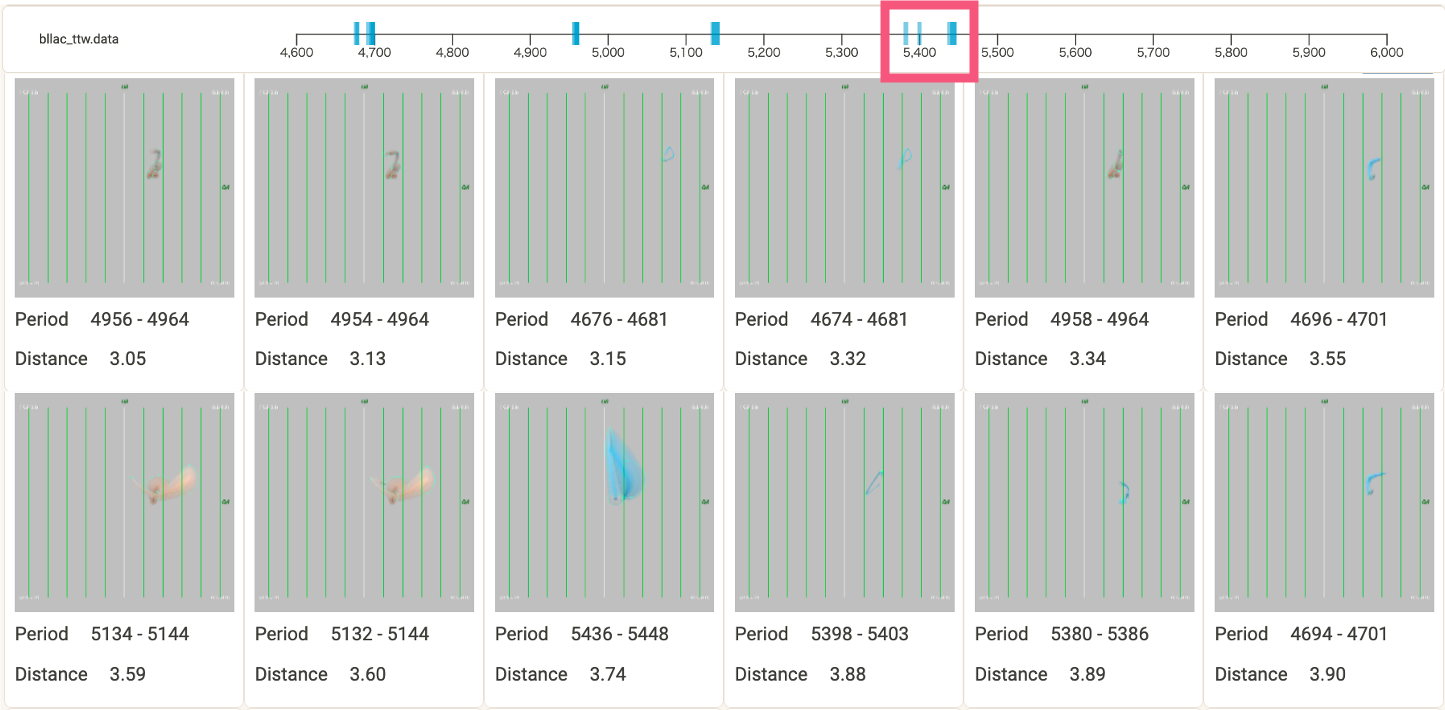
\includegraphics[width=.99\linewidth]{vgtc_journal_latex/figures/correlateResultsLabel14.png}\\
    \footnotesize{\sf(c)~The top twelve time intervals that are similar to the query in (a).}\\
    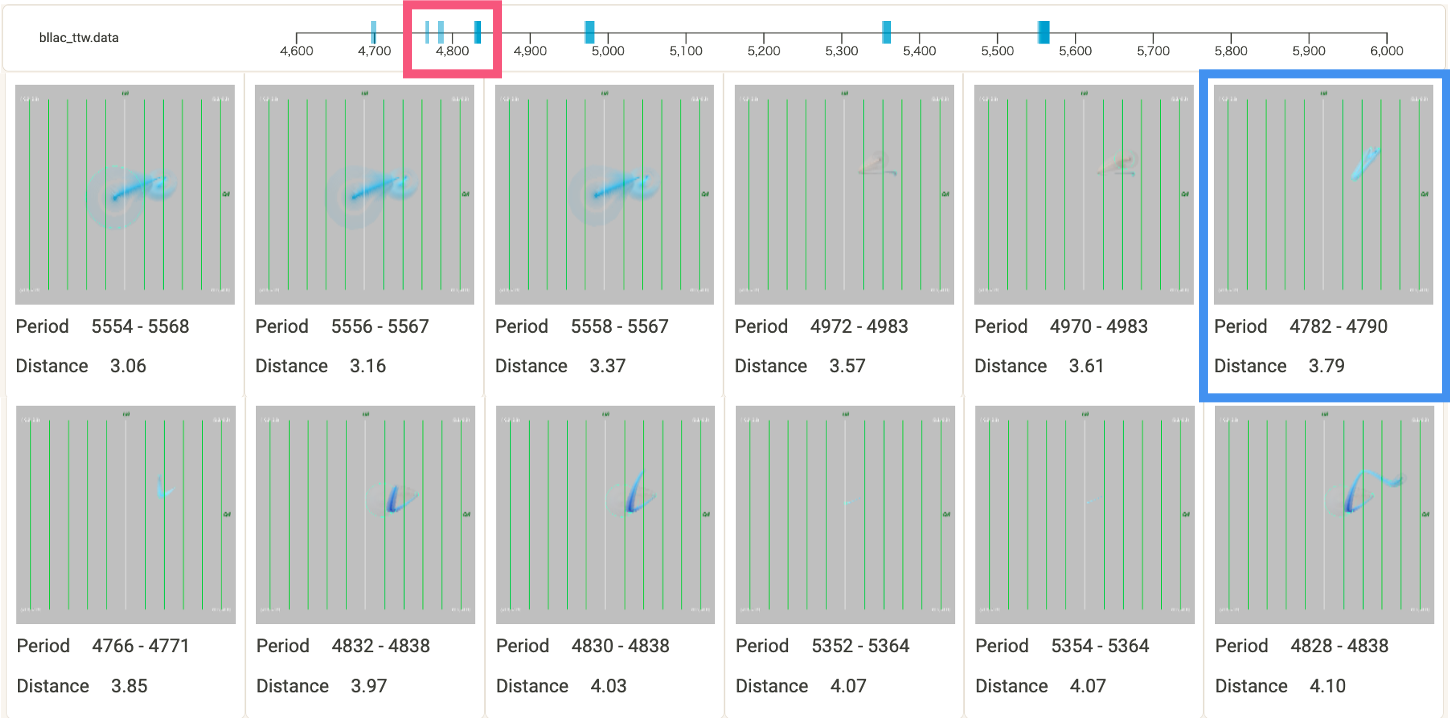
\includegraphics[width=.99\linewidth]{vgtc_journal_latex/figures/anticorrelateResultsLabel14.png}\\
    \footnotesize{\sf(d)~The top twelve time intervals that are similar to the query in (b).}
    \caption{Analysis of the blazar \emph{BL Lac} to investigate correlation patterns between $I$ and $PD$. (a) and (b) are user-drawn sketches. (c) and (d) are the results of QBS with the queries shown in (a) and (b), respectively.}
    \label{fig:EvaluationQueryResults}
\end{figure}
%
Astronomer 1's goal in these case studies was to identify global statistical features of the period of interest and to build a hypothesis of correlations between the time variations of $I$ and $PD$.
To achieve this goal, he had to meticulously analyze correlations between $I$ and $PD$ in the entire time period and many short time intervals within that period.
However, it seemed difficult to manually examine each of the short time intervals.
Therefore, he decided to utilize QBS to investigate correlation patterns in a long-term observation dataset.

First, he formulated a hypothesis that an increase in $I$ tends to correlate with an increase in $PD$ in \emph{BL Lac}.
To validate this hypothesis and examine how frequently such behavior appears, he sketched the query shown in Fig.~\ref{fig:EvaluationQueryResults}~(a), 
where the $x$ and $y$ axes express $q$ and $u$, respectively, 
and the stroke width represents $I$.
Therefore, the input sketch indicates a pattern 
that $I$ gradually increases and then decreases in a way that is correlated to $PD$.
To extract time intervals with a similar shape but different position or different scale, he used the normalization and polar coordinates options. 
To avoid missing short events, he set the warping window size and the sliding window size to 0 and 2, respectively.

Fig.~\ref{fig:EvaluationQueryResults}~(c) shows the top twelve results of the query sketched in (a).
The timeline at the top of (c) illustrates 
that the extracted time intervals seem to be distributed over the entire dataset.
However, in the period from $[5{,}350, 5{,}450]$ (enclosed by a red rectangle in (c)), 
the input pattern seems to occur more frequently than in other periods.
Visiting all time intervals in this period individually and analyzing them in the TimeTubes view,
some of them include the correlation pattern in (a),
but others do not.
Thus, he concluded that the input correlation pattern does not frequently occur in that period.
The reason for this misclassification could be that our system, when using the normalization option, detects time intervals with a relatively small variation of $I$ as well.
However, he was still highly pleased with TimeTubesX, as it allowed him to quickly identify a relatively small number of time intervals that he could then examine in more detail.

\subsection{Case Study 2: Anticorrelation Patterns of $I$ and $PD$}\label{sec:anticorrelate}
Astronomer 1 also noticed that the variation in $I$ tends to anticorrelate with that in $PD$.
To detect time intervals with such anticorrelated $I$ and $PD$ patterns, he drew another query (Fig.~\ref{fig:EvaluationQueryResults}~(b))
where the plane represents the Stokes plane and the stroke width $I$.
The sketch describes a pattern in which $I$ gradually increases and then decreases, while $PD$ shows a negative correlation with $I$. 
He used the same parameters as in Section~\ref{sec:correlate}.

Fig.~\ref{fig:EvaluationQueryResults}~(d) shows the top twelve results of the query shown in (b).
Like in the previous case study, 
extracted time intervals seem to be distributed over the entire dataset.
However, in the period from $[4{,}750, 4{,}850]$ (enclosed by a red rectangle in (d)), 
the input pattern seems to occur more frequently.
Astronomer~1's group previously reported that, statistically, the variation in $I$ anticorrelates with that in $PD$ from the years 2008 to 2010 in \emph{BL Lac}~\cite{Gaur2014}.
However, even in that previous report, they did not analyze short time intervals in the period individually.
By analyzing the extracted time intervals in the period with TimeTubesX, he could verify not only that an increase in $I$ globally tends to co-occur with a decrease in $PD$, 
but also that local peaks of $I$ are correlated with decreases in $PD$.

These case studies with QBS underline the importance of local analysis of short time intervals within a larger time period in addition to a global analysis of the entire period.

\subsection{What-If Scenario Analysis}\label{sec:whatif}
This section explains how astronomers can identify what generally contributes to the $PD$ variation in blazars in a certain time period. 

Astronomers expect that $PD$ variation in a blazar is due to one of the two following hypotheses:
\begin{enumerate}[nosep, label=\textsl{Hypothesis \arabic*}:, ref=\textsl{Hypothesis \arabic*}, align=parleft, leftmargin=*]
    \item \textsl{$total\,flux$ increases (decreases) due to the increase (decrease) in $unpolarized\,flux$};  \label{scenario1}
    \item \textsl{There are two polarized components, and they are perpendicular to each other}. \label{scenario2}
\end{enumerate}
Note that $PD$ can be derived from the amount of $flux$: $PD = \frac{polarized\,flux}{total\,flux}$,
where $total flux = I = polarized\,flux + unpolarized\,flux$.
Astronomers can identify which of the above hypotheses contributes to the decrease in $PD$
by comparing time variations of data samples at the time intervals in the $q - u$ domain and in the $Q-U$ domain,
where $q = Q / I$ and $u = U / I$, as explained in Section~\ref{sec:BlazarData}.
In the case of \ref{scenario1}, the position of a data sample in the $q - u$ domain gradually moves toward the origin ($(q, u) = (0, 0)$),
whereas the position in the $Q-U$ domain does not move toward the origin ($(Q, U) = (0, 0)$)
because only the amount of $total flux$ increases.
On the other hand, in the case of \ref{scenario2}, 
$PD$ decreases due to a flare of another polarized component with $PA$ being perpendicular to the jet direction.
The position of a data sample moves toward the origin both in the $q - u$ domain and in the $Q - U$ domain 
because another polarized component influences the observed $Q$ and $U$ values, 
meaning that $q$ and $u$ (fractional values of $Q$ and $U$) are also influenced.
By comparing the datasets for $(q, u)$ and $(Q, U)$ with the side-by-side option in the visual data fusion~\cite{Fujishiro2018},
the plausibility of these hypotheses can be visually determined.
\begin{figure}[tb]
    \centering
    \includegraphics[width=.8\linewidth]{vgtc_journal_latex/figures/stokesComparisonLabel.png}
    \caption{Comparison of a dataset consisting of $q$ and $u$ (left) and one consisting of $Q$ and $U$ (right) for the time interval $[4{,}782, 4{,}890]$.
    In both images, the position of the data sample goes toward the origin of the domain (lower left), which means that this polarization variation was caused by a decrease in the $PD$ of a different polarized component.}
    \label{fig:comparisonQIUIvsQU}
\end{figure}

The following discussion considers the anticorrelation patterns of $I$ and $PD$, as mentioned in Section~\ref{sec:anticorrelate}.
Astronomer 1 compared a dataset consisting of $q$ and $u$ with one consisting of $Q$ and $U$. The comparison results at the time interval with a blue rectangle displayed in Fig.~\ref{fig:EvaluationQueryResults}~(d) are shown in Fig.~\ref{fig:comparisonQIUIvsQU}.
As the red arrows in Fig.~\ref{fig:comparisonQIUIvsQU} indicate, 
he found that both data samples move toward the origin.
He found similar behavior at all short time intervals in the period $[4{,}750, 4{,}850]$.
Thus, he finally concluded that the negative correlation of $I$ and $PD$ in the period is not due to the increase in $unpolarized flux$ (\ref{scenario1}) but is instead due to the presence of two polarized components (\ref{scenario2}). 

Overall, TimeTubesX greatly facilitated this detailed visual exploration of blazar data. This allowed Astronomer 1 to examine many small time intervals with specific features, which would have been too laborious with previous methods.

\subsection{Qualitative Feedback from Domain Experts}\label{sec:feedback}
Astronomer 2 found that the rotation detection was useful. 
With TimeTubesX's rotation detection functionality, 
he was able to find three unknown rotation behaviors with a shifted rotation center in the blazar \emph{3C 454.3}~\cite{Huang2019}. 
Astronomers 1, 3, and 4 mentioned that the QBS method was especially useful and helpful for validating their high-level hypotheses, as demonstrated in Sections~\ref{sec:correlate} and \ref{sec:anticorrelate}. 
In particular, Astronomers 3 and 4 said that dynamic visual querying could be a powerful tool to examine jet physical processes and behaviors of plasma and magnetic fields under extreme conditions because the method can efficiently address arbitrary variation patterns of polarization, intensity, and color over time. Astronomers 1 and 3 noticed TimeTubesX’s potential for data mining. In particular, Astronomer 3 saw massive potential for mining existing and upcoming large polarization surveys, while Astronomer 1 found that using TimeTubesX will enable astronomers to identify interesting features in short time intervals to an extent that cannot be achieved with conventional methods due to too many short time intervals in a long-term dataset. Furthermore, fact-guided querying was impressive to him because it allows astronomers to refine their sketches based on actual extracted patterns.

\section{Conclusion and future work\label{sec:conclusion}}
We have presented a web-based visual analytics environment, termed TimeTubesX, for the detailed analysis of blazar datasets. %on top of our previous version of TimeTubes.
% Our system incorporates our prior work on 3D visualization of blazar data~\cite{Fujishiro2018} and further provides automatic feature extraction methods and dynamic visual queries that allow users to efficiently identify observable behaviors or recurring features from long-term datasets. 
% We introduced a novel query specification framework for time-dependent, multi-dimensional data. Users can refine a query iteratively to find interesting patterns through a fact-driven querying process.
TimeTubesX has significantly improved astronomers' analysis of 
% multi-dimensional, time-dependent blazar datasets
photometric and polarimetric behaviors of blazars
by providing automatic feature extraction and dynamic visual querying.
It allows astronomers not only to easily locate observable blazar behaviors but also to efficiently find recurring time variation patterns.
TimeTubesX has the potential to allow astronomers to notice short time variation patterns that have not yet been discovered.

% The feature and pattern detection in TimeTubesX still has some limitations.
% % First, our automatic feature extraction allows users to analyze long-term datasets and obtain candidates for characteristic behaviors, but our system cannot distinguish outliers from flares and it can miss rotations that include outliers.
% First, our automatic feature extraction cannot distinguish outliers from flares and it can miss rotations that include outliers.
% In the future, we should take the observation errors into account during the feature extraction processes to alleviate this problem. 
% % We currently do not take the observation errors into account during the feature extraction processes, which would alleviate this problem.
% Second, analyses based on user-driven dynamic visual querying can be biased because the query specification process in QBE and QBS significantly depends on users' experiences and expertise.
% Incorporating deep learning will be able to address this problem by classifying time series in non-biased manner.
% Finally, to give a more effective overview of the results, it would be helpful to cluster the results of a query, similar to the approach by Bernard et al.~\cite{Bernard2010}.

In the future, 
to distinguish outliers from flares and in order not to miss rotations that include outliers,
we should take the observation errors into account during the feature extraction processes. 
Furthermore, we would like to incorporate a deep learning approach to classifying time series data in a non-biased manner because the current query specification process in QBE and QBS significantly depends on users' experiences and expertise.
To give a more effective overview of the results, it will also be helpful to cluster the results of a query. %, similar to the approach by Bernard et al.~\cite{Bernard2010}.
Applying TimeTubesX to multi-dimensional, time-dependent datasets in other domains will likely be yet another part of our future research.


% \IEEEraisesectionheading{\section{Introduction}\label{sec:introduction}}
% % Computer Society journal (but not conference!) papers do something unusual
% % with the very first section heading (almost always called "Introduction").
% % They place it ABOVE the main text! IEEEtran.cls does not automatically do
% % this for you, but you can achieve this effect with the provided
% % \IEEEraisesectionheading{} command. Note the need to keep any \label that
% % is to refer to the section immediately after \section in the above as
% % \IEEEraisesectionheading puts \section within a raised box.




% % The very first letter is a 2 line initial drop letter followed
% % by the rest of the first word in caps (small caps for compsoc).
% % 
% % form to use if the first word consists of a single letter:
% % \IEEEPARstart{A}{demo} file is ....
% % 
% % form to use if you need the single drop letter followed by
% % normal text (unknown if ever used by the IEEE):
% % \IEEEPARstart{A}{}demo file is ....
% % 
% % Some journals put the first two words in caps:
% % \IEEEPARstart{T}{his demo} file is ....
% % 
% % Here we have the typical use of a "T" for an initial drop letter
% % and "HIS" in caps to complete the first word.
% \IEEEPARstart{T}{his} demo file is intended to serve as a ``starter file''
% for IEEE Computer Society journal papers produced under \LaTeX\ using
% IEEEtran.cls version 1.8b and later.
% % You must have at least 2 lines in the paragraph with the drop letter
% % (should never be an issue)
% I wish you the best of success.

% \hfill mds
 
% \hfill August 26, 2015

% \subsection{Subsection Heading Here}
% Subsection text here.

% % needed in second column of first page if using \IEEEpubid
% %\IEEEpubidadjcol

% \subsubsection{Subsubsection Heading Here}
% Subsubsection text here.


% % An example of a floating figure using the graphicx package.
% % Note that \label must occur AFTER (or within) \caption.
% % For figures, \caption should occur after the \includegraphics.
% % Note that IEEEtran v1.7 and later has special internal code that
% % is designed to preserve the operation of \label within \caption
% % even when the captionsoff option is in effect. However, because
% % of issues like this, it may be the safest practice to put all your
% % \label just after \caption rather than within \caption{}.
% %
% % Reminder: the "draftcls" or "draftclsnofoot", not "draft", class
% % option should be used if it is desired that the figures are to be
% % displayed while in draft mode.
% %
% %\begin{figure}[!t]
% %\centering
% %\includegraphics[width=2.5in]{myfigure}
% % where an .eps filename suffix will be assumed under latex, 
% % and a .pdf suffix will be assumed for pdflatex; or what has been declared
% % via \DeclareGraphicsExtensions.
% %\caption{Simulation results for the network.}
% %\label{fig_sim}
% %\end{figure}

% % Note that the IEEE typically puts floats only at the top, even when this
% % results in a large percentage of a column being occupied by floats.
% % However, the Computer Society has been known to put floats at the bottom.


% % An example of a double column floating figure using two subfigures.
% % (The subfig.sty package must be loaded for this to work.)
% % The subfigure \label commands are set within each subfloat command,
% % and the \label for the overall figure must come after \caption.
% % \hfil is used as a separator to get equal spacing.
% % Watch out that the combined width of all the subfigures on a 
% % line do not exceed the text width or a line break will occur.
% %
% %\begin{figure*}[!t]
% %\centering
% %\subfloat[Case I]{\includegraphics[width=2.5in]{box}%
% %\label{fig_first_case}}
% %\hfil
% %\subfloat[Case II]{\includegraphics[width=2.5in]{box}%
% %\label{fig_second_case}}
% %\caption{Simulation results for the network.}
% %\label{fig_sim}
% %\end{figure*}
% %
% % Note that often IEEE papers with subfigures do not employ subfigure
% % captions (using the optional argument to \subfloat[]), but instead will
% % reference/describe all of them (a), (b), etc., within the main caption.
% % Be aware that for subfig.sty to generate the (a), (b), etc., subfigure
% % labels, the optional argument to \subfloat must be present. If a
% % subcaption is not desired, just leave its contents blank,
% % e.g., \subfloat[].


% % An example of a floating table. Note that, for IEEE style tables, the
% % \caption command should come BEFORE the table and, given that table
% % captions serve much like titles, are usually capitalized except for words
% % such as a, an, and, as, at, but, by, for, in, nor, of, on, or, the, to
% % and up, which are usually not capitalized unless they are the first or
% % last word of the caption. Table text will default to \footnotesize as
% % the IEEE normally uses this smaller font for tables.
% % The \label must come after \caption as always.
% %
% %\begin{table}[!t]
% %% increase table row spacing, adjust to taste
% %\renewcommand{\arraystretch}{1.3}
% % if using array.sty, it might be a good idea to tweak the value of
% % \extrarowheight as needed to properly center the text within the cells
% %\caption{An Example of a Table}
% %\label{table_example}
% %\centering
% %% Some packages, such as MDW tools, offer better commands for making tables
% %% than the plain LaTeX2e tabular which is used here.
% %\begin{tabular}{|c||c|}
% %\hline
% %One & Two\\
% %\hline
% %Three & Four\\
% %\hline
% %\end{tabular}
% %\end{table}


% % Note that the IEEE does not put floats in the very first column
% % - or typically anywhere on the first page for that matter. Also,
% % in-text middle ("here") positioning is typically not used, but it
% % is allowed and encouraged for Computer Society conferences (but
% % not Computer Society journals). Most IEEE journals/conferences use
% % top floats exclusively. 
% % Note that, LaTeX2e, unlike IEEE journals/conferences, places
% % footnotes above bottom floats. This can be corrected via the
% % \fnbelowfloat command of the stfloats package.




% \section{Conclusion}
% The conclusion goes here.





% % if have a single appendix:
% %\appendix[Proof of the Zonklar Equations]
% % or
% %\appendix  % for no appendix heading
% % do not use \section anymore after \appendix, only \section*
% % is possibly needed

% % use appendices with more than one appendix
% % then use \section to start each appendix
% % you must declare a \section before using any
% % \subsection or using \label (\appendices by itself
% % starts a section numbered zero.)
% %


% \appendices
% \section{Proof of the First Zonklar Equation}
% Appendix one text goes here.

% % you can choose not to have a title for an appendix
% % if you want by leaving the argument blank
% \section{}
% Appendix two text goes here.


% % use section* for acknowledgment
\ifCLASSOPTIONcompsoc
  % The Computer Society usually uses the plural form
  \section*{Acknowledgments}
\else
  % regular IEEE prefers the singular form
  \section*{Acknowledgment}
\fi
The authors have benefited from useful discussions with Mahito Sasada at Hiroshima University, Yannis Liodakis at Stanford University, and Alan Marscher, Svetlana Jorstad, Manasvita Joshi, and Zachary Weaver at Boston University.
We would like to thank Carolina Nobre at Harvard University for inserting the narration into the accompanying video.
The present work has been financially supported in part by a MEXT KAKENHI Grant-in-Aid for Scientific Research(A) No. 17H00737 and King Abdullah
University of Science and Technology (KAUST) and the KAUST Office of Sponsored
Research (OSR)'s award, OSR-2015-CCF-2533-0.
Sawada, the first author, would also like to thank the Yoshida Scholarship Foundation.


% Can use something like this to put references on a page
% by themselves when using endfloat and the captionsoff option.
\ifCLASSOPTIONcaptionsoff
  \newpage
\fi



% trigger a \newpage just before the given reference
% number - used to balance the columns on the last page
% adjust value as needed - may need to be readjusted if
% the document is modified later
%\IEEEtriggeratref{8}
% The "triggered" command can be changed if desired:
%\IEEEtriggercmd{\enlargethispage{-5in}}

% references section

% can use a bibliography generated by BibTeX as a .bbl file
% BibTeX documentation can be easily obtained at:
% http://mirror.ctan.org/biblio/bibtex/contrib/doc/
% The IEEEtran BibTeX style support page is at:
% http://www.michaelshell.org/tex/ieeetran/bibtex/
% \bibliographystyle{IEEEtran}
% argument is your BibTeX string definitions and bibliography database(s)
%\bibliography{IEEEabrv,../bib/paper}
%
% <OR> manually copy in the resultant .bbl file
% set second argument of \begin to the number of references
% (used to reserve space for the reference number labels box)

% \bibliography{IEEEabrv,references}


\bibliographystyle{IEEEtran}
\bibliography{IEEEabrv,references}
% \begin{thebibliography}{1}

% \bibitem{IEEEhowto:kopka}
% H.~Kopka and P.~W. Daly, \emph{A Guide to \LaTeX}, 3rd~ed.\hskip 1em plus
%   0.5em minus 0.4em\relax Harlow, England: Addison-Wesley, 1999.

% \end{thebibliography}

% biography section
% 
% If you have an EPS/PDF photo (graphicx package needed) extra braces are
% needed around the contents of the optional argument to biography to prevent
% the LaTeX parser from getting confused when it sees the complicated
% \includegraphics command within an optional argument. (You could create
% your own custom macro containing the \includegraphics command to make things
% simpler here.)
%\begin{IEEEbiography}[{\includegraphics[width=1in,height=1.25in,clip,keepaspectratio]{mshell}}]{Michael Shell}
% or if you just want to reserve a space for a photo:

\begin{IEEEbiography}[{\includegraphics[width=1in,height=1.25in,clip,keepaspectratio]{bio/naoko_BW.jpg}}]{Naoko Sawada}
received BE and ME degrees in information and computer science from Keio University in 2017 and 2018, respectively. 
She is currently working toward a PhD degree 
at the School of Science for Open and Environmental Systems, Keio University.
% in Graduate School of Science and Technology, Keio University.
She stayed at Harvard University as a visiting scholar in the Visual Computing Group from 2018 to 2020.
Her main research interests are time-varying multi-dimensional data visualization and analytics.
\end{IEEEbiography}

% if you will not have a photo at all:
\begin{IEEEbiography}[{\includegraphics[width=1in,height=1.25in,clip,keepaspectratio]{bio/Uemura_BW.jpg}}]{Makoto Uemura}
received a PhD degree from 
Kyoto University, Japan, in 2004 for research on
astrophysics. He is an associate professor at 
Hiroshima Astrophysical Science Center, 
Hiroshima University. His research interests include
physics of astronomical variable stars, data science, 
and visual analytics for astronomy. He is especially 
interested in the analysis of high-dimensional data 
concerning black hole systems. 
\end{IEEEbiography}

% insert where needed to balance the two columns on the last page with
% biographies
%\newpage

\begin{IEEEbiography}[{\includegraphics[width=1in,height=1.25in,clip,keepaspectratio]{bio/johanna_BW.jpg}}]{Johanna Beyer}
is a research associate in the School of Engineering and Applied Sciences at Harvard University. Before joining Harvard, she was a postdoctoral fellow at the Geometric Modeling and Scientific Visualization Center at King Abdullah University of Science and Technology. Her research interests include large-data visualization, GPU-based volume rendering, and the combination of abstract information visualization with scientific visualization for novel domain-specific applications. She received a PhD in computer science from the Vienna University of Technology in 2010.
\end{IEEEbiography}

\begin{IEEEbiography}[{\includegraphics[width=1in,height=1.25in,clip,keepaspectratio]{bio/HP_BW.jpg}}]{Hanspeter Pfister}
is the An Wang Professor of Computer Science at the Harvard John A. Paulson School of Engineering and Applied Sciences and an affiliate faculty member of the Center for Brain Science. His research in visual computing lies at the intersection of visualization, computer graphics, and computer vision and spans a wide range of topics, including biomedical image analysis and visualization, image and video analysis, interpretable machine learning, and visual analytics in data science. Pfister has a PhD in computer science from the State University of New York at Stony Brook and an MS in electrical engineering from ETH Zurich, Switzerland. From 2013 to 2017, he was the director of the Institute for Applied Computational Science. 
Before joining Harvard, he worked for over a decade at Mitsubishi Electric Research Laboratories, where he was an associate director and senior research scientist. 
He was the chief architect of VolumePro, Mitsubishi Electric’s award-winning real-time volume rendering graphics card, for which he received the Mitsubishi Electric President’s Award in 2000. Pfister was elected as an ACM Fellow in 2019. 
% He is the recipient of the 2010 IEEE Visualization Technical Achievement Award, the 2009 IEEE Meritorious Service Award, and the 2009 Petra T. Shattuck Excellence in Teaching Award. Pfister is a member of the ACM SIGGRAPH Academy, the IEEE Visualization Academy, and a director of the IEEE Visualization and Graphics Technical Committee.
\end{IEEEbiography}

\begin{IEEEbiography}[{\includegraphics[width=1in,height=1.25in,clip,keepaspectratio]{bio/issei_BW.png}}]{Issei Fujishiro}
is a professor at the Department of Information and Computer Science, Faculty of Science and Technology, Keio University. He is also an adjunct professor at the School of Computer Science and Technology, Hangzhou Dianzi University. 
Before joining Keio University in 2009, he held faculty positions at the University of Tokyo, University of Tsukuba, Ochanomizu University, and Tohoku University. He stayed as a visiting professor at the State University of New York at Stony Brook from 1994 to 1995. 
He received a Doctor of Science degree in information sciences from the University of Tokyo in 1988. His research interests include modeling paradigms and shape representations, applied visualization design and lifecycle management, and smart ambient media with multi-modal displays. He has served as an associate editor for \textit{IEEE TVCG} and the \textit{Elsevier Journal of Visual Informatics}. 
% He was a paper co-chair (SciVis) for VIS 2019/2018.
He has chaired 35 international conferences on visualization and computer graphics,
acting as a paper co-chair (SciVis) for IEEE VIS 2019/2018 and as a
workshop co-chair for PacificVAST 2018 and TopoInVis 2017.
Fujishiro is a member of the Science Council of Japan.
% received his Doctor of Science in information sciences from the University of Tokyo in 1988. He joined Keio University in 2009, where he is currently a Professor at Department of Information and Computer Science, Faculty of Science and Technology. He is also an Adjunct Professor at School of Computer Science and Engineering, Hangzhou Dianzi University. His research interests include modeling paradigms and shape representations, applied visualization design and lifecycle management, and smart ambient media with multi-modal displays. He has been serving as an associate editor for IEEE Transactions on Visualization and Computer Graphics and Elsevier Journal of Visual Informatics, and on the steering committee for IEEE SciVis and IEEE PacificVis. He chaired more than 35 international conferences on visualization and computer graphics, including a paper co-chair for SciVis 2019/2018, a workshop chair for PacificVAST 2018 and TopoInVis 2017. Fujishiro is a member of Science Council of Japan.
\end{IEEEbiography}
% You can push biographies down or up by placing
% a \vfill before or after them. The appropriate
% use of \vfill depends on what kind of text is
% on the last page and whether or not the columns
% are being equalized.

%\vfill

% Can be used to pull up biographies so that the bottom of the last one
% is flush with the other column.
%\enlargethispage{-5in}



% that's all folks
\end{document}


